\documentclass[11pt, a4paper]{article}
\usepackage[english]{babel}
\usepackage[utf8]{inputenc}
\usepackage{fancyhdr}
\usepackage{lastpage}
\usepackage{datetime}
\usepackage{indentfirst}
\usepackage{hyperref}
\usepackage{appendix}
\usepackage{amsmath}
\usepackage{amssymb}
\usepackage{amsfonts}
\usepackage{mathtools}
\usepackage{siunitx}
\usepackage{cancel}
\usepackage{tabularray}
\usepackage{multirow}
\usepackage{array}
\usepackage{hhline}
\usepackage{makecell}
\usepackage{courier}
\usepackage[font=small, skip=0pt]{caption}
\usepackage[font=scriptsize, skip=0pt]{subcaption}
\usepackage{float}
\usepackage{graphicx}
\usepackage{listings}
\usepackage{xcolor}
\usepackage{matlab-prettifier}
\usepackage[T1]{fontenc}
\usepackage{lmodern}
\usepackage{bigfoot}
\usepackage{filecontents}
\usepackage[nottoc]{tocbibind}

\graphicspath{ {./mathimages/} }

\newdateformat{Datea}{\THEDAY\ \monthname[\THEMONTH] \THEYEAR}
\newdateformat{Dateb}{\monthname[\THEMONTH] \THEYEAR}

%\allowdisplaybreaks
\DeclareMathOperator{\cosec}{cosec}
\DeclareMathOperator{\cotan}{cotan}
\DeclareMathOperator{\sech}{sech}
\DeclareMathOperator{\cosech}{cosech}
\DeclareMathOperator{\arcsec}{arcsec}
\DeclareMathOperator{\arccot}{arccot}
\DeclareMathOperator{\arccsc}{arccosec}
\DeclareMathOperator{\arccosh}{arccosh}
\DeclareMathOperator{\arcsinh}{arcsinh}
\DeclareMathOperator{\arctanh}{arctanh}
\DeclareMathOperator{\arcsech}{arcsech}
\DeclareMathOperator{\arccsch}{arccsch}
\DeclareMathOperator{\arccoth}{arccoth}
\DeclareMathOperator{\arsinh}{arsinh}
\DeclareMathOperator{\arcosh}{arcosh}
\DeclareMathOperator{\artanh}{artanh}

\DeclareMathOperator{\cis}{cis}

\pagestyle{fancy}
\fancyhf{}
\rhead{Hatam Barma}
\chead{\begin{tabular}[t]{@{}l@{}}\\Mathematics and Further Mathematics Pure Revision Summary\end{tabular}}
\lhead{\Dateb\today}
\cfoot{Page \thepage}

\renewcommand{\thesection}{\arabic{section}} 

\renewcommand{\thesubsection}{\thesection.\arabic{subsection}}

\allowdisplaybreaks

\fancypagestyle{plain}{
\fancyhf{}
\renewcommand{\headrulewidth}{0pt}}

\hypersetup{
    colorlinks,
    citecolor=black,
    filecolor=black,
    linkcolor=blue,
    urlcolor=magenta!70!black
}

\begin{document}


\begin{titlepage}
   \begin{center}
       \vspace*{2.5cm}
	\huge
       \textbf{A-Level Mathematics and Further Mathematics Pure Revision Summary}
            
       \vspace{1.5cm}
	\LARGE
       \textbf{Hatam Barma} \\
	\vspace{0.75cm}
       \normalsize
       \emph{Compiled on \Datea\today} \\

       \vfill
        

	E-mail: hatam.barma@gmail.com
   \end{center}
\end{titlepage}

%TEST
\section*{Introduction}
This guide was written between July 2019 and May 2020, and is a reasonably comprehensive overview of the pure components of the mathematics and further mathematics course taught by Westminster School at this time. The course followed was the Oxford Cambridge and RSA (OCR) specification. Reading through this document is helpful, but there are few worked examples for topics. \underline{There is no better way of revising than working through} \underline{questions}. I have included approximate textbook references where possible at the start of each section (See the appendix for the editions referred to), where you will find a more detailed explanation, worked examples, and exercises, alongside answers.\newline \par

The order in which this is arranged is arbitrary, and where possible, I have tried to group similar topics together. Within this document, there is no real distinction between what is covered by the single mathematics and further mathematics courses, so you may have to look a little harder to find what you are looking for in here, compared to a textbook. \newline \par

I am very grateful to my teachers, FDE, NJS, and in particular, ITB, whose teaching provided much of the basis for this list, and without whose help this document would not exist. Thank you also to OM for helping proof the various iterations this went through. I will be thankful for any feedback or errors found.
\clearpage
\tableofcontents

\clearpage
\section{Functions and coordinate systems}
\vspace{0.5cm}

\subsection{The fundamental theorem of algebra}
\label{fundtheory}
\begin{itemize}
\item A Level M AS / Year 1 \hspace{1cm} \phantom{ } Pages 59 -- 62
\item A Level M Year 2 \hspace{1cm} \phantom{ AS / } Pages 93 -- 99
\item A Level FM AS / Year 1 \hspace{1cm} Pages 141 -- 159
\end{itemize} \par
For any polynomial of degree $n$, with real $(\mathbb{R})$ coefficients, it can be factorised into $n$ linear real roots and \ or complex roots, and for any given complex root $(z)$, its conjugate $(z^{*})$ is also a root. Where $z$ is a complex number, $zz^{*}$ gives a real quadratic, and so the polynomial can be written as a product of real linear and / or irreducible quadratic factors.
\begin{itemize}
\item[Note:] $\left( z^{*} \right)^{n} = \left( z^{n} \right)^{*}$
\end{itemize}
\vspace{0.5cm}

\subsection{Radian measure}
\label{radianmeasure}
\begin{itemize}
\item A Level M Year 2 \hspace{1cm} \phantom{ AS / } Pages 128 -- 134
\item A Level M Year 2 \hspace{1cm} \phantom{ AS / } Pages 147 -- 155
\end{itemize} \par
The radian is the SI unit of measurement for angles, and is in many ways a more intuitive measure of angles. The magnitude of an angle in radians is defined as the ratio between the arc length that the angle subtends, and the radius of the circle. \newline \par

\noindent $Angle\; in\; radians = \frac{arc\; length}{radius}$ \hspace{2cm} Radians are dimensionless \newline
$Arc\; length = radius\times angle\; (in\; radians) = r\theta$ \newline
$Sector\; area = \pi r^{2}\times\frac{\theta}{2\pi}=\frac{1}{2}r^{2}\theta$ \newline \par

It is very worthwhile becoming familiar with radians, and they should feel as natural to use as degrees. In the same way you learnt standard trigonometric values for  some useful angles at GCSE, you should learn these same values with radians.

\begin{center}
\begin{tblr}{|[.75pt]|c|c||c|c|c||[.75pt]}
\hline[1.25pt]
$\theta$ in $^{\circ}$ & $\theta$ in radians & $\sin(\theta)$ & $\cos(\theta)$ & $\tan(\theta)$ \\ \hline[1pt]
$0$ & $0$ & $0$ & $1$ & $0$ \\ \hline
$30$ & $\frac{\pi}{6}$ & $\frac{1}{2}$ & $\frac{\sqrt{3}}{2}$ & $\frac{1}{\sqrt{3}}$ \\ \hline
$45$ & $\frac{\pi}{4}$ & $\frac{1}{\sqrt{2}}$ & $\frac{1}{\sqrt{2}}$ & $1$ \\ \hline
$60$ & $\frac{\pi}{3}$ & $\frac{\sqrt{3}}{2}$ & $\frac{1}{2}$ & $\sqrt{3}$ \\ \hline
$90$ & $\frac{\pi}{2}$ & $1$ & $0$ & $\mathrm{undefined}$ \\ \hline[.75pt]
\end{tblr}
\end{center}

\vspace{0.5cm}


\subsection{Formalising functions - the domain and codomain}
\label{formalisingfunctions}
\begin{itemize}
\item A Level M Year 2 \hspace{1cm} \phantom{ AS / } Pages 11 -- 21
\end{itemize} \par
A function takes elements from a domain, and maps every element of this domain to a singular element of the codomain. Any given element of the codomain may have multiple elements of the domain which map to it, but for each input, there is a definitive, unambiguous output. So for example, take the function $f(x)=x^{2}$. For any given input $a$, the output is well defined as $a^{2}$, but an input of $-a$ also returns the same output. \newline \par

We also prescribe different names to the way different functions interact with their domains and codomains. These are:
\begin{itemize}
\item[-] \underline{Injectivity} is obtained if each element of the codomain is mapped to \textbf{\underline{at most}} once, for example $f(x)=x$
\item[-] \underline{Bijectivity} is obtained if each element of the codomain is mapped to \textbf{\underline{exactly}} once, for example $f(x)=x^{3}$
\item[-] \underline{Surjectivity} is obtained if each element of the codomain is mapped to \textbf{\underline{at least}} once, for example $f(x)=x^{2}$
\end{itemize}
\vspace{0.5cm}


\subsection{Inequalities, set notation, interval notation}
\begin{itemize}
\item A Level M AS / Year 1 \hspace{1cm} \phantom{ } Pages 7 -- 9
\end{itemize}
The interval $-4<x\leq2$ can be expressed in set notation and interval notation as follows
\begin{itemize}
\item[-] $\{x:x\leq2\}\cap\{x:x>-4\}$ in set notation
\item[-] $(-4,2]$ in interval notation
\end{itemize}
So, a parenthesis, $($, represents a strict inequality, and a square bracket, $[$, represents a non-strict inequality.
\vspace{0.5cm}

\subsection{Inverse functions}
\label{inversefunctions}
\begin{itemize}
\item A Level M Year 2 \hspace{1cm} \phantom{ AS / } Pages 25 -- 36
\end{itemize}
\par
The inverse of a function, $f^{-1}(x)$ is defined such that $f^{-1}(f(x))=x$. Therefore, the domain of $f(x)$ becomes the codomain of $f^{-1}(x)$, and the codomain of $f(x)$ becomes the domain of $f^{-1}(x)$. \newline \par \vspace{-0.35cm}
When plotted on a graph, $f^{-1}(x)$ is the reflection of $f(x)$ in the line $y=x$. The domain and codomain of a function may have to be restricted for the inverse function to be a definitive function. \newline \par \vspace{-0.35cm}
Taking again the example of $f:\mathbb{R}\rightarrow\mathbb{R}, f(x)=x^{2}$, the inverse has ambi-\\guity if the domain and codomain are left unaltered. We know from GCSE that if $f(x)=x^{2}$, $x=\pm\sqrt{f(x)}$. So, if we restrict the domain of $f(x)$ (or equivalently, the codomain of $f^{-1}(x)$) to $\mathbb{R}^{+}$, this resolves the ambiguity of $f^{-1}(x)$ and turns it into a well-defined function.
\vspace{0.5cm}

\subsection{Limits}
Denoted by
\begin{equation*}
\lim_{x \to a}\left[ f(x)\right]
\end{equation*}
a limit is the value taken by a function as the input approaches a particular value. 
For example,
\begin{gather*}
\lim_{x \to \infty} \left[ e^{-x}\right]=0 \\
\lim_{x \to 0}\left[\frac{x}{1-e^{x}}\right]=-1
\end{gather*}
Note that while the second example given here explicitly becomes $\frac{0}{0}$, we can use L'H\^{o}pital's rule to evaluate it.
\vspace{0.5cm}

\subsection{The remainder theorem}
\begin{itemize}
\item A Level M AS / Year 1 \hspace{1cm} \phantom{ } Pages 57 -- 62
\end{itemize} \par
The degree of the remainder when dividing polynomials is at most one less than the degree of the divisor (numerator)
\begin{itemize}
\item [] Remainder theorem statement:
\vspace{-0.35cm}
\begin{itemize}
\item The remainder when a polynomial $f(x)$ is divided by $(x-a)$ is $f(a)$
\end{itemize}
\item [] Special case gives the factor theorem:
\vspace{-0.35cm}
\begin{itemize}
\item $(x-a)$ is a factor of $f(x)$ if and only if $f(a)=0$
\end{itemize}
\end{itemize}
\vspace{0.5cm}
\newpage

\subsection{The mean value of a function}
\begin{itemize}
\item A Level FM Year 2 \hspace{1cm} \phantom{AS /} Pages 191 -- 194
\end{itemize}
The mean value of the function $f(x)$ on the interval $[a,b]$ is defined as:
\begin{equation*}
\frac{1}{b-a}\int_{a}^{b}f(x)\,\mathrm{d}x
\end{equation*}
This is given in the formula booklet
\vspace{0.3cm}

\subsection{Graph transformations}
\begin{itemize}
\item A Level M Year 2 \hspace{1cm} \phantom{ AS / } Pages 21 -- 24
\item A Level M Year 2 \hspace{1cm} \phantom{ AS / } Pages 41 -- 50
\item A Level FM AS / Year 1 \hspace{1cm} Pages 160 -- 164
\end{itemize}
These are some common transformations applied to graphs, given in a number of useful different forms.
\scriptsize
\begin{center}
\begin{tblr}{|[.75pt]|c|c|c|c||[.75pt]}
\hline[1.25pt]
\textbf{Old Graph} & \textbf{New Graph} & \textbf{Transformation in words} & {\textbf{Transformation as a} \\ \textbf{vector or matrix}} \\ \hline[0.75pt]
$y=f(x)$ & $y=f(x-a)$ & {Translation of $a$ units \emph{right} \\ (assuming $a$ is positive)} & {Translation by \\ vector $\begin{bmatrix}a\\0\end{bmatrix}$} \\ \hline
$y=f(x)$ & $y=f(x)+b$ & \makecell{Translation of $b$ units \emph{upwards} \\ (assuming $b$ is positive)} & \makecell{Translation by \\ vector $\begin{bmatrix}0\\b\end{bmatrix}$} \\ \hline
$y=f(x)$ & $y=f(kx)$ & \makecell{Stretch in $x$-direction by a \\ factor of $\frac{1}{k}$, where negative \\$k$ represents first doing\\ a reflection in the $y$-axis} & \makecell{Transformed  by \\ matrix $\begin{bmatrix}\frac{1}{k}&0\\0&1\end{bmatrix}$} \\ \hline
$y=f(x)$ & $y=kf(x)$ & \makecell{Stretch in $y$-direction by a \\ factor of $k$, where negative \\$k$ represents first doing\\ a reflection in the $x$-axis} & \makecell{Transformed  by \\ matrix $\begin{bmatrix}1&0\\0&k\end{bmatrix}$} \\
\hline[.75pt]
\end{tblr}
\end{center}
\normalsize
\vspace{0.3cm}

\subsection{Symmetries of functions}
Given a function, $f$, we say that:
\begin{itemize}
\item[-] $f$ is \textbf{odd} if $f(-x)=-f(x)$ for all inputs $x$
\vspace{-0.35cm}
\begin{itemize}
\item[-] Rotational symmetry order $2$
\vspace{-0.1cm}
\item[] i.e. $f(x)=x^{3}$
\end{itemize}
\item[-] $f$ is \textbf{even} if $f(-x)=f(x)$ for all inputs $x$
\vspace{-0.35cm}
\begin{itemize}
\item[-] Symmetric about the $y$-axis
\vspace{-0.1cm}
\item[] i.e. $f(x)=x^{2}$
\end{itemize}
\item[-] $f$ is \textbf{periodic} if $f(x+a)=f(x)$ for all inputs $x$
\vspace{-0.35cm}
\begin{itemize}
\item[-] If $a$ is positive and is of least magnitude, we say that $a$ is the \emph{period} of the function
\vspace{-0.1cm}
\item[] i.e. $f(x)=\sin(x)$
\end{itemize}
\end{itemize}
\vspace{0.2cm}

\subsection{Symmetric expressions}
\begin{itemize}
\item A Level FM AS / Year 1 \hspace{1cm} Pages 148 -- 164
\end{itemize} \par
A symmetric expression has the distinct property that when any pair of variables is swapped, the value of the expression is unchanged. For example, $(\alpha-\beta)^{2}=(\beta-\alpha)^{2}$, and so is symmetric, but $(\alpha-\beta)^{3}=-(\beta-\alpha)^{3}$, and so is anti-symmetric (equal to the negative). $\alpha-\beta+\gamma\neq\beta-\alpha+\gamma$ and so is neither symmetric nor anti-symmetric. \newline \par
From the fundamental theory of algebra (section \ref{fundtheory}), we know a cubic equation of the form:
\begin{align*}
ax^{3}+bx^{2}+cx+d&=0 \\
x^{3}+\frac{b}{a}x^{2}+\frac{c}{a}x+\frac{d}{a}&=0\\
\end{align*}
will have three roots, $\alpha,\; \beta,\;\gamma$. So, we can write it in the form
\small
\begin{align*}
(x-\alpha)(x-\beta)(x-\gamma)&=x^{3}-(\alpha+\beta+\gamma)x^{2}+(\alpha\beta+\alpha\gamma+\beta\gamma)x-\alpha\beta\gamma \\
&=x^{3}+\frac{b}{a}x^{2}+\frac{c}{a}x+\frac{d}{a}\\
&=0
\end{align*}
\normalsize
This gives \emph{Vieta's formulae}:
\begin{align*}
\alpha+\beta+\gamma&= -\frac{b}{a}\\
\alpha\beta+\alpha\gamma+\beta\gamma&= \textcolor{white}{-}\frac{c}{a}\\
\alpha\beta\gamma&= -\frac{d}{a}\\
\end{align*}

\newpage

\subsection{Roots of polynomials: substitution}
\begin{itemize}
\item A Level FM AS / Year 1 \hspace{1cm} Pages 160 -- 164
\end{itemize} \par
\begin{figure}[H]
     \centering
         \scalebox{.9}{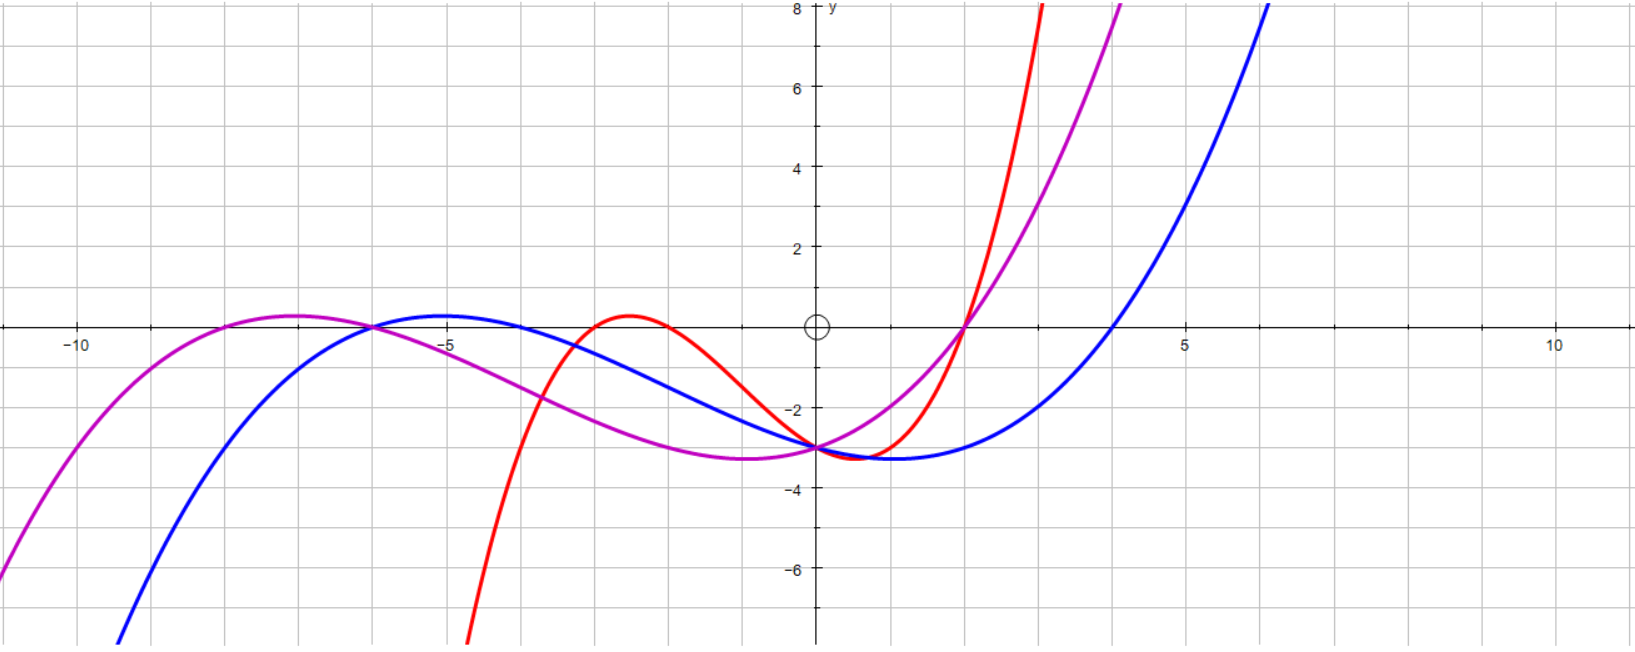
\includegraphics[width=\textwidth]{rootsofpolynomials}}
\end{figure}

\noindent
The roots of the \textcolor{red}{red} equation are $\alpha$, $\beta$ and $\gamma$; \newline
The roots of the \textcolor{blue}{blue} equation are $2\alpha$, $2\beta$ and $2\gamma$; \newline
The roots of the \textcolor{purple}{purple} equation are $2\alpha-1$, $2\beta-1$ and $2\gamma-1$; \newline \par

The \textcolor{purple}{purple} curve can be obtained by a sequence of transformations of the orginal, \textcolor{red}{red} curve.
\begin{itemize}
\item[]
\vspace{-0.25cm}
\begin{itemize}
\item[1)] Stretch in the $x$-direction by scale factor 2 (\textcolor{red}{$x$} $\rightarrow$ \textcolor{blue}{$\frac{1}{2}x$})
\vspace{-0.15cm}
\item[2)] Translation by vector \scriptsize $\begin{bmatrix}-1\\0\end{bmatrix}$ \normalsize (\textcolor{blue}{$x$} $\rightarrow$ \textcolor{purple}{$x+1$})
\end{itemize}
\end{itemize}

Therefore the original equation, 
\begin{equation*}
y=k(x-\alpha)(x-\beta)(x-\gamma)
\end{equation*}
can therefore be replaced by the substitution $x\rightarrow\frac{x+1}{2}$, to give
\begin{equation*}
y=k\left(\frac{x+1}{2}-\alpha\right)\left(\frac{x+1}{2}-\beta\right)\left(\frac{x+1}{2}-\gamma\right)
\end{equation*}
\vspace{-0.4cm}


\subsection{The modulus function}
\begin{itemize}
\item A Level M Year 2 \hspace{1cm} \phantom{ AS / } Pages 50 -- 59
\end{itemize} \par
The modulus function, $|x|$ gives the magnitude of a number. Graphs of modulus functions give a sharp turn\footnote{Unless the function never strictly crosses the $x$-axis, for example $f(x)=cos(x)+1$} at the $x$-axis, whereas a polynomial for instance may cut the axis. 
\vspace{-0.25cm}
\begin{align*}
|a|=|b| \;&\Longleftrightarrow\; a^{2}=b^{2} \;\Longleftrightarrow\; a=\pm b  \\
|x-a|<b \;&\Longleftrightarrow\; a-b<x<a+b  \\
x^{2} \leq y^{2} \;&\Longleftrightarrow\; |x|\leq |y| 
\end{align*}


\subsection{Loci}
\label{loci}
\begin{itemize}
\item A Level M AS / Year 1 \hspace{1cm} \phantom{ } Pages 87 -- 112
\end{itemize} \par
A locus (pl. loci) is a set of points which satisfy certain conditions, (e.g. a set of points a distance $a$ from the point $(x,y)$ is a circle of radius $a$ centred on $(x,y)$).
\vspace{0.5cm}


\subsection{Parametric curves}
\begin{itemize}
\item A Level M Year 2 \hspace{1cm} \phantom{ AS / } Pages 253 -- 258
\end{itemize} \par
Parametric curves are where the two axes are defined in terms of some other variable, for example
\vspace{-0.2cm}
\begin{align*}
x&=\cos(\theta) \\
y&=\sin(\theta)
\end{align*}
For the Cartesian form, these must be substituted in to give $y$ in terms of $x$, or vice versa.
\vspace{0.5cm}


\subsection{Polar coordinates}
\begin{itemize}
\item A Level M Year 2 \hspace{1cm} \phantom{ AS / } Pages 199 -- 209
\end{itemize}
Polar coordinates are defined in terms of the distance of the point from the origin (radius) and the anti-clockwise angle from the positive $x$-axis.
\begin{equation*}
\begin{Bmatrix} r, \mathrm{radius} \\ \theta, \mathrm{angular\; coordinate}\end{Bmatrix} \\
\end{equation*}
\begin{align*}
&\mathrm{Cartesian:} & &15=x^{2}+y^{2} \\
&\mathrm{Parametric:}&  &\begin{Bmatrix} x=2t-5 \\ y=3t \end{Bmatrix} \\
&\mathrm{Polar:}&  &r=a\left( 1+\frac{\theta}{\pi} \right)\text{ for } 0\leq\theta\leq2\pi\text{, }a>0
\end{align*}
\par
$r$ is constrained to $r\geq0$. The domain of $\theta$ is specified by context

\begin{figure}[H]
     \centering
         \scalebox{.8}{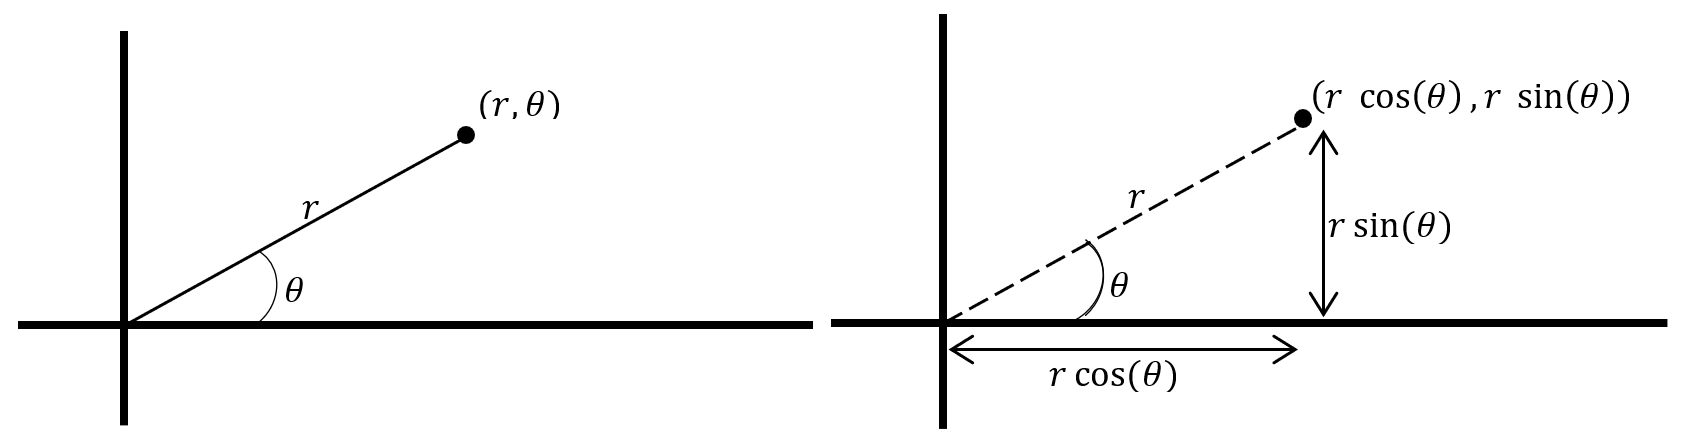
\includegraphics[width=\textwidth]{polarcoordinates}}
\end{figure}
To convert from polar $(r,\theta)$ to Cartesian form $(x,y)$,
\vspace{-0.2cm}
\begin{align*}
x&=r\cos(\theta) \\
y&=r\sin(\theta)
\end{align*}
To convert from Cartesian form $(x,y)$ to polar $(r,\theta)$
\begin{align*}
r&=\sqrt{x^{2} + y^{2}} \\
\theta&=\arctan\left(\frac{y}{x}\right)
\end{align*}
\vspace{0.5cm}


\clearpage
\section{Calculus I: Differentiation}
\vspace{0.5cm}

\subsection{Differentiation and derivatives -- Tangent and normal}
\begin{itemize}
\item A Level M AS / Year 1 \hspace{1cm} \phantom{ } Pages 251 -- 260 
\item A Level M AS / Year 1 \hspace{1cm} \phantom{ } Pages 271 -- 274
\end{itemize} \par
Differentiation of a function gives the instantaneous rate of change (tangent) to that function. 
From first principles, differentiation is defined as:
\begin{equation*}
f'(x)=\lim_{h \to 0}\left[ \frac{f(x+h)-f(x)}{h} \right]
\end{equation*}
This is explicitly the formula for the gradient of the chord $PQ$, where $P$ and $Q$ have coordinates $(x,f(x))$ and $(x+h,f(x+h))$ respectively, in the limit where $h$ tends to zero. \newline \par
Learning how to differentiate combinations of functions is also necessary. Intuitively, we can see that a simple addition (or subtraction) of functions $h(x)=f(x)\pm g(x)$ has a derivative $h'(x)=f'(x)\pm g'(x)$ by putting $h(x)$ into the definition above. Sections \ref{chainrule}, \ref{productrule}, and \ref{quotientrule} show how to differentiate pairs of functions combined in different ways. \newline \par
The derivative of a function at a point gives the gradient of the tangent at that point. The straight-line equation of the tangent to a point $(a,b)$ is given by
\begin{equation*}
y-b=m(x-a)
\end{equation*}
where $x$ and $y$ are general points in space, $a$ and $b$ are the coordinates of the specific point, and $m$ is the gradient of the tangent (value of the derivative). If we wish to find the equation of the straight-line normal to the point, that has a gradient equal to the negative reciprocal of the gradient of the tangent. \newline \par
Derivatives of a function $y=y(x)$ can be denoted by $\frac{\mathrm{d}y}{\mathrm{d}x}$ (Leibniz notation) or $y'(x)$ (Lagrange notation). Higher derivatives are expressed as $\frac{\mathrm{d}^{n}y}{\mathrm{d}x^{n}}$ (Leibniz) or $y^{(n)}(x)$ (Lagrange). For smaller values of $n$, Lagrange notation makes use of repeated primes ($'$), i.e. $y''(x)$, $y''(x)$, etc. but for higher $n$, this becomes unwieldy. \newline \par

Newton also introduced `dot-notation' for time derivatives. Conventionally, this is only used when dealing with functions of times, so for the function $x=x(t)$, $\dot{x}=\frac{\mathrm{d}x}{\mathrm{d}t}$, $\ddot{x}=\frac{\mathrm{d}^{2}x}{\mathrm{d}t^{2}}$, etc.
\vspace{0.5cm}


\subsection{Useful derivatives to know}
\label{usefulderivatives}
Here is a list of derivatives of simple functions. They can of course be manipulated in the usual way using the chain rule (section \ref{chainrule}), product rule (section \ref{productrule}), and quotient rule (section \ref{quotientrule}). 

\begin{figure}[H]
\centering
\begin{subfigure}[b]{0.49\textwidth}
\centering
\begin{tblr}{|[.75pt]|c|c||[.75pt]}
\hline[1.25pt]
\textbf{$f(x)$} & \textbf{$f'(x)$}  \\ \hline[0.75pt]
constant & 0 \\ \hline
$x^{n}$ & $nx^{n-1}$ \\ \hline
$e^{x}$ \small{\emph{or}} $\exp(x)$ &  $e^{x}$ \small{\emph{or}} $\exp(x)$ \\ \hline
$\ln(x)$ & $\frac{1}{x}$ \\ \hline
$\sin(x)$ & $\cos(x)$  \\ \hline
$\cos(x)$ & $-\sin(x)$  \\ \hline
$\tan(x)$ & $\sec^{2}(x)$  \\ \hline
$\sec(x)$ & $\sec(x)\tan(x)$  \\
\hline[.75pt]
\end{tblr}
\end{subfigure}
\hfill
\begin{subfigure}[b]{0.49\textwidth}
\centering
\begin{tblr}{|[.75pt]|c|c||[.75pt]}
\hline[1.25pt]
\large{\textbf{$f(x)$}} & \large{\textbf{$f'(x)$}}  \\ \hline[0.75pt]
$\cosec(x)$ & $-\cosec(x)\cotan(x)$  \\ \hline
$\cotan(x)$ & $-\cosec^{2}(x)$ \\ \hline
$\sinh(x)$ &  $\cosh(x)$ \\ \hline
$\cosh(x)$ & $\sinh(x)$ \\ \hline
$\tanh(x)$ & $\sech^{2}(x)$  \\ \hline
$\sech(x)$ & $-\sech(x)\tanh(x)$  \\ \hline
$\cosech(x)$ & $-\cosech(x)\coth(x)$  \\ \hline
$\coth(x)$ & $-\cosech^{2}(x)$  \\
\hline[.75pt]
\end{tblr}
\end{subfigure}
\end{figure}
\vspace{0.2cm}


\subsection{Finding stationary points and curve sketching}
\begin{itemize}
\item A Level M AS / Year 1 \hspace{1cm} \phantom{ } Pages 275 -- 279
\end{itemize} \par
Roots of an equation give $x$ intercepts; constant term (of a polynomial) gives the $y$ intercept. A single root is a basic cut, a double root is a local maximum or minimum, and a triple root is a stationary point of inflection. \newline \par 

Any stationary points are characterised by the first derivative being $0$.
\vspace{0.2cm}


\subsection{Classification of stationary points}
\begin{itemize}
\item A Level M Year 2 \hspace{1cm} \phantom{ AS / } Pages 247 -- 253
\item A Level M Year 2 \hspace{1cm} \phantom{ AS / } Pages 261 -- 267
\end{itemize} \par
The second derivative gives the gradient of the gradient of the function. Stationary points of a function $f(x)$ can be classified as follows:
\begin{equation*}
\mathrm{If\;} f'(a)=0 
\begin{cases}
f''(a)>0, & \mathrm{then\;} x=a\; \mathrm{is\; a\; minimum} \\
f''(a)<0, & \mathrm{then\;} x=a\; \mathrm{is\; a\; maximum} \\
f''(a)=0, & \text{then further investigation required}
\end{cases}
\end{equation*}
A point of inflection is a point where the second derivative changes sign $(+/-)$
\vspace{0.5cm}


\subsection{Curvature: convex, concave and point of inflection}
\begin{itemize}
\item A Level M Year 2 \hspace{1cm} \phantom{ AS / } Pages 247 -- 253
\end{itemize} \par
\begin{itemize}
\item[-] A function $f$ is said to be \underline{\textbf{convex}} over an interval $[a,b]$ if \\$f''(x)\geq0, \forall x \in[a,b]$
\item[-] A function $f$ is said to be \underline{\textbf{concave}} over an interval $[a,b]$ if \\$f''(x)\leq0, \forall x \in[a,b]$
\item[-] A \underline{\textbf{point of inflection}} on a curve $y=f(x)$ is a point where \\$f''(a)=0$ \emph{and} $f''(a)$ changes sign
\end{itemize}
\vspace{0.5cm}


\subsection{Optimisation}
\begin{itemize}
\item A Level M AS / Year 1 \hspace{1cm} \phantom{ } Pages 279 -- 287
\end{itemize} \par
Use first and second derivatives to find maximum or minimum values subject to sets of constraints
\vspace{0.5cm}


\subsection{The Chain Rule}
\label{chainrule}
\begin{itemize}
\item A Level M Year 2 \hspace{1cm} \phantom{ AS / } Pages 198 -- 202
\end{itemize} \par
The chain rule is used to differentiate \emph{composite functions} (functions of functions). It works as follows:
\begin{equation*}
\frac{\mathrm{d}}{\mathrm{d}x}\left[ f(g(x)) \right]=f'(g(x))\times g'(x)
\end{equation*}
A couple of examples:
\begin{align*}
\frac{\mathrm{d}}{\mathrm{d}x}\left[\sqrt{\text{something}}\right]&=\frac{1}{2\sqrt{\text{something}}}\times\frac{\mathrm{d}}{\mathrm{d}x}\left[\text{something}\right] \\
\frac{\mathrm{d}}{\mathrm{d}x}\left[\frac{1}{\text{something}}\right]&=-\frac{1}{\text{something}^{2}}\times\frac{\mathrm{d}}{\mathrm{d}x}\left[\text{something}\right] \\
\end{align*}
\begin{itemize}
\item[Note:] The chain rule must also be considered and applied when anti-differenti\-ating
\end{itemize}
\vspace{0.5cm}
\newpage

\subsection{The Product Rule}
\label{productrule}
\begin{itemize}
\item A Level M Year 2 \hspace{1cm} \phantom{ AS / } Pages 203 -- 205
\end{itemize} \par
The product rule is used to differentiate the \emph{product} of two functions. Here is a short derivation as to where it comes from.
\begin{figure}[H]
\centering
\begin{subfigure}[b]{0.49\textwidth}
\centering
\scalebox{.85}{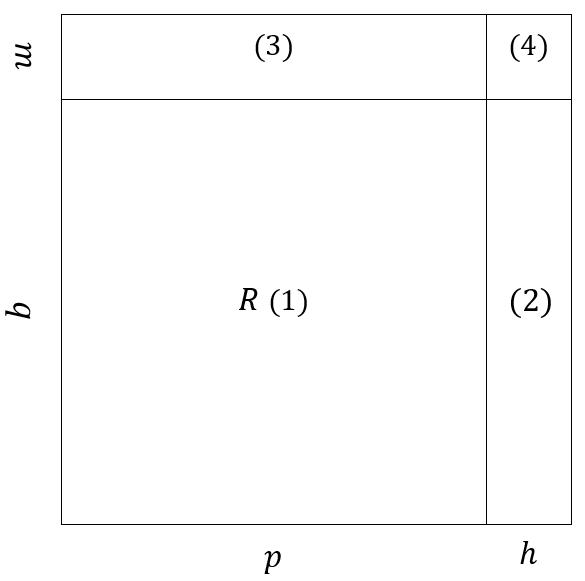
\includegraphics[width=\textwidth]{productrule1}}
\end{subfigure}
\hfill
\begin{subfigure}[b]{0.49\textwidth}
\small
First consider how the area $R$ changes when $p\rightarrow p+h$, and $q\rightarrow q+m$.
\begin{flalign*}
R&=p\cdot q, & R'=p'\cdot q' && \\
&&&&\\
R'&=(p+h)(q+m)& && \\
&=pq+hq+pm+hm & &&
\end{flalign*}
where $pq$, $hq$, $pm$, $hm$ are labelled $(1)$, $(2)$, $(3)$, and $(4)$ respectively. \\
\normalsize
\end{subfigure}
\end{figure}

\begin{figure}[H]
\centering
\begin{subfigure}[b]{0.49\textwidth}
\centering
\scalebox{.85}{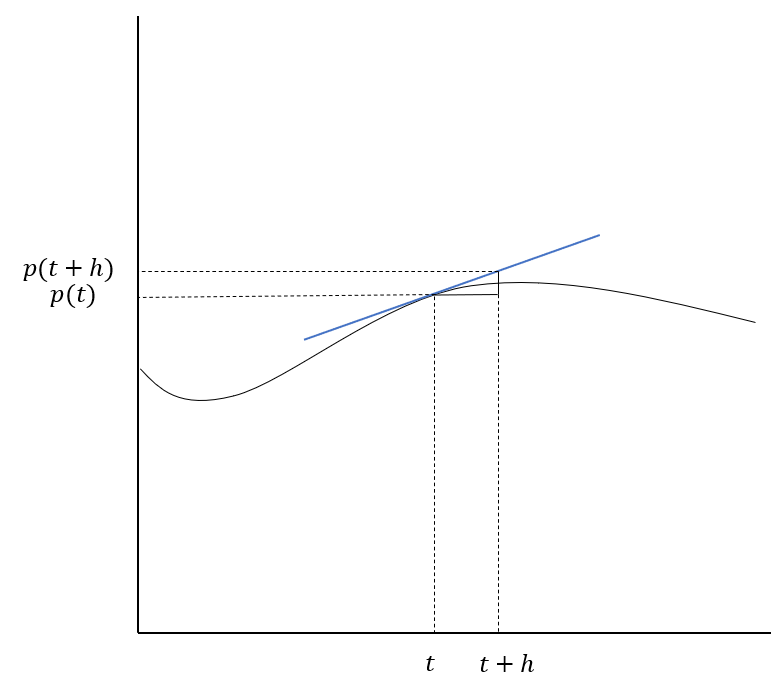
\includegraphics[width=\textwidth]{productrule3}}
\end{subfigure}
\hfill
\begin{subfigure}[b]{0.49\textwidth}
\small
Zooming in on the triangle created by the points $(t,p(t)), (t+h, p(t)), (t+h, p(t+h))$, we can approximate the distance from $p(t+h)$ to $p(t)$ by reversing our first principle form of a derivative, to give:
\normalsize
\begin{center}
\scalebox{.5}{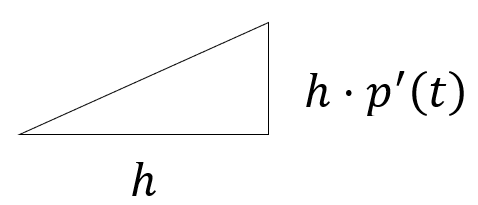
\includegraphics[width=\textwidth]{productrule2}}
\end{center}
So, we have: $p(t+h)\approx p(t)+h\times p'(t)$ \scriptsize{\emph{good if $h\rightarrow 0$}}
\normalsize
\end{subfigure}
\end{figure}
\vspace{-0.5cm}
Define $R(t)=p(t)\cdot q(t)$
\begin{flalign*}
R(t)&=p(t)\cdot q(t) && \\
R(t+h)&=p(t+h)\cdot q(t+h) && \\
R(t+h)&\approx (p(t)+h\times p'(t))\cdot (q(t)+h\times q'(t)) && \\
R(t+h)&\approx p(t)q(t)+h\left[ p'(t)q(t) + p(t)q'(t)  \right]+h^{2}\left[ p'(t)q'(t) \right] && \\
\end{flalign*}
This definition of $R(t+h)$ can then be used in the definition of the derivative from first principles;
\scriptsize
\begin{flalign*}
\frac{\mathrm{d}R}{\mathrm{d}t}&= \lim_{h \to 0} \left[ \frac{R(t+h)-R(t)}{h} \right] && \\
&= \lim_{h \to 0} \left[ \frac{\left( \cancel{p(t)q(t)}+h\left[ p'(t)q(t) + p(t)q'(t)  \right]+h^{2}\left[ p'(t)q'(t) \right] \right)-\cancel{p(t)q(t)}}{h} \right] && \\
&= \lim_{h \to 0} \left[ \frac{\cancel{h}\left[ p'(t)q(t) + p(t)q'(t)  \right]+h^{\cancel{2}}\left[ p'(t)q'(t) \right]}{\cancel{h}} \right] && \\
&=p'(t)q(t)+p(t)q'(t)+\cancel{\lim_{h\to0}\left[ h\left[p'(t)q'(t)\right] \right]} \\
\frac{\mathrm{d}R}{\mathrm{d}t}&=  p'(t)q(t) + p(t)q'(t) &&
\end{flalign*}
\normalsize
So we recover the \emph{Product Rule}
\begin{equation*}
\frac{\mathrm{d}}{\mathrm{d}x}\left[ f(x)g(x) \right] = f'(x)g(x)+f(x)g'(x)
\end{equation*}
%\vspace{0.5cm}


\subsection{The Quotient Rule}
\label{quotientrule}
\begin{itemize}
\item A Level M Year 2 \hspace{1cm} \phantom{ AS / } Pages 206 -- 209
\end{itemize} \par
The quotient rule is used to differentiate the \emph{quotient} of two functions. While a quotient is still a product, the product rule reduces to a simpler form in the case of a quotient, and so it is given a separate name. The derivation relies on the results of the chain rule and product rule (sections \ref{chainrule} and \ref{productrule} respectively).

\small
\begin{flalign*}
\frac{f(x)}{g(x)} &= f(x)g(x)^{-1} \hspace{2.75cm} \frac{\mathrm{d}}{\mathrm{d}x}\left[ g(x)^{-1} \right]=-[g(x)]^{2}\times g'(x) && \\
\frac{\mathrm{d}}{\mathrm{d}x} \left[ \frac{f(x)}{(g(x)} \right] &= \frac{\mathrm{d}}{\mathrm{d}x}\left[ f(x)\left[ g(x) \right]^{-1} \right] && \\
&=f'(x)\left[ g(x) \right]^{-1} + \left[ - \left[ g(x) \right]^{-2} \times g'(x) \right]\times f(x) && \\
&=\frac{f'(x)}{\left[ g(x) \right]} - \frac{f(x)g'(x)}{\left[ g(x) \right]^{2}} && \\
&=\frac{f'(x)g(x)}{\left[ g(x) \right]^{2}} - \frac{f(x)g'(x)}{\left[ g(x) \right]^{2}} && \\
&=\frac{f'(x)g(x)-f(x)g'(x)}{\left[ g(x) \right]^{2}} && \\
\end{flalign*}
\normalsize

Therefore, the \emph{Quotient Rule} is:
\begin{equation*}
=\frac{f'(x)g(x)-f(x)g'(x)}{\left[ g(x) \right]^{2}}
\end{equation*}
\vspace{0.1cm}

\newpage
\subsection{Implicit differentiation}
\label{implicitdifferentiation}
\begin{itemize}
\item A Level M Year 2 \hspace{1cm} \phantom{ AS / } Pages 209 -- 214
\end{itemize} \par
Implicit differentiation works in the same way as the chain rule, with the correction factor of a $y$ term being $\frac{\mathrm{d}y}{\mathrm{d}x}$. This is best illustrated by an example:
\begin{flalign*}
\frac{\mathrm{d}}{\mathrm{d}x}\left[ \left(x^{2}+4\right)^{3}\right]&=3\left( x^{2}+4\right)^{2}\times 2x && \\
&=6x\left(x^{2}+4\right)^{2} && \\
\frac{\mathrm{d}y}{\mathrm{d}x}\left[ \left( f(x)\right)^{3}\right]&=3\left( f(x) \right)^{2}\times\frac{\mathrm{d}}{\mathrm{d}x}\left[ f(x) \right] &&\\
\frac{\mathrm{d}y}{\mathrm{d}x}\left[ y^{3}\right]&=3y^{2}\times\frac{\mathrm{d}y}{\mathrm{d}x}&&
\end{flalign*} \par
\vspace{0.5cm}

\subsection{Differentiating inverse functions}
\begin{itemize}
\item A Level M Year 2 \hspace{1cm} \phantom{ AS / } Pages 214 -- 216
\end{itemize} \par
$f(x)=y$, so $x=f^{-1}(y)$ Therefore $f'(x)=\frac{\mathrm{d}y}{\mathrm{d}x}$, and by extension, the derivative of the inverse function is equal to $\frac{\mathrm{d}x}{\mathrm{d}y}=\frac{1}{\left(\frac{\mathrm{d}y}{\mathrm{d}x}\right)}$. \newline \par

This method can be used to find the derivative of inverse functions, and extends to functions such as $\arcsin, \arcosh, \ln, \text{\emph{etc.}}$. For example, take the function $y=\ln(x)$:
\begin{flalign*}
x&=e^{y} \hspace{2.75cm} y=\ln(x) && \\
\frac{\mathrm{d}y}{\mathrm{d}x}&=e^{y} && \\
\frac{\mathrm{d}y}{\mathrm{d}x}&= \frac{1}{\left(\frac{\mathrm{d}x}{\mathrm{d}y}\right)} =e^{-y} =e^{-\ln(x)}=x^{-1} =\frac{1}{x} &&
\end{flalign*}
\vspace{0.2cm}


\subsection{Parametric differentiation}
\label{parametricdifferentiation}
\begin{itemize}
\item A Level M Year 2 \hspace{1cm} \phantom{ AS / } Pages 258 -- 263
\end{itemize} \par
Parametric equations are defined in terms of an external variable, for example:
\begin{gather*}
x=f(t)\\y=g(t)
\end{gather*}
Therefore, $\frac{\mathrm{d}x}{\mathrm{d}t}=f'(t)$ and $\frac{\mathrm{d}y}{\mathrm{d}t}=g'(t)$, so:
\begin{equation*}
\frac{\mathrm{d}y}{\mathrm{d}x}=\frac{\left( \frac{\mathrm{d}y}{\mathrm{d}t} \right)}{\left( \frac{\mathrm{d}x}{\mathrm{d}t} \right)}=\frac{g'(t)}{f'(t)}
\end{equation*}
\begin{itemize}
\item[Note:] See section \ref{relatedratesofchange} for more on why we can `cancel' the $dt$ terms as with fractions
\end{itemize}
\vspace{0.5cm}


\subsection{Sketching curves}
\begin{itemize}
\item A Level M AS / Year 1 \hspace{1cm} \phantom{ } Pages 55 -- 68
\end{itemize} \par
When sketching curves, think about:
\begin{itemize}
\item[-] Intersections
\vspace{-0.25cm}
\item[-] Intercepts on axes
\vspace{-0.25cm}
\item[-] Which curves are above / below other curves (and where crossovers occur)
\vspace{-0.25cm}
\item[-] Derivatives $\rightarrow$ stationary points
\vspace{-0.25cm}
\item[-] Behaviour for large positive and negative $x$
\vspace{-0.25cm}
\item[-] Asymptotes (vertical, horizontal, oblique)
\end{itemize}
\vspace{0.5cm}


\subsection{Rational functions; polynomial curve sketching}
\begin{itemize}
\item A Level M AS / Year 1 \hspace{1cm} \phantom{ } Pages 55 -- 68
\end{itemize} \par
A rational function is defined as any function which can be expressed as a rational fraction of polynomials. \newline \par

When sketching, take out a factor of the denominator from the numerator to give the horizontal / oblique asymptote. \newline \par

For example:
\begin{flalign*}
y&=\frac{-x^{3}+5x}{x^{2}-4} && \\
&=\frac{-x\left( x^{2}-4\right)+x}{x^{2}-4} && \\
&=-x+\frac{x}{(x+2)(x-2)} \hspace{1cm} (*)
\end{flalign*}
This implies the oblique asymptote is $y=-x$, as $\lim_{x\rightarrow\pm\infty}\left[ \frac{x}{(x+2)(x-2)} \right]=0$, so for large positive and negative $x$, $y$ tends to $-x$. It is trivial to see $x=2$ and $x=-2$ are vertical asymptotes, as they are roots of the expression in the denominator, and dividing by zero is undefined. \newline \par

Lastly, we need to consider whether the curve approaches the horizontal / oblique asymptote from above or below, and whether the vertical asymptotes have the function going to positive or negative infinity. To do this, consider the parity of the numerator and denominator as $x$ approaches the vertical asymptote limits from above and below. So, in the case of $y=\frac{-x^{3}+5x}{x^{2}-4}$:

\scriptsize
\begin{center}
\begin{tblr}{|[.75pt]|c||c|c||[.75pt]}
\hline[1.25pt]
$x$ & $-2^{-}$ & $-2^{+}$ \\ \hline[.75pt]
Numerator & $-(-2^{-})^{3}+5(-2^{-})=-2^{-}<0$ & $-(-2^{+})^{3}+5(-2^{+})=-2^{+}<0$ \\ \hline
Denominator & $(-2^{-})^{2}-4=0^{+}>0$ & $(-2^{+})^{2}-4=0^{-}<0$ \\ \hline
Asymptote & $y=\frac{-2^{-}}{0^{+}}=-\infty$ & $y=\frac{-2^{+}}{0^{-}}=+\infty$ \\ 
\hline[.75pt]
\end{tblr}
\end{center}
\normalsize

\scriptsize
\begin{center}
\begin{tblr}{|[.75pt]|c||c|c||[.75pt]}
\hline[1.25pt]
$x$ &  $2^{-}$ & $2^{+}$ \\ \hline[.75pt]
Numerator & $-(2^{-})^{3}+5(2^{-})=2^{-}>0$ & $-(2^{+})^{3}+5(2^{+})=2^{+}>0$ \\ \hline
Denominator & $(2^{-})^{2}-4=0^{-}<0$ & $(2^{+})^{2}-4=0^{+}>0$ \\ \hline
Asymptote & $y=\frac{2^{-}}{0^{-}}=-\infty$ & $y=\frac{2^{+}}{0^{+}}=+\infty$ \\ 
\hline[.75pt]
\end{tblr}
\end{center}
\normalsize

We can then see from $(*)$, considering `remainder' of the asymptote, the denominator tends to $0^{+}$ as $x$ tends to $\pm\infty$. So, the parity of the `remainder' is determined by the parity of the numerator in this case, which is simply $x$. So, for $x\rightarrow+\infty$, the remainder is positive, and for $x\rightarrow-\infty$, the remainder is negative. Thus the curve approaches the asymptote from above for $x\rightarrow+\infty$ and from below for $x\rightarrow-\infty$. \newline \par

To see what all of this looks like, the figure below has the curve in red, with the asymptotes marked on in dashed lines:

\begin{figure}[H]
\centering
\begin{subfigure}[b]{0.89\textwidth}
\centering
\scalebox{0.85}{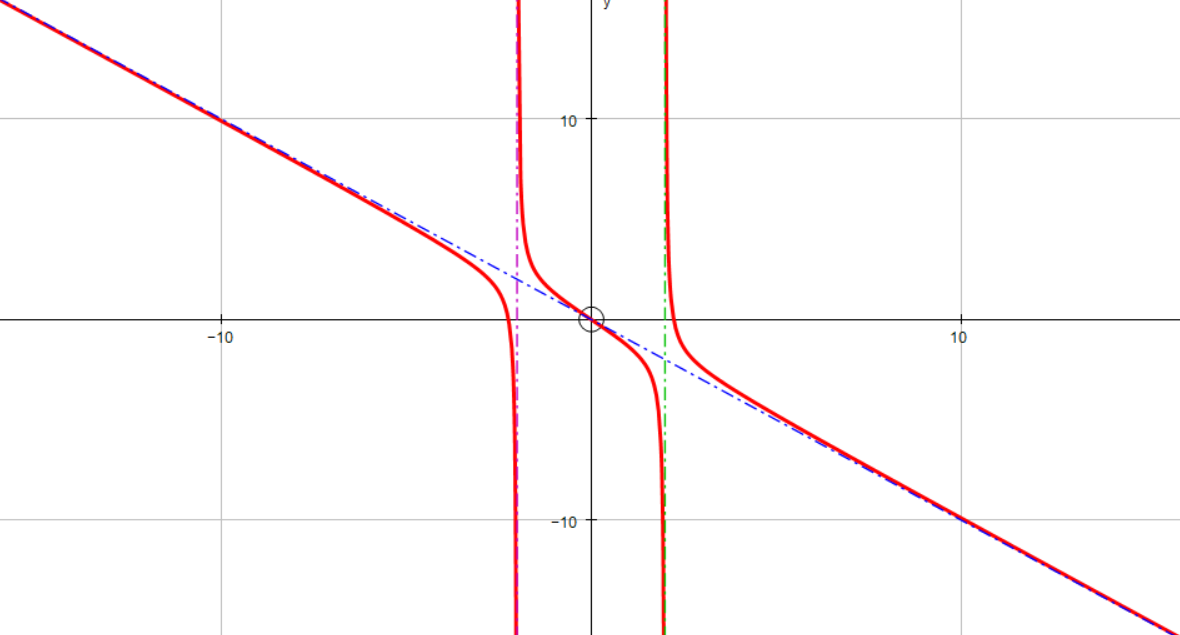
\includegraphics[width=\textwidth]{curvesketching}}
\end{subfigure}
\end{figure}

\vspace{0.5cm}



\clearpage
\section{Calculus II: Integration}
\vspace{0.5cm}


\subsection{Anti-differentiation}
\begin{itemize}
\item A Level M AS / Year 1 \hspace{1cm} \phantom{ } Pages 291 -- 300
\end{itemize} \par
Anti-differentiation is the act of taking a function and finding a function which gives your starting function as a derivative. For example: 
\begin{flalign*}
\frac{\mathrm{d}y}{\mathrm{d}x}=x^{n} \;\Longleftrightarrow\; y=\frac{1}{n+1}x^{n+1}+c \hspace{1.75cm} \text{where }c\text{ is any intercept} &&
\end{flalign*}
We use the integral sign, $\int$ to denote an anti-derivative.
\begin{flalign*}
&\int f(x)+g(x)\, \mathrm{d}x=\int f(x)\, \mathrm{d}x+\int g(x)\, \mathrm{d}x && \\
&\int k\cdot f(x)\, \mathrm{d}x=k\cdot\int f(x)\,\mathrm{d}x &&\\
&\int 3x^{4}-x^{-2}\,\mathrm{d}x=\frac{3}{5}x^{5}+x^{-1}+c && \\
&\int x^{n}\,\mathrm{d}x =\frac{1}{n+1}x^{n+1}+c \hspace{2.75cm} (n\neq 1) && \\
\end{flalign*}
While this is trivial for simple functions, such as polynomials (as above), there are various other methods that can be used, which are detailed in subsequent sections. The list of useful derivatives in section \ref{usefulderivatives} will continue to be useful for anti-differentiation / integration.
\vspace{0.5cm}


\subsection{Integration}
\begin{itemize}
\item A Level M AS / Year 1 \hspace{1cm} \phantom{ } Pages 291 -- 310
\item A Level M Year 2 \hspace{1cm} \phantom{ AS / } Pages 269 -- 277
\end{itemize} \par
Integration is anti-differentiation of specific areas. When evaluated with limits, it calculates the \emph{signed area}. If the curve goes below the $x$-axis, the area is evaluated as negative. When integrating the area  between two curves, find the area beneath each curve, and subtract from one another, or do the single integral of $(\int\left[\mathrm{Top\,-\,Bottom}\right]\,\mathrm{d}x)$

\scriptsize
\begin{flalign*}
\int_{0.5}^{2}-x^{2}+2x+3\,\mathrm{d}x &= \left[ -\frac{x^{3}}{3}+x^{2}+3x\, (+c) \right]_{0.5}^{2} && \\
&=\left[ -\frac{(2)^{3}}{3}+(2)^{2}+3(2)\, (+c) \right]-\left[ -\frac{(0.5)^{3}}{3}+(0.5)^{2}+3(0.5)\, (+c) \right] && \\
&=\frac{45}{8}+\left[ c-c \right] \hspace{1.5cm} \text{The $c$ terms cancel, so not necessary to include}
\end{flalign*}
\normalsize
\vspace{0.3cm}


\subsection{Integration by inspection}
\begin{itemize}
\item A Level M Year 2 \hspace{1cm} \phantom{ AS / } Pages 219 -- 223
\end{itemize}
If you are lucky, you may be able to spot the impact of a chain rule on an integrand, and so can give a good guess as to the result of the integral. For example
\begin{equation*}
\int \frac{x}{x^{2}+1}\,\mathrm{d}x=\frac{1}{2}\ln\left( x^{2}+1 \right)+c
\end{equation*}
Since by use of the chain rule, the derivative of the argument of $\ln$ is a factor of the numerator of the fraction. A further example is
\begin{equation*}
\int \tan(x)\,\mathrm{d}x=\int \frac{\sin(x)}{\cos(x)}\,\mathrm{d}x=-\ln(\cos(x))
\end{equation*}
As the derivative of $\cos(x)$ is $\sin(x)$ which appears in the numerator.
\vspace{0.5cm}


\subsection{Integration by parts}
\begin{itemize}
\item A Level M Year 2 \hspace{1cm} \phantom{ AS / } Pages 230 -- 234
\end{itemize} \par
This method is useful when evaluating the integral of product of two functions. Assuming the function $f(x)$ can be re-written as $u(x)\times\frac{\mathrm{d}v}{\mathrm{d}x}$. Then by using the results of the product rule, it converts the integral into a form that \emph{may} be easier to solve. 
\small
\begin{flalign*}
\frac{\mathrm{d}}{\mathrm{d}x}\left[ u(x)\cdot v(x) \right]&=u(x)\times\frac{\mathrm{d}v}{\mathrm{d}x}+\frac{\mathrm{d}u}{\mathrm{d}x}\times v(x)  \hspace{1cm} \text{Take anti-derivative of both sides}&&\\
u(x)\cdot v(x)&=\int\,\left[ u(x)\times\frac{\mathrm{d}v}{\mathrm{d}x}+\frac{\mathrm{d}u}{\mathrm{d}x}\times v(x) \right]\mathrm{d}x&&\\
&=\int\,\left[ u(x)\times\frac{\mathrm{d}v}{\mathrm{d}x} \right] \mathrm{d}x+\int \left[ \frac{\mathrm{d}u}{\mathrm{d}x}\times v(x) \right]\mathrm{d}x
\end{flalign*}\\ \normalsize
Therefore, integration by parts can be expressed as:
\begin{equation*}
\int u(x)\times \frac{\mathrm{d}v}{\mathrm{d}x}\,\mathrm{d}x=u(x)\cdot v(x)-\int v(x)\times \frac{\mathrm{d}u}{\mathrm{d}x} \, \mathrm{d}x
\end{equation*} \\
Or, when evaluated with limits;
\begin{equation*}
\int_{a}^{b} u(x)\times \frac{\mathrm{d}v}{\mathrm{d}x}\,\mathrm{d}x=\left[ u(x)\cdot v(x) \right] _{a}^{b}-\int_{a}^{b} v(x)\times \frac{\mathrm{d}u}{\mathrm{d}x} \, \mathrm{d}x
\end{equation*}

How do you decide which part of the integrand to be $u$, and which to be $\frac{\mathrm{d}v}{\mathrm{d}x}$? The acronym `\emph{LIATE}' can help pick a `$u$' function. If any component of the integrand is one of the following, then this should be chosen to be the `$u$' function, with priority given to logarithms, then inverse trigonometrics, etc.
\begin{center}
\begin{tblr}{|[.75pt]|c|l|l||[.75pt]}
\hline[.75pt]
\emph{L} & Logarithm & i.e. $\ln{(x)}$, $\log{(x)}$ \\ \hline
\emph{I} & Inverse trigonometric & i.e. $\arcsin(x)$, $\arccos(x)$ \\ \hline
\emph{A} & Algebraic & i.e. $3x^{2}+1$, polynomials \\ \hline
\emph{T} & Trigonometric & i.e. $\tan(x)$, $\sin(x)$ \\ \hline
\emph{E} & Exponential & i.e. $e^{x}$, $\sinh(x)$ \\ \hline[.75pt]
\end{tblr}
\end{center}
\vspace{0.5cm}

\subsection{Integration by substitution}
\begin{itemize}
\item A Level M Year 2 \hspace{1cm} \phantom{ AS / } Pages 223 -- 230
\end{itemize} \par
This involves making a substitution for $x$ which makes the integral easier to solve. For example, the substitution $u=3x-2$ makes the following integral considerably easier to solve:
\begin{equation*}
\int_{2}^{3}x\sqrt{3x-2}\,\mathrm{d}x=\int_{4}^{7}\frac{(u+2)}{3}\sqrt{u}\times\frac{\mathrm{d}x}{\mathrm{d}u}\,\mathrm{d}u
\end{equation*}
\emph{Note: The limits must be changed too, to be consistent with the substitution} \newline \par
Since the scale of the axis is different, the correction factor is $\frac{\mathrm{d}x}{\mathrm{d}u}$ This can be thought of as the two $\mathrm{d}u$ terms cancelling, leaving the integration with respect to $x$. \newline \par
When performing an \emph{indefinite integral}, the result comes out in terms of $u$, so $x$ must be substituted back into the result. A definite integral does not need this, since the limits are also changed according to the substitution. Section \ref{usefulintegrals} contains some useful integral substitutions. 
\vspace{0.5cm}


\subsection{Standard integrals}
\label{usefulintegrals}
\begin{itemize}
\item A Level FM Year 2 \hspace{1cm} \phantom{AS /} Pages 157 -- 163
\end{itemize} \par
Here are some integrals which substitutions make considerably simpler. These are \underline{all} in the formula booklet, so while it is good to recognise them, there is no need to memorise the substitutions required in each case.

\begin{center}
\begin{tblr}{|[.75pt]|c|c||[.75pt]}
\hline[1.25pt]
$f(x)$ & $\int f(x)\,\mathrm{d}x$ \\ \hline[.75pt]
$\frac{1}{\sqrt{a^{2}-x^{2}}}$ & $\sin^{-1}\left(\frac{x}{a}  \right)$ for $\left( |x|<a \right)$ \\ \hline
$\frac{1}{a^{2}+x^{2}}$ & $\frac{1}{a}\tan^{-1}\left(\frac{x}{a}  \right)$  \\ \hline
$\frac{1}{\sqrt{a^{2}-x^{2}}}$ & $\sinh^{-1}\left(\frac{x}{a}  \right)$ or $\ln\left( x+\sqrt{x^{2}+a^{2}} \right)$  \\ \hline
$\frac{1}{\sqrt{x^{2}-a^{2}}}$ & $\cosh^{-1}\left(\frac{x}{a}  \right)$ or $\ln\left( x+\sqrt{x^{2}-a^{2}} \right)$ for $x>a$  \\ \hline[.75pt]
\end{tblr}
\end{center}
\vspace{0.5cm}


\subsection{Integration by partial fractions}
\begin{itemize}
\item A Level M Year 2 \hspace{1cm} \phantom{ AS / } Pages 239 -- 243
\item A Level FM Year 2 \hspace{1cm} \phantom{AS /} Pages 163 -- 166
\end{itemize} \par
Rational functions, for example $\frac{7x+4}{(x+2)(2x-1)}$ can be re-written in partial fractions (see sections \ref{partialfractions1} and \ref{partialfractions2} for more on how to do this). In this case, it decomposes into $\frac{2}{x+2}+\frac{3}{2x-1}$. This \emph{may} make the integration of a rational function easier.
\vspace{0.5cm}


\subsection{Improper integrals}
\begin{itemize}
\item A Level FM Year 2 \hspace{1cm} \phantom{AS /} Pages 179 -- 183
\end{itemize} \par
Some functions are undefined at certain points (i.e $\frac{1}{1-x}$ is undefined at $x=1$) and so the integral is undefined too; other integrals are over an infinite range, and so these integrals are called \emph{improper}.

\begin{flalign*}
&\int_{0}^{\infty}e^{-3x}\,\mathrm{d}x &&\text{is improper because the range of integration is infinite} && \\
&\int_{0}^{3}\frac{1}{\sqrt{3-x}}\,\mathrm{d}x &&\text{is improper because the integrand is undefined at $x=3$} && \\
&\int_{1}^{\infty} \frac{1}{x}\,\mathrm{d}x &&\text{is improper because the range of integration is infinite} &&
\end{flalign*}

We can deal with these types of integrals by setting the undefined integral limit to a variable (let us say $b$ in this case), and then take the limit as $b$ tends to the indeterminate limit. This is best illustrated by an example:
\newpage
\begin{flalign*}
\int_{0}^{\infty}e^{-3x}\,\mathrm{d}x &= \lim_{b \to \infty}\left[ \int_{0}^{b}e^{-3x}\,\mathrm{d}x \right] && \\
&=\lim_{b\to\infty}\left[ \left[ -\frac{1}{3}e^{-3x}\right]_{0}^{b}\right] && \\
&=\lim_{b\to\infty}\left[ -\frac{1}{3}e^{-3b}--\frac{1}{3}e^{0} \right] && \\
&=\lim_{b\to\infty}\left[-\frac{1}{2}e^{-3b}+\frac{1}{3}\right] &&
\end{flalign*}
And as $b\rightarrow\infty$, $-\frac{1}{3}e^{-3b}\rightarrow0$, so $\int_{0}^{\infty}e^{-3x}\,\mathrm{d}x=\frac{1}{3}$\\
Therefore the integral  $\int_{0}^{\infty}e^{-3x}\,\mathrm{d}x$ \emph{does} exist, or converges, and has value $\frac{1}{3}$ \newline \par

\begin{flalign*}
\int_{0}^{3}\frac{1}{\sqrt{3-x}}\,\mathrm{d}x &= \lim_{b \to 3}\left[ \int_{0}^{3}\frac{1}{\sqrt{3-x}}\,\mathrm{d}x \right] && \\
&=\lim_{b\to3}\left[ \left[ -2\sqrt{3-x}\right]_{0}^{b}\right] && \\
&=\lim_{b\to3}\left[ \left[ -2\sqrt{3-b} - -2\sqrt{3-0}\right]_{0}^{b}\right] && \\
&=2\sqrt{3} &&
\end{flalign*}
Therefore the integral  $\int_{0}^{3}\frac{1}{\sqrt{3-x}}\,\mathrm{d}x$ \emph{does} exist, or converges, and has value $2\sqrt{3}$ \newline \par

\begin{flalign*}
\int_{0}^{\infty}\frac{1}{x}\,\mathrm{d}x &= \lim_{b\to\infty}\left[ \left[ \ln(x)\right]_{0}^{b}\right] && \\
&=\lim_{b\to\infty}\left[ \ln(b)-\ln(0) \right] && \\
&=\lim_{b\to\infty}\left[-\frac{1}{2}e^{-3b}+\frac{1}{3}\right] &&
\end{flalign*}
However as $b\rightarrow\infty$, $\ln(b)\rightarrow\infty$, so $\int_{0}^{\infty}\frac{1}{x}\,\mathrm{d}x$ is not defined.\\
\begin{itemize}
\item[Note:] If the integrand is undefined between the limits, we must evaluate the integral between each of the limits and the point at which it is undefined.
\end{itemize}
\vspace{0.5cm}

\subsection{Polar integration}
\begin{itemize}
\item A Level FM Year 2 \hspace{1cm} \phantom{AS /} Pages 210 -- 216
\end{itemize} \par
\begin{figure}[H]
\centering
\begin{subfigure}[b]{0.49\textwidth}
Polar integration measures the area `swept out' by the curve, as opposed to the area directly beneath it. \newline \par

We can use a triangle approximation, whereby:
\vspace{-0.2cm}
\begin{equation*}
\text{Area of a triangle}=\frac{1}{2}ab\sin(C)
\end{equation*}
\end{subfigure}
\hfill
\begin{subfigure}[b]{0.49\textwidth}
\centering
\scalebox{.85}{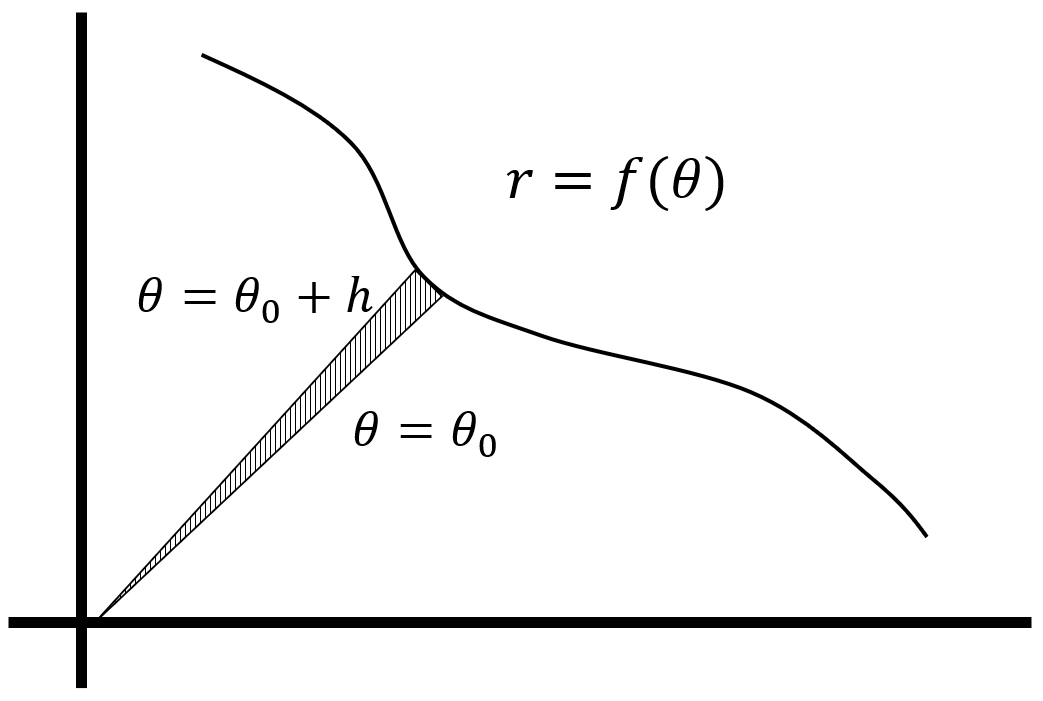
\includegraphics[width=\textwidth]{polarintegration}}
\end{subfigure}
\end{figure}
So, the area swept out by the triangle is:
\begin{flalign*}
&=\lim_{h\to0}\left[ \frac{1}{2}\times f(\theta_{0})\times f(\theta_{0}+h)\times\sin(h) \right] && \\
&\textcolor{white}{=\;\;}f(\theta_{0}+h)\rightarrow f(\theta_{0})\text{ and }\sin(h)\rightarrow h\text{, so} &&\\
&=\frac{1}{2}\times f(\theta_{0})^{2}\times h &&
\end{flalign*}
The area swept out by the curve is then the sum of the triangles.
\begin{flalign*}
Area&=\sum triangles &&=\sum \frac{1}{2}f(\theta_{0})^{2}h &&=\int\frac{1}{2}f(\theta_{0})^{2}\,\mathrm{d}\theta &&\\
&&\\
Area&=\int\frac{1}{2}r^{2}\,\mathrm{d}\theta &&
\end{flalign*}
\vspace{0.5cm}


\subsection{The Trapezium Rule}
\begin{itemize}
\item A Level M Year 2 \hspace{1cm} \phantom{ AS / } Pages 331 -- 341
\end{itemize} \par
In order to estimate the area of a curve without integrating, the area can be approximated by summing a series of trapezia between the limits. The number of divisions between the limits determines the accuracy of the approximation. 
\begin{figure}[H]
\centering
\begin{subfigure}[b]{0.49\textwidth}
\centering
\scalebox{1.2}{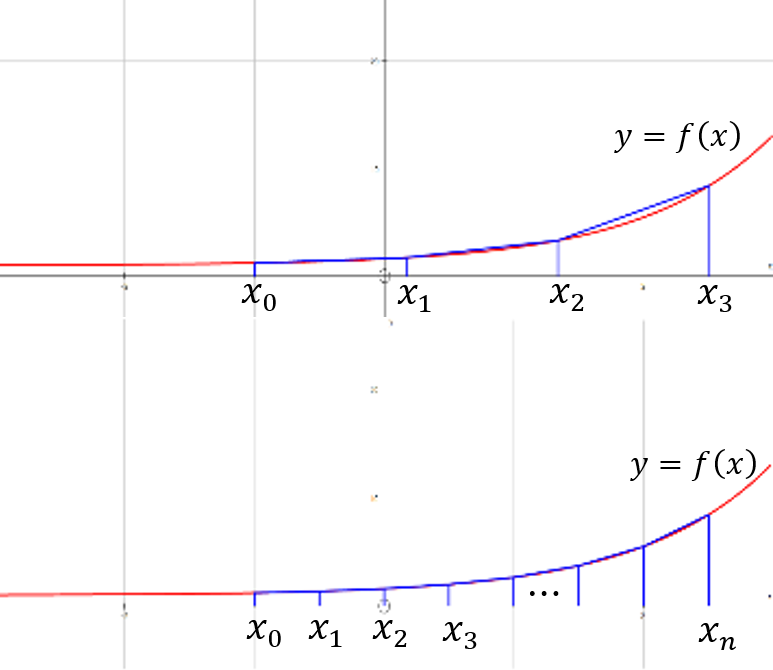
\includegraphics[width=\textwidth]{trapeziumrule}}
\end{subfigure}
\end{figure}
\noindent So, this approximate sum can be written as:
\begin{flalign*}
\int_{x_{0}}^{x^{n}}f(x)\,\mathrm{d}x&=\sum_{k=0}^{n-1}\left[ \left( y_{k}+y_{k+1}\right)\times\frac{h}{2} \right] && \\
\int_{x_{0}}^{x^{n}}f(x)\,\mathrm{d}x&=\frac{h}{2}\left[ y_{0}+2\left( y_{1}+y_{2}+\cdots+y_{n-2}+y_{n-1}\right)+y_{n}\right] &&
\end{flalign*}
\vspace{0.5cm}


\subsection{Parametric integration}
\begin{itemize}
\item A Level M Year 2 \hspace{1cm} \phantom{ AS / } Pages 263 -- 265
\end{itemize} \par
Used to integrate a curve given by a set of parametric equations, where the limits may be given in terms of the additional parameter, $t$, as opposed to in terms of $x$.
\begin{figure}[H]
\centering
\begin{subfigure}[b]{0.39\textwidth}
\begin{flalign*}
&\begin{Bmatrix}x=f(t) \\ y=g(t)\end{Bmatrix} \Rightarrow \frac{\mathrm{d}y}{\mathrm{d}x}=\frac{\left(\frac{\mathrm{d}y}{\mathrm{d}t}\right)}{\left(\frac{\mathrm{d}x}{\mathrm{d}t}\right)} &&\\
&&\\
&\int_{a}^{b}y\,\mathrm{d}x=\int_{t=t_{0}}^{t=t_{1}}y\frac{\mathrm{d}x}{\mathrm{d}t}\,\mathrm{d}t &&\\
&&
\end{flalign*}
\end{subfigure}
\hfill
\begin{subfigure}[b]{0.59\textwidth}
\centering
\scalebox{1}{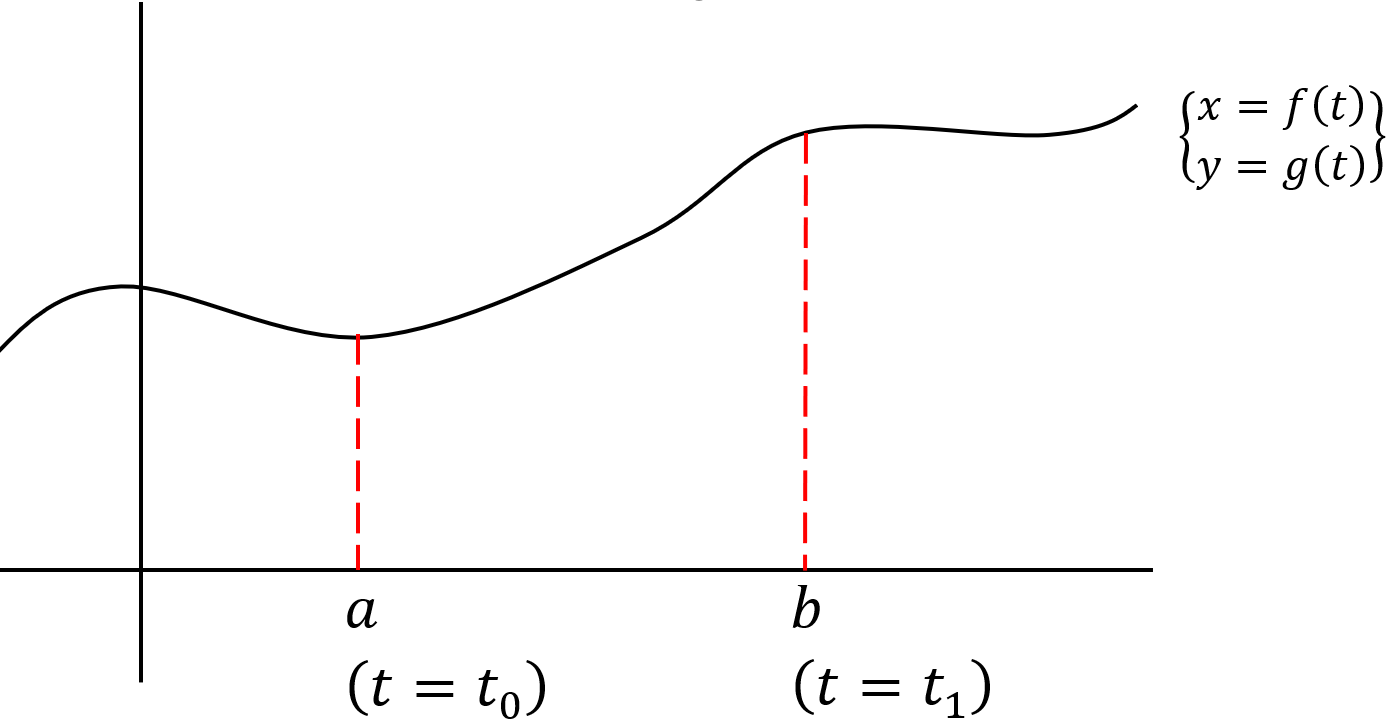
\includegraphics[width=\textwidth]{parametricintegration}}
\end{subfigure}
\end{figure}
\vspace{0.5cm}


\subsection{Volumes of revolution}
\begin{itemize}
\item A Level FM Year 2 \hspace{1cm} \phantom{AS /} Pages 183 -- 190
\end{itemize} \par
A volume of revolution is the volume obtained by rotating a curve around an axis, and then taking the volume enclosed by the surface created.
\begin{figure}[H]
\centering
\begin{subfigure}[b]{0.59\textwidth}
When we calculate a definite integral, one way of thinking about it is summing up the areas of infinitely small rectangles. Therefore when we calculate a volume of revolution, we can consider it to be a sum of the volumes of infinitely thin cylinders. \newline \par
\end{subfigure}
\hfill
\begin{subfigure}[b]{0.39\textwidth}
\centering
\scalebox{1}{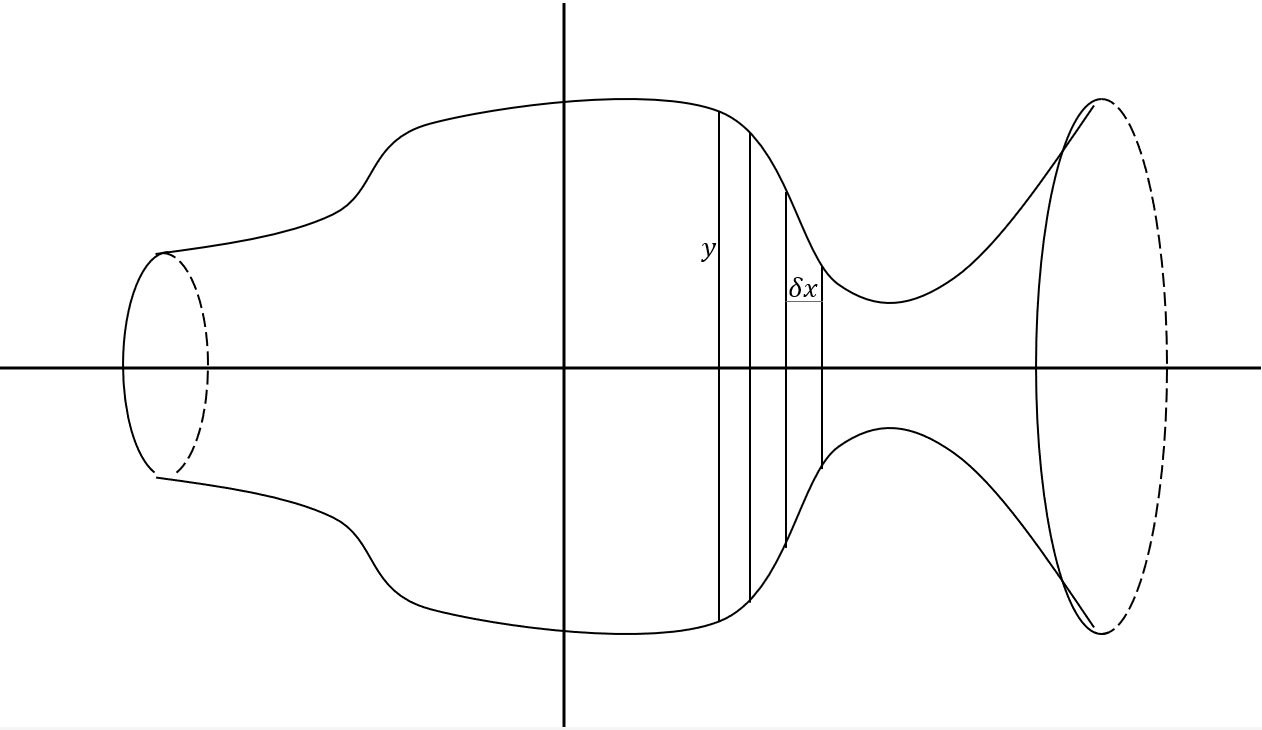
\includegraphics[width=\textwidth]{volumesofrevolution1}}
\end{subfigure}
\end{figure}
\noindent The volume of each cylinder is $V_{\text{cylinder}}=\pi r^{2}h$, where:\\
The radius, $r$, is the height of the curve at theat point, ($r=y$) \\
The height, $h$, is the width of each cylinder $\delta x$ \\
\begin{flalign*}
\text{So }V_{\text{cylinder}}&=\pi y^{2} \delta x & &&\\
\text{So }V_{\text{Total}}&=\sum V_{\text{cylinders}} && \\
&=\sum \pi y^{2} \delta x  & \text{As $\delta x \rightarrow 0$, becomes an infinitessimal sum}&& \\
&=\int\pi y^{2}\,\mathrm{d}x &&
\end{flalign*}
If doing this with parametric equations,
\begin{equation*}
V_{\text{Total}}=\int\pi\cdot y(t)^{2}\cdot\frac{\mathrm{d}x}{\mathrm{d}t}\,\mathrm{d}t
\end{equation*}

If rotating about the $y$-axis, then all the $x$ terms are swapped with $y$ terms.

\vspace{0.5cm}


\clearpage
\section{Trigonometry}
\vspace{0.5cm}


\subsection{Trigonometric values of sin, cos, and tan}
\begin{itemize}
\item A Level M AS / Year 1 \hspace{1cm} \phantom{ } Pages 177 -- 179
\end{itemize} \par
These should all be familiar from GCSE, and while this table is identical to that in section \ref{radianmeasure}, the contents of it remain just as important.
\begin{center}
\begin{tblr}{|[.75pt]|c|c||c|c|c||[.75pt]}
\hline[1.25pt]
$\theta$ in $^{\circ}$ & $\theta$ in radians & $\sin(\theta)$ & $\cos(\theta)$ & $\tan(\theta)$ \\ \hline[.75pt]
$0$ & $0$ & $0$ & $1$ & $0$ \\ \hline
$30$ & $\frac{\pi}{6}$ & $\frac{1}{2}$ & $\frac{\sqrt{3}}{2}$ & $\frac{1}{\sqrt{3}}$ \\ \hline
$45$ & $\frac{\pi}{4}$ & $\frac{1}{\sqrt{2}}$ & $\frac{1}{\sqrt{2}}$ & $1$ \\ \hline
$60$ & $\frac{\pi}{3}$ & $\frac{\sqrt{3}}{2}$ & $\frac{1}{2}$ & $\sqrt{3}$ \\ \hline
$90$ & $\frac{\pi}{2}$ & $1$ & $0$ & $\mathrm{undefined}$ \\ \hline[1pt]
\end{tblr}
\end{center}

\vspace{0.5cm}


\subsection{Sine and cosine rules; area formulae}
\begin{itemize}
\item A Level M AS / Year 1 \hspace{1cm} \phantom{ } Pages 204 -- 217
\end{itemize} \par
These all should be familiar from GCSE;

\begin{table}[H]
\renewcommand{\arraystretch}{1.25}
\begin{tabular}{ll}
Area: & $\frac{ab\sin(C)}{2}=\frac{bc\sin(A)}{2}=\frac{ca\sin(B)}{2}$ \\
Sine rule: & $\frac{a}{\sin(A)}=\frac{b}{\sin(B)}=\frac{c}{\sin(C)}$ \\
Cosine rule: & $a^{2} = b^{2} + c^{2} - 2bc\cos(A)$ \\
\end{tabular}
\end{table}
\vspace{0.5cm}


\subsection{Sine, cosine and the unit circle}
The unit circle is defined by
\begin{equation*}
(x,y)=(\cos(\theta),\sin(\theta))
\end{equation*}
So:
\begin{equation*}
x^{2}+y^{2}=\cos^{2}(\theta)+\sin^{2}(\theta)=1
\end{equation*}
$\tan(\theta)$ gives the gradient of the normal to points on the circle. This can be shown using parametric differentiation (section \ref{parametricdifferentiation})

\vspace{0.5cm}


\subsection{Trigonometric equations, and the Pythagorean identity}
\begin{itemize}
\item A Level M AS / Year 1 \hspace{1cm} \phantom{ } Pages 179 -- 188
\item A Level M Year 2 \hspace{1cm} \phantom{ AS / } Pages 178 -- 182
\end{itemize} \par
We recognise from GCSE the standard trigonometric functions $\sin$, $\cos$ and $\tan$, and that $\tan$ of an angle is defined as the ratio between $\sin$ and $\cos$ $\left(\tan(\theta)\equiv\frac{\sin(\theta)}{\cos(\theta)}\right)$. We can also define the reciprocal trigonometric functions as follows:
\small
\begin{align*}
\cosec(\theta)&=\frac{1}{\sin(\theta)} & \sec(\theta)&=\frac{1}{\cos(\theta)} & \cot(\theta)=\frac{1}{\tan(\theta)}=\frac{\cos(\theta)}{\sin(\theta)}
\end{align*}
\normalsize
We can therefore manipulate the Pythagorean identity,
\begin{equation*}
\sin^{2}(\theta)+\cos^{2}(\theta)\equiv1
\end{equation*}
To give two more identities by dividing through by $\sin^{2}$ or $\cos^{2}$:
\begin{align*}
1+\cot^{2}(\theta)&=\cosec^{2}(\theta) & \tan^{2}(\theta)+1&=\sec^{2}(\theta)
\end{align*}
\normalsize

\vspace{0.5cm}


\subsection{The small-angle approximations}
\begin{itemize}
\item A Level M Year 2 \hspace{1cm} \phantom{ AS / } Pages 155 -- 163
\end{itemize} \par
The small angle approximations for $\sin$, $\cos$, and $\tan$ are as follows:
\begin{figure}[H]
\centering
\begin{subfigure}[b]{0.49\textwidth}
\begin{flalign*}
\sin(\theta)&\approx\theta &&\\
\cos(\theta)&\approx1-\frac{1}{2}\theta^{2} && \\
\tan(\theta)&\approx\theta
\end{flalign*}
\end{subfigure}
\hfill
\begin{subfigure}[b]{0.49\textwidth}
\centering
\scalebox{.85}{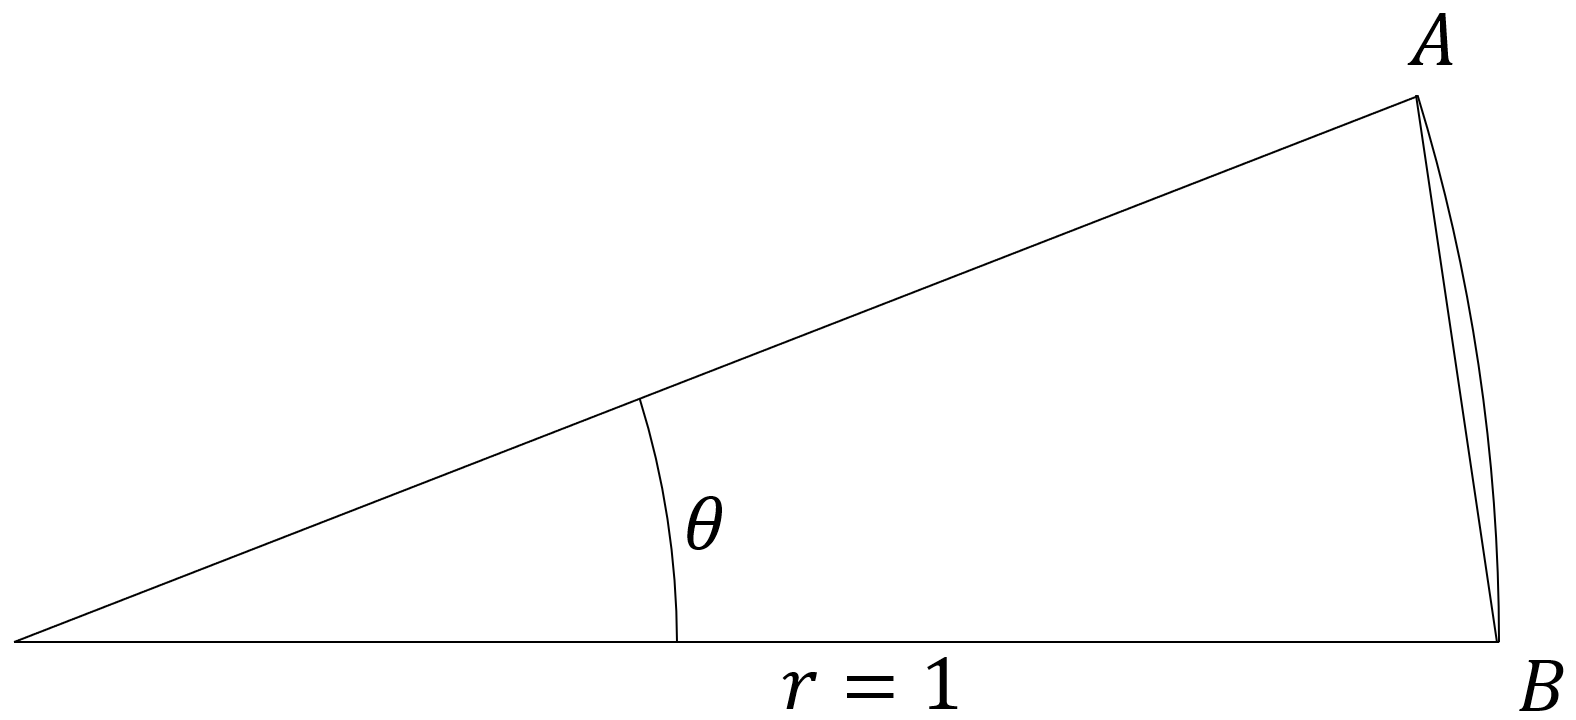
\includegraphics[width=\textwidth]{smallangleapproximation1}}
\end{subfigure}
\end{figure}
\scriptsize
\begin{itemize}
\item[Note:]These are the first terms of the Maclaurin series (see section \ref{standardmaclaurin}) for each of these
\end{itemize}
\normalsize
The arc $AB$ has length $\theta$ (in radians of course), and the chord $AB$ has length $\sin(\theta)$. When $\theta$ is samll:
\begin{flalign*}
AB_{\text{arc}}&\approx AB_{\text{chord}} && \\
\theta&\approx\sin(\theta) &&
\end{flalign*}

We can use a double angle identity (section \ref{doubleangleformulae}) to express $\cos(\theta)$ in terms of $\sin\left(\frac{1}{2}\theta\right)$ terms alone, and thus gain an approximation for $\cos$:
\newpage
\vspace{-.3cm}
\begin{flalign*}
\cos(\theta)&=1-2\sin^{2}\left( \frac{1}{2}\theta \right) && \\
\cos(\theta)&\approx1-2\cdot\left( \frac{1}{2}\theta \right)^{2} && \\
\cos(\theta)&=1-\frac{1}{2}\theta^{2}
\end{flalign*}

Constructing an approximation using this method for $\tan$ requires a little more work, but can still be done relatively easily. First, we assume a quadratic approximation for $\tan(\theta)$, and then substitute in our approximations for $\sin$ and $\cos$ into $\sin(\theta)=\tan(\theta)\cdot\cos(\theta)$:
\begin{flalign*}
\tan(\theta)&\approx p+q\theta+r\theta^{2} && \\
&&&\\
\sin(\theta)&\approx p\cdot\cos(\theta)+q\theta\cdot\cos(\theta)+r\theta^{2}\cdot\cos(\theta) && \\
\theta&\approx p-\frac{p\theta^{2}}{2}+q\theta-\frac{q\theta^{3}}{2}+r\theta^{2}-\frac{r\theta^{4}}{2} && \\
0&\approx p+\theta(q-1)+\theta^{2}(r-\frac{p}{2})+\theta^{3}(-\frac{q}{2})+\theta^{4}(-\frac{r}{2}) &&
\end{flalign*}
Now since we only need terms up to the quadratic;
\begin{flalign*}
p&=0 &&\\
q-1&=0 \hspace{1cm}\Rightarrow \hspace{1cm}q=1 &&\\
r-\frac{p}{2}&=0 \hspace{1cm}\Rightarrow \hspace{1cm}r=0 &&
\end{flalign*}

Therefore;
\begin{flalign*}
\tan(\theta)&\approx0+1\cdot\theta+0\cdot\theta^{2} && \\
\tan(\theta)&\approx\theta &&
\end{flalign*}
\vspace{0.5cm}


\subsection{Double angle formulae}
\label{doubleangleformulae}
\begin{itemize}
\item A Level M Year 2 \hspace{1cm} \phantom{ AS / } Pages 168 -- 173
\end{itemize} \par
A geometric derivation for the double angle formulae for $\sin$, $\cos$, and $\tan$ is provided here. A matrix method can also be used, which extends the validity of these formulae to all $\theta$.
\begin{figure}[H]
\centering
\scalebox{.95}{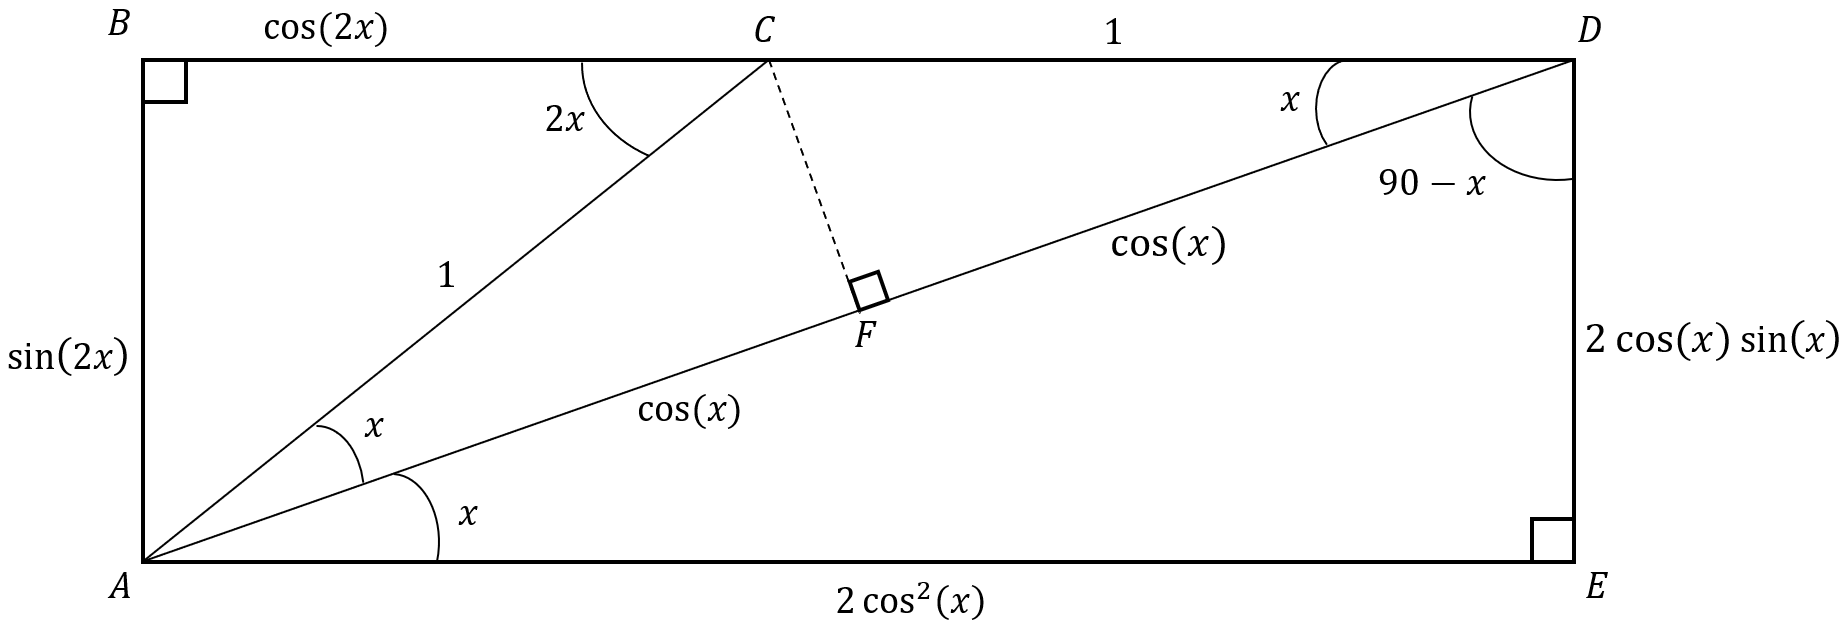
\includegraphics[width=\textwidth]{doubleangleformulae}}
\end{figure}
Define the rectangle $ABDE$ such that $D\hat{A}E=x$, and position $C$ along $BD$ such that $AC=CD=1$.
\begin{flalign*}
C\hat{D}A&=x & & \text{(alternate angles)} && \\
C\hat{A}D&=x & & \text{(isosceles triangle)} && \\
C\hat{A}E&=2x & & && \\
A\hat{C}B&=2x & & \text{(alternate angles)} && \\
AB&=\sin(2x) & & \text{(trigonometric relation)} && \\
BC&=\cos(2x) & & \text{(trigonometric relation)} && \\
AF&=FD=\cos(x) & & \text{($CF$ is a perpendicular bisector)} && \\
AD&=2\cos(x) & & AF+FD=AD && \\
AE&=2\cos(x)\times\cos(x)=2\cos^{2}(x) & & \text{(trigonometric relation)} && \\
DE&=2\cos(x)\sin(x) & & \text{trigonometric relation)} && \\
& & & && \\
AB&=DE & \Rightarrow &\sin(2x)=2\cos(x)\sin(x) && \\
BD&=AE & \Rightarrow &\cos(2x)=2\cos^{2}(x)-1 &&
\end{flalign*}

\begin{flalign*}
\frac{\sin(2x)}{\cos(2x)}&=\frac{2\cos(x)\sin(x)}{\cos^{2}(x)-\sin^{2}(x)} && \\
\tan(2x)&=\frac{2\cos(x)\sin(x)}{\cos^{2}(x)-\sin^{2}(x)} &=\frac{\frac{2\cos(x)\sin(x)}{cos^{2}(x)}}{\frac{\cos^{2}(x)-\sin^{2}(x)}{\cos^{2}(x)}} &=\frac{2\frac{\sin(x)}{\cos(x)}}{\frac{\cos^{2}(x)}{\cos^{2}(x)}-\frac{\sin^{2}(x)}{\cos^{2}(x)}} && \\
& && \\
\tan(2x)&=\frac{2\tan(x)}{1-\tan^{2}(x)}
\end{flalign*}

So, the \emph{double angle formulae} are as follows:
\begin{align*}
\cos(2\theta)&\equiv 
\begin{cases}
\cos^{2}(\theta)-\sin^{2}(\theta) \\
2\cos^{2}(\theta)-1 \\
1-2\sin^{2}(\theta)
\end{cases} \\
\sin(2\theta)&\equiv 2\sin(\theta)\cos(\theta) \\
\tan(2\theta)&\equiv \frac{2\tan(\theta)}{1-\tan^{2}(\theta)}
\end{align*}

These can be used as substitutions when integrating functions involving terms of $\cos^{2}$ and $\sin^{2}$
\begin{itemize}
\item[Note:] The double angle formulae can be obtained from the \emph{compound angle formulae} (see section \ref{compoundangleformulae}) by setting $A=B$, which are given in the formula booklet.
\end{itemize}
\vspace{0.2cm}


\subsection{Compound angle formulae}
\label{compoundangleformulae}
\begin{itemize}
\item A Level M Year 2 \hspace{1cm} \phantom{ AS / } Pages 165 -- 167
\end{itemize} \par
A geometric derivation for the compound angle formulae for $\sin$, $\cos$, and $\tan$ is provided here. A matrix method can also be used, which extends the validity of these formulae to all $\theta$, which is also briefly demonstrated. While the matrix method is a quicker way of deriving them should you need to, they are also given in the formula booklet.

\subsubsection*{Geometric method}
\begin{figure}[H]
\centering
\scalebox{.95}{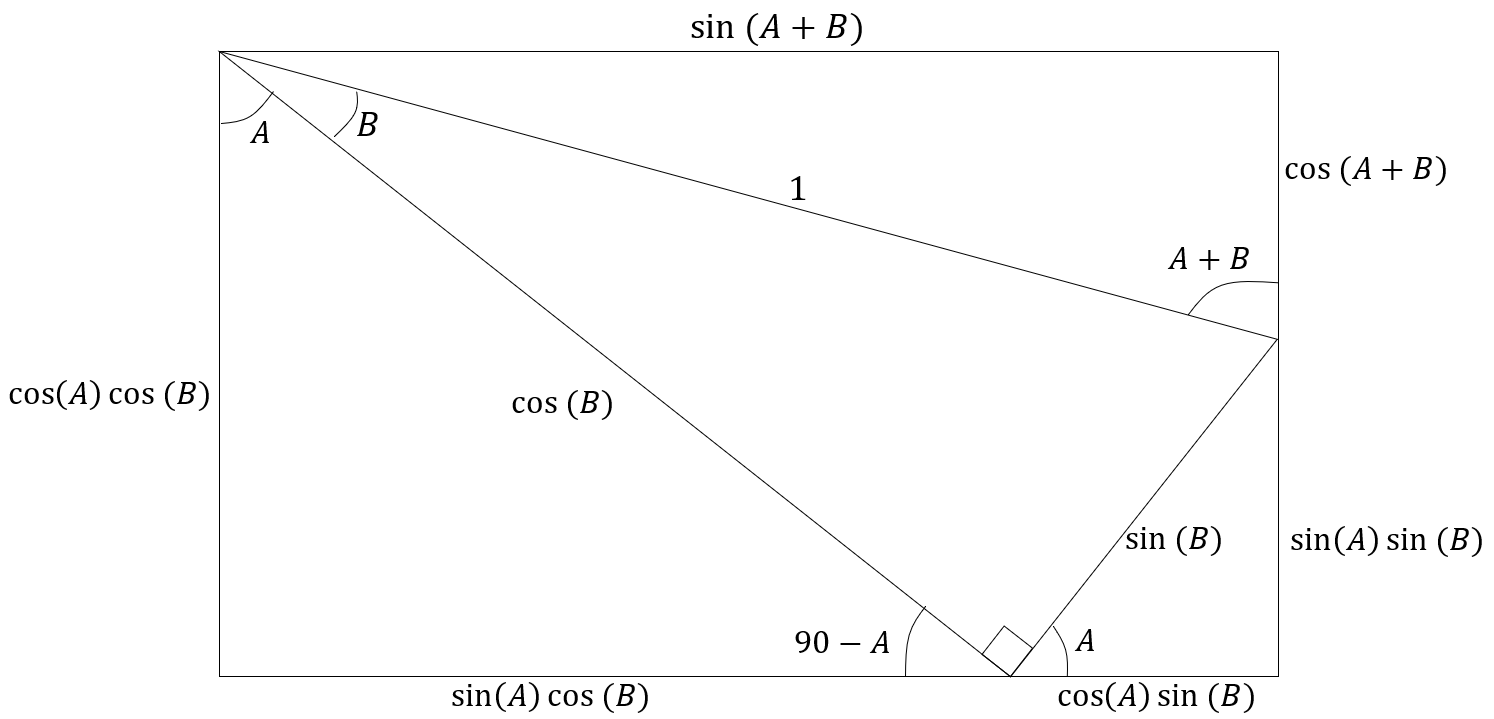
\includegraphics[width=\textwidth]{compoundangleformulae1}}
\end{figure}
The figure has all the side lengths marked on using simple trigonometric relations, and by rescaling such that a particular side has length 1 with two of the angles of size $A$ and $B$ (marked), the compound angle formulae follow quite straightforwardly:
\begin{align*}
\sin(A+B)&=\sin(A)\cos(B)+\cos(A)\sin(B) \\
\cos(A+B)&=\cos(A)\cos(B)-\sin(A)\sin(B) \\
\tan(A+B)&=\frac{\tan(a)+\tan(B)}{1-\tan(A)\tan(B)}
\end{align*}

By replacing $B$ with $-B$, we get the angle difference formulae. This can be deduced using the even / odd nature of $\sin$ and $\cos$.
\begin{align*}
\sin(A-B)&=\sin(A)\cos(B)-\cos(A)\sin(B) \\
\cos(A-B)&=\cos(A)\cos(B)+\sin(A)\sin(B) \\
\tan(A-B)&=\frac{\tan(a)-\tan(B)}{1+\tan(A)\tan(B)}
\end{align*}\par
\begin{itemize}
\item[Note:] This is only valid for positive angles less than $90^{\circ}$ / $\frac{\pi}{2}$ rad.
\end{itemize}

\subsubsection*{Matrix method}
The matrix $M=\begin{pmatrix} \cos(\theta) & -\sin(\theta) \\ \sin(\theta) & \cos(\theta) \end{pmatrix}$ represents a rotation of angle $\theta^{\circ}$ anticlockwise.
\begin{multline*}
\begin{pmatrix} \cos(\theta) & -\sin(\theta) \\ \sin(\theta) & \cos(\theta) \end{pmatrix} \begin{pmatrix} \cos(\phi) & -\sin(\phi) \\ \sin(\phi) & \cos(\phi) \end{pmatrix} \\ =\begin{pmatrix} \cos(\theta)\cos(\phi)-\sin(\theta)\sin(\phi) & -\left( \sin(\theta)\cos(\phi)-\cos(\theta)\sin(\phi) \right) \\ \sin(\theta)\cos(\phi)-\cos(\theta)\sin(\phi) & \cos(\theta)\cos(\phi)-\sin(\theta)\sin(\phi) \end{pmatrix}
\end{multline*}

Combined, this shows a rotation of an angle $\theta^{\circ}$ followed by a rotation of an angle $\phi^{\circ}$. Alternatively, this could be achieved by a single matrix representing a rotation of $(\theta+\phi)^{\circ}$ with elements:
\begin{equation*}
\begin{pmatrix} \cos(\theta+\phi) & -\sin(\theta+\phi) \\ \sin(\theta+\phi) & \cos(\theta+\phi) \end{pmatrix}
\end{equation*}
The compound angle formulae can then be trivially read off by matching the matrix elements. This also extends the validity to any angles $\theta$ and $\phi$.
\vspace{0.5cm}


\subsection{Harmonic Form -- superposition of waves of the same frequency}
\begin{itemize}
\item A Level M Year 2 \hspace{1cm} \phantom{ AS / } Pages 173 -- 178
\end{itemize} \par
This is a method that superimposes two (or more) waves which are of the \underline{same frequency}. It employs the compound angle formulae (see section \ref{compoundangleformulae}) to combine the two waves into a singular wave with some amplitude and phase shift. See below for a couple of worked examples.
\small
\begin{flalign*}
& && \\
\frac{\sqrt{3}}{2}\sin(x)-\frac{1}{2}\cos(x)&=\sin(x)\cos\left(\frac{\pi}{6}\right)-\cos(x)\sin\left(\frac{\pi}{6}\right) && \\
&=\sin\left(x-\frac{\pi}{6}\right) && \\
& && \\
\sin(x)+\cos(x)&=\sqrt{2}\left( \frac{1}{\sqrt{2}}\sin(x) + \frac{1}{\sqrt{2}}\cos(x) \right) && \\
&=\sqrt{2}\left(\cos\left(\frac{\pi}{4}\right)\sin(x)+\sin\left(\frac{\pi}{4}\right)\cos(x)\right) && \\
&=\sqrt{2}\cos\left(x-\frac{\pi}{4}\right) &&
\end{flalign*}
\normalsize

These are `nice' examples, where the phase shift is an easy factor to compute. More often than not, the examples will not be as trivial. A slightly more general way of answering these questions follows. Some questions may ask specifically for the combined wave to be a $\sin$ or $\cos$ wave with a phase shift. This can be done very simply by choosing the right form of $\sin(A\pm B)$ or $\cos(A\pm B)$. The choice of $+$ or $-$ is completely arbitrary, but a considered choice can make life much simpler. \newline \par

Take for example the expression $3\cos(x)-4\sin(x)$. Suppose we want to write this as a single cosine wave. This can be done as follows:
\begin{flalign*}
3\cos(x)-4\sin(x) &= R\cos(x+\alpha) && \\
&=R\cos(\alpha)\cos(x)-R\sin(\alpha)\sin(x) &&
\end{flalign*}
Collecting terms of $\cos(x)$ and $\sin(x)$ alike;
\begin{flalign*}
3\cos(x)&=R\cos(\alpha)\cos(x) & 3=R\cos(\alpha) && \\
4\sin(x)&=R\sin(\alpha)\sin(x) & 4=R\sin(\alpha) &&
\end{flalign*}
\begin{flalign*}
\frac{R\sin(\alpha)}{R\cos(\alpha)}&=\frac{4}{3} & R^{2}\sin^{2}(\alpha)&=16 && \\
\tan(\alpha)&=\frac{4}{3} & R^{2}\cos^{2}(\alpha)&=9 && \\
\alpha&=\arctan\left(\frac{4}{3}\right)+n\pi & R^{2}\left( \sin^{2}(\alpha)+\cos^{2}(\alpha) \right)&=25 && \\
& & R^{2}&= 25 \hspace{0.25cm} \Rightarrow \hspace{0.25cm} R=5 &&
\end{flalign*}
\footnotesize{Take principle value of $\alpha$ provided correct choice of $+$/$-$ earlier, so that $0\leq\alpha\leq\frac{\pi}{2}$} \newline \par
\normalsize

Thus;
\begin{equation*}
3\cos(x)-4\sin(x)=5\cos\left( x+\arctan\left(\frac{4}{3}\right) \right)
\end{equation*}\par

Suppose we wanted this in the form of $R\cos(x\textcolor{red}{-}\alpha)$. The expansion has the difference of a `$+$' instead of a `$-$' between the two terms involving $\cos(x)$ and $\sin(x)$. \par
\begin{flalign*}
3\cos(x)-4\sin(x) &= R\cos(x\textcolor{red}{-}\alpha) && \\
&=R\cos(\alpha)\cos(x)\textcolor{red}{+}R\sin(\alpha)\sin(x) &&
\end{flalign*}
Again, collecting terms of $\cos(x)$ and $\sin(x)$ alike;
\begin{flalign*}
3\cos(x)&=R\cos(\alpha)\cos(x) & 3=R\cos(\alpha) && \\
\textcolor{red}{-}4\sin(x)&=R\sin(\alpha)\sin(x) & \textcolor{red}{-}4=R\sin(\alpha) &&
\end{flalign*}
\begin{flalign*}
\frac{R\sin(\alpha)}{R\cos(\alpha)}&=\frac{\textcolor{red}{-}4}{3} & R^{2}\sin^{2}(\alpha)&=16 && \\
\tan(\alpha)&=\frac{\textcolor{red}{-}4}{3} & R^{2}\cos^{2}(\alpha)&=9 && \\
\alpha&=\arctan\left(\frac{\textcolor{red}{-}4}{3}\right)+n\pi & R^{2}\left( \sin^{2}(\alpha)+\cos^{2}(\alpha) \right)&=25 && \\
& & R^{2}&= 25 \hspace{0.25cm} \Rightarrow \hspace{0.25cm} R=5 &&
\end{flalign*}

Thus;
\begin{align*}
3\cos(x)-4\sin(x)&=5\cos\left( x\textcolor{red}{-}\arctan\left(\frac{\textcolor{red}{-}4}{3}\right) \right) \\
&=5\cos\left( x\textcolor{red}{+}\arctan\left(\frac{4}{3}\right) \right)
\end{align*}
as expected. \newline \par
Of course, we could also have chosen to write this in terms of a sine wave, again with free choice of whether it is $+\alpha$ or $-\alpha$ in the argument.
\vspace{0.5cm}


\subsection{The inverse trigonometric functions}
\begin{itemize}
\item A Level M Year 2 \hspace{1cm} \phantom{ AS / } Pages 134 -- 139
\end{itemize} \par
As stated in the section on inverse functions (section \ref{inversefunctions}) the graph of the inverse function can be obtained by a reflection in the line $y=x$. However, if the domains and codomains are left unrestricted, then the inverse function will be multi-valued for all of $\sin$, $\cos$, and $\tan$, which is not allowed for a function if it is to be properly defined (see section \ref{formalisingfunctions}). The domains and codomains for the three trigonometric functions are listed below, with the inverse functions swapping the restricted domain and codomain.


\begin{center}
\small
\begin{tblr}{|[.75pt]|l||c|c|c||[.75pt]}
\hline[1.25pt]
 & $\sin$ & $\cos$ & $\tan$ \\ \hline[.75pt]
Unrestricted & $\mathbb{R}\rightarrow[-1,1]$ & $\mathbb{R}\rightarrow[-1,1]$ & $\mathbb{R}\setminus\left\{ \pm\frac{\pi}{2},\pm\frac{3\pi}{2},\dots \right\} \rightarrow \mathbb{R}$ \\ \hline
Restricted & $\left[ -\frac{\pi}{2},\frac{\pi}{2} \right]\rightarrow[-1,1]$ & $\left[ 0,\pi \right]\rightarrow[-1,1]$ & $\left( -\frac{\pi}{2},\frac{\pi}{2} \right) \rightarrow \mathbb{R}$ \\ \hline
Inverse &  $\left[ -1,1 \right]\rightarrow[-\frac{\pi}{2},\frac{\pi}{2}]$ & $\left[ -1,1 \right]\rightarrow[0,\pi]$ & $\mathbb{R} \rightarrow \left( -\frac{\pi}{2},\frac{\pi}{2} \right)$ \\ \hline[1pt]
\end{tblr}
\normalsize
\end{center}

\vspace{0.5cm}


\subsection{Derivatives of sine and cosine}
\begin{itemize}
\item A Level M Year 2 \hspace{1cm} \phantom{ AS / } Pages 185 -- 195
\end{itemize} \par
The derivatives of trigonometric functions are closely linked and are set out below. A proof follows, though there are other ways of proving this.
\begin{center}
\begin{tblr}{|[.75pt]|c|c||[.75pt]}
\hline[1.25pt]
$f(x)$ & $\frac{\mathrm{d}}{\mathrm{d}x}\left[ f(x) \right]$ \\ \hline[.75pt]
$\sin(x)$ & $\cos(x)$ \\ \hline
$\cos(x)$ & $-\sin(x)$ \\ \hline[1pt]
\end{tblr}
\end{center}
Proof:
\begin{figure}[H]
\centering
\scalebox{.4}{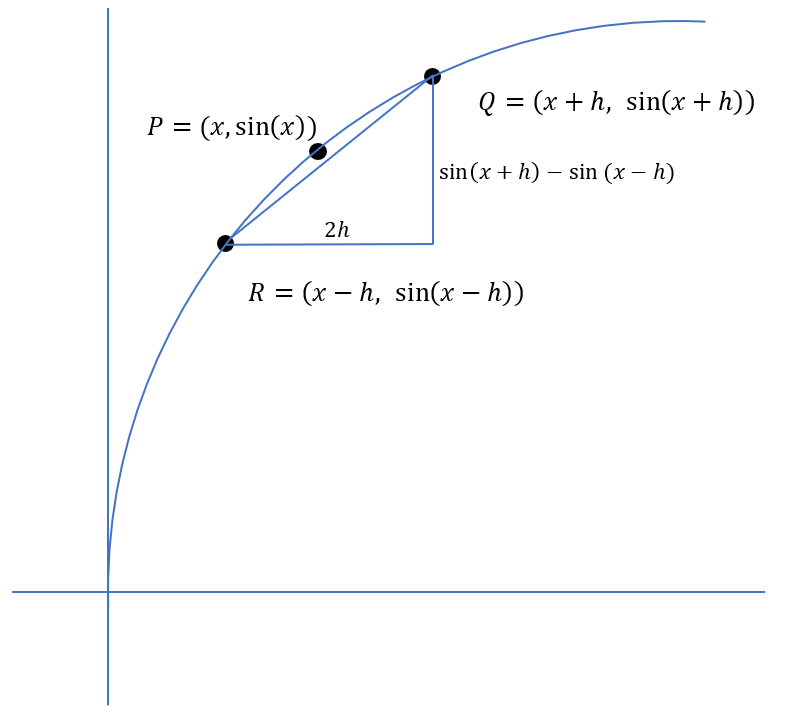
\includegraphics[width=\textwidth]{sinederivation1}}
\end{figure}
From first principles, we can say that:
\begin{equation*}
\frac{\mathrm{d}}{\mathrm{d}x}\left[\sin(x)\right]=\lim_{h\to0}\left[\frac{\sin(x+h)-\sin(x-h)}{2h}\right]
\end{equation*}
and using compound angle formulae (section \ref{compoundangleformulae}), we have:
\begin{equation*}
\sin(x+h)-\sin(x-h)=2\cos(x)\sin(h)
\end{equation*}
Thus:
\begin{equation*}
\frac{\mathrm{d}}{\mathrm{d}x}\left[\sin(x)\right]=\lim_{h\to0}\left[\frac{2\cos(x)\sin(h)}{2h}\right]=\lim_{h\to0}\left[\frac{\cos(x)\sin(h)}{h}\right]
\end{equation*}
\begin{figure}[H]
\centering
\scalebox{.95}{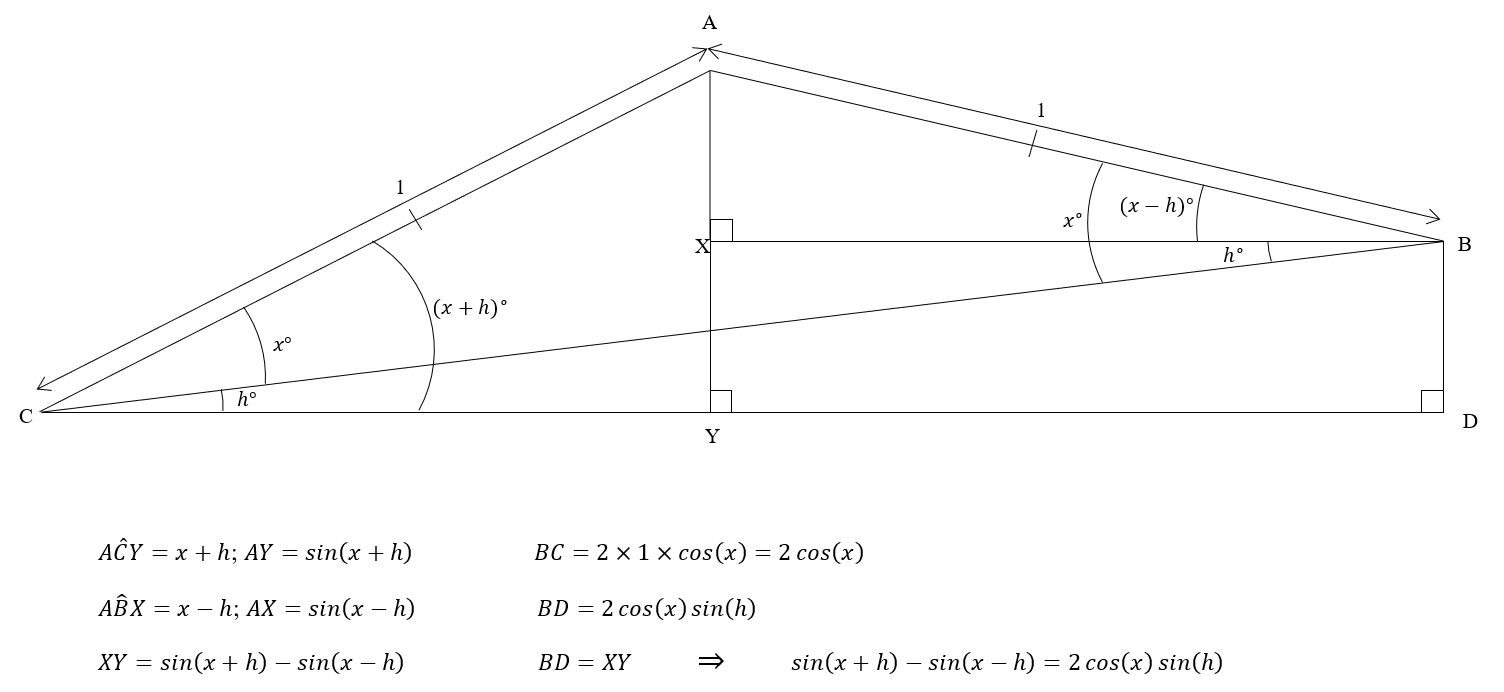
\includegraphics[width=\textwidth]{sinederivation2}}
\end{figure}
and since $\cos(x)$ is fixed:
\begin{equation*}
\lim_{h\to0}\left[\frac{\cos(x)\sin(h)}{h} \right]=\cos(x)\times\lim_{h\to0}\left[ \frac{\sin(h)}{h}\right]
\end{equation*}
Again requiring radians to be used, this limit evaluates to 1 when working in radians\footnote{This limit evaluates to $\frac{\pi}{180}$ when working in degrees}, so we recover:
\begin{equation*}
\frac{\mathrm{d}}{\mathrm{d}x}\left[ \sin(x) \right]=\cos(x)
\end{equation*}
To then find the derivative of $\cos(x)$, we can use a trick involving the chain rule. $\cos(x)$ can be written as a composite function, with
\begin{equation*}
\cos(x)=\sin\left( \frac{\pi}{2}-x \right)
\end{equation*}
Then taking the derivative of both sides, and applying the chain rule;
\begin{align*}
\frac{\mathrm{d}}{\mathrm{d}x}\left[ \cos(x) \right] &= \frac{\mathrm{d}}{\mathrm{d}x}\left[ \sin\left( \frac{\pi}{2}-x \right) \right] \\
&=\cos\left( \frac{\pi}{2}-x \right)\cdot\frac{\mathrm{d}}{\mathrm{d}x}\left[ \frac{\pi}{2}-x \right] \\
&=-\cos\left( \frac{\pi}{2}-x \right) \\
&=-\sin(x)
\end{align*}
Therefore;
\begin{equation*}
\frac{\mathrm{d}}{\mathrm{d}x}\left[ \cos(x) \right]=-\sin(x)
\end{equation*}
\vspace{0.5cm}


\subsection{Derivatives of standard and reciprocal trigonometric functions}
\begin{itemize}
\item A Level M Year 2 \hspace{1cm} \phantom{ AS / } Pages 185 -- 195
\end{itemize} \par

Here is a list of the derivatives of standard and reciprocal trigonometric functions. The reciprocal functions can be obtained by applying the quotient rule (section \ref{quotientrule}).

\begin{center}
\begin{tblr}{|[.75pt]|c|c||[.75pt]}
\hline[1.25pt]
$f(x)$ & $\frac{\mathrm{d}}{\mathrm{d}x}\left[ f(x) \right]$ \\ \hline[.75pt]
$\sin(x)$ & $\cos(x)$ \\ \hline
$\cos(x)$ & $-\sin(x)$ \\ \hline
$\tan(x)$ & $\sec^{2}(x)$ \\ \hline
$\cosec(x)$ & $-\cosec(x)\cot(x)$ \\ \hline
$\sec(x)$ & $\sec(x)\tan(x)$ \\ \hline
$\cot(x)$ & $-\cosec^{2}(x)$ \\ \hline[1pt]
\end{tblr}
\end{center}

\vspace{0.5cm}


\subsection{Derivatives of the inverse trigonometric functions}
\label{inversetrigderivatives}
\begin{itemize}
\item A Level FM Year 2 \hspace{1cm} \phantom{AS /} Pages 152 -- 157
\end{itemize} \par
The derivatives of inverse trigonometric functions can be found using implicit differentiation (see section \ref{implicitdifferentiation}). A brief demonstration for the derivatives of $\arccos$, $\arcsin$, and $\arctan$ follow. 
\subsubsection*{arcsin}
\vspace{-0.8cm}
\begin{flalign*}
y&=\arcsin(x) && \\
x&=\sin(y) && \\
1&=\cos(y)\frac{\mathrm{d}y}{\mathrm{d}x} && \\
\frac{\mathrm{d}y}{\mathrm{d}x}&=\frac{1}{\cos(y)}=\frac{1}{\pm\sqrt{1-\sin^{2}(y)}}=\frac{1}{\pm\sqrt{1-x^{2}}} && \\
&\text{\small{ Gradient always positive, so: }} && \\
\frac{\mathrm{d}y}{\mathrm{d}x}&=\frac{1}{\sqrt{1-x^{2}}} && \\
\end{flalign*}
\subsubsection*{arccos}
\vspace{-0.8cm}
\begin{flalign*}
y&=\arccos(x) && \\
x&=\cos(y) && \\
1&=-\sin(y)\frac{\mathrm{d}y}{\mathrm{d}x} && \\
\frac{\mathrm{d}y}{\mathrm{d}x}&=\frac{-1}{\sin(y)}=\frac{-1}{\pm\sqrt{1-\cos^{2}(y)}}=\frac{1}{\mp\sqrt{1-x^{2}}} && \\
&\text{\small{ Gradient always negative, so: }} && \\
\frac{\mathrm{d}y}{\mathrm{d}x}&=-\frac{1}{\sqrt{1-x^{2}}} && \\
\end{flalign*}
\subsubsection*{arctan}
\vspace{-0.8cm}
\begin{flalign*}
y&=\arctan(x) && \\
x&=\tan(y) && \\
1&=\sec^{2}(y)\frac{\mathrm{d}y}{\mathrm{d}x} && \\
\frac{\mathrm{d}y}{\mathrm{d}x}&=\frac{1}{\sec^{2}(y)}=\frac{1}{1+\tan^{2}(y)}=\frac{1}{1+x^{2}} &&
\end{flalign*}

\subsection{Integrals using trigonometric identities}
\begin{itemize}
\item A Level M Year 2 \hspace{1cm} \phantom{ AS / } Pages 234 -- 239
\end{itemize}
Integrals containing powers of trigonometric functions can be dealt with by using identities involving these functions. A general integral involving powers of sines and cosines\footnote{The other Pythagorean identities can be used for integrals involving powers of the tangent and secant, or powers of the cotangent and cosecant} has the form
\begin{equation*}
\int \sin^{m}(x)\cos^{n}(x)\,\mathrm{d}x
\end{equation*}
and has three main cases:
\begin{itemize}
\item[Case 1:] Power of sine is odd and positive
\item[] For an odd powered sine term, take off a $\sin(x)$ and put it at the end
\begin{equation*}
\int \sin^{2n+1}(x)\cos^{m}(x)\,\mathrm{d}x=\int\sin^{2n}(x)\cos^{m}(x)\times\sin(x)\,\mathrm{d}x
\end{equation*}
Then, turn every remaining even power of sine into cosines using a trigonometric identity.
\begin{equation*}
\int \sin^{2n}(x)\cos^{m}(x)\times\sin(x)\,\mathrm{d}x=\int \left( 1-\cos^{2}(x) \right)^{n}\cos^{m}(x)\times\sin(x)\,\mathrm{d}x
\end{equation*}
Now, we can simply expand out the brackets, and since the remaining sine term can be treated as the result of a chain rule, the integral can be done by inspection, as it is essentially a polynomial in $\cos(x)$.
\newpage
\item[Case 2:] Power of cosine is odd and positive
\item[] This is essentially the same as for Case 1. For an odd powered cosine term, take off a $\cos(x)$ and put it at the end
\begin{equation*}
\int \sin^{n}(x)\cos^{2m+1}(x)\,\mathrm{d}x=\int\sin^{n}(x)\cos^{2m}(x)\times\cos(x)\,\mathrm{d}x
\end{equation*}
Then, turn every remaining even power of cosine into sines using a trigonometric identity.
\begin{equation*}
\int \sin^{n}(x)\cos^{2m}(x)\times\cos(x)\,\mathrm{d}x=\int \sin^{n}(x)\left( 1-\sin^{2}(x) \right)^{m}\times\cos(x)\,\mathrm{d}x
\end{equation*}
Now, we can simply expand out the brackets, and since the remaining cosine term can be treated as the result of a chain rule, the integral can be done by inspection, as it is essentially a polynomial in $\sin(x)$.
\item[Case 3:] Powers of both sine and cosine are even and positive
\item[] In this case, we need to use half-angle trigonometric identities to convert the integrand into \emph{odd} powers of cosines.
\begin{align*}
\sin^{2}(x)&\frac{1-\cos(2x)}{2} \\
\cos^{2}(x)&=\frac{1+\cos(2x)}{2}
\end{align*}
So, for example,
\begin{align*}
\int\sin^{2}(x)\cos^{2}(x)\,\mathrm{d}x&=\int\left[ \sin^{2}(x)\frac{1-\cos(2x)}{2} \right]\left[ \cos^{2}(x)\frac{1+\cos(2x)}{2} \right]\,\mathrm{d}x \\
&=\frac{1}{4}\int 1-\cos^{2}(2x)\,\mathrm{d}x \\
&=\frac{1}{4}\int 1-\frac{1+\cos(4x)}{2}\,\mathrm{d}x \\
&=\frac{1}{8}\int 2-1-\cos(4x)\,\mathrm{d}x \\
&=\frac{1}{8}\int 1-\cos(4x)\,\mathrm{d}x \\
&=\frac{1}{8}x-\frac{1}{32}\sin(4x)+c
\end{align*}
\end{itemize}
\vspace{0.5cm}


\subsection{Integrals via inverse trigonometric functions: Standard results}
\begin{itemize}
\item A Level FM Year 2 \hspace{1cm} \phantom{AS /} Pages 152 -- 157
\end{itemize} \par
This is the origin of some of the integrals in the section on standard integrals, in section \ref{usefulintegrals}. They come from combining the results of the inverse trigonometric functions (section \ref{inversetrigderivatives}) with the chain rule (section \ref{chainrule}). Once again, these are in the formula booklet, so do not necessarily need to be memorised, but they should be recognised.

\begin{gather*}
\int\frac{1}{\sqrt{a^{2}-x^{2}}}\,\mathrm{d}x=\arcsin\left( \frac{x}{a} \right) + c \\
 \\
\int\frac{1}{a^{2}+x^{2}}\,\mathrm{d}x=\frac{1}{a}\arctan\left( \frac{x}{a} \right) + c \\
\end{gather*}

\vspace{0.5cm}



\clearpage
\section{Vectors and Matrices}
\vspace{0.5cm}

\subsection{Vector notation}
\begin{itemize}
\item A Level M AS / Year 1 \hspace{1cm} \phantom{ } Pages 220 -- 244
\end{itemize} \par
An arrow above two letters, such as
\begin{equation*}
\overrightarrow{AB}
\end{equation*}
 denotes the vector that takes point $A$ to point $B$. Also note:
\begin{equation*}
\overrightarrow{AB}+\overrightarrow{BC}=\overrightarrow{AC}
\end{equation*}
The vector ascribed to a variable, for example $r$ can be shown to be a vector quantity in three ways. When in print, vectors are commonly denoted in bold. However it is quite hard to handwrite bold font. So, we can either underline the character, or put an arrow over the top. All three are equivalent ways of writing the same vector quantity.


\begin{figure}[H]
\centering
\begin{subfigure}[c]{0.59\textwidth}
\begin{center}
\begin{tblr}{|[.75pt]|c|c|c||[.75pt]}
\hline[1.25pt]
Bold font & Underline & Arrow \\ \hline
$\boldsymbol{r}$ & $\underline{r}$ & $\vec{r}$ \\ \hline[1pt]
\end{tblr}
\end{center}
\end{subfigure}
\hfill
\begin{subfigure}[c]{0.39\textwidth}
\centering
\begin{equation*}
\boldsymbol{r} = \underline{r} = \vec{r} = \begin{bmatrix}x\\y\\z\end{bmatrix}
\end{equation*}
\end{subfigure}
\end{figure}
\begin{itemize}
\item[Note:] Normalised vectors (vectors of length 1) are often written with a `hat' above them
\end{itemize}
\begin{gather*}
\hat{\boldsymbol{r}}=\hat{\underline{r}}=\hat{\vec{r}}=\frac{1}{\sqrt{x^{2}+y^{2}+z^{2}}}\begin{bmatrix}x\\y\\z\end{bmatrix} \\
\boldsymbol{r}=|\boldsymbol{r}|\hat{\boldsymbol{r}} \hspace{1.5cm} \hat{\boldsymbol{r}}=\frac{1}{|\boldsymbol{r}|}\boldsymbol{r}
\end{gather*}
\vspace{0.5cm}


\subsection{The vector equation of a line}
\begin{itemize}
\item A Level FM AS / Year 1 \hspace{1cm} Pages 33 -- 39
\item A Level FM AS / Year 1 \hspace{1cm} Pages 45 -- 48
\end{itemize} \par
A line can be defined in terms of vectors or Cartesian coordinates. the form
\begin{equation*}
\boldsymbol{r}=\boldsymbol{a}+\lambda\boldsymbol{b}
\end{equation*}
gives the position vector of a point on the line, where
\begin{itemize}
\item[-]$\boldsymbol{a}$ is the position vector of a fixed point on the line
\vspace{-0.25cm}
\item[-]$\boldsymbol{b}$ is the vector which maps $\boldsymbol{a}$ to another point on the line
\vspace{-0.25cm}
\item[-]$\boldsymbol{r}$ is a general point on the line
\vspace{-0.25cm}
\item[-]$\lambda$ is a scalar variable coefficient
\end{itemize}

In 2D, lines must be either \underline{parallel}, or \underline{intersecting}, unless they are the same line.

In 3D, lines can be either \underline{parallel}, or \underline{non-parallel and intersecting}, or \underline{non-parallel and non-intersecting} (skew), unless they are the same line.
\vspace{0.5cm}


\subsection{Cartesian form of the equations of a line in 3D}
\begin{itemize}
\item A Level FM AS / Year 1 \hspace{1cm} Pages 39 -- 45
\end{itemize} \par
A line can also be defined in terms of Cartesian coordinates. This can be done by rearranging the vector equation.
\begin{equation*}
\begin{bmatrix}x\\y\\z\end{bmatrix}=\boldsymbol{r}=\begin{bmatrix}a\\b\\c\end{bmatrix}+\lambda\begin{bmatrix}f\\g\\h\end{bmatrix}
\end{equation*}
\begin{flalign*}
\Rightarrow x&=a+f\lambda & \hspace{-1cm}\Leftrightarrow \hspace{1cm}& \lambda=\frac{x-a}{f} && \\
\Rightarrow y&=b+g\lambda & \hspace{-1cm}\Leftrightarrow \hspace{1cm}& \lambda=\frac{y-b}{g} && \\
\Rightarrow z&=c+h\lambda & \hspace{-1cm}\Leftrightarrow \hspace{1cm}& \lambda=\frac{z-c}{h} &&
\end{flalign*} \newline \par
Therefore, the Cartesian form of the line is
\begin{equation*}
\frac{x-a}{f}=\frac{y-b}{g}=\frac{z-c}{h}(=\lambda)
\end{equation*}
This form can be easily rearranged to give $x$, $y$, and $z$ in terms of $\lambda$, from which the vector equation may be obtained.
\vspace{0.5cm}

\newpage
\subsection{The scalar product (or dot product)}
\begin{itemize}
\item A Level FM AS / Year 1 \hspace{1cm} Pages 48 -- 56
\end{itemize} \par
The scalar product of two vectors is an operation which takes two vectors and returns a scalar, hence the name `scalar' product. This `derivation' is not necessary to remember, but the final result is an important one.
\begin{figure}[H]
\centering
\begin{subfigure}[b]{0.85\textwidth}
\scalebox{.85}{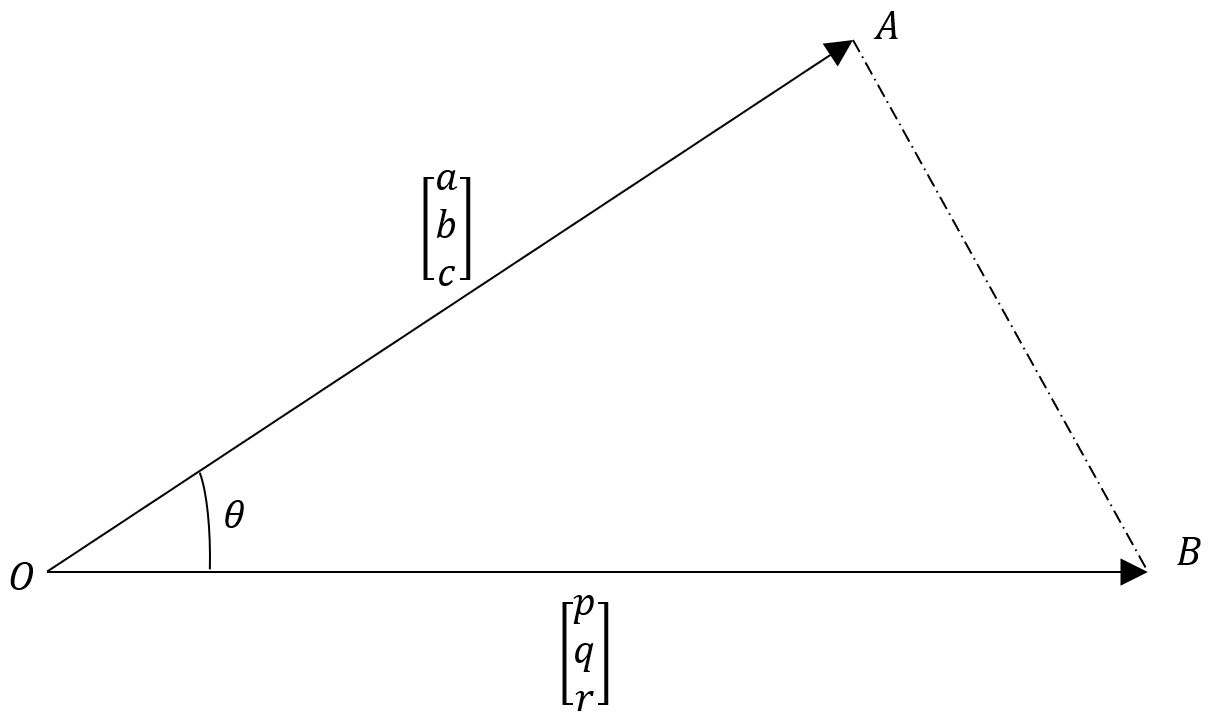
\includegraphics[width=\textwidth]{scalarproduct}}
\end{subfigure}
\end{figure}
Using the cosine rule, we obtain:
\begin{equation*}
\left( \overrightarrow{AB} \right)^{2}=\left( \overrightarrow{OA} \right)^{2}+\left( \overrightarrow{OB} \right)^{2}-2\cdot\left( \overrightarrow{OA} \right)\cdot\left( \overrightarrow{OB} \right)\cdot\cos(\theta)
\end{equation*}

And,
\begin{equation*}
\overrightarrow{AB}=\overrightarrow{OB}-\overrightarrow{OA}=\begin{bmatrix} p-a \\ q-b \\ r-c \end{bmatrix}
\end{equation*}

Therefore:
\begin{equation*}
\begin{bmatrix} p-a \\ q-b \\ r-c \end{bmatrix}^{2}=\begin{bmatrix} a \\ b \\ c \end{bmatrix}^{2}+\begin{bmatrix} p \\ q \\ r \end{bmatrix}^{2}-2\begin{bmatrix} a \\ b \\ c \end{bmatrix}\begin{bmatrix} p \\ q \\ r \end{bmatrix}\cos(\theta)
\end{equation*}

We can expand this, by taking the magnitude (represented by $|\cdot|$) of each of the vectors involved:
\small
\begin{multline*}
(p-a)^{2}+(q-b)^{2}+(r-c)^{2}=\\ \left( a^{2} +b^{2} +c^{2} \right) + \left( p^{2} +q^{2} +r^{2} \right) - 2\sqrt{ a^{2} +b^{2} +c^{2}}\sqrt{ p^{2} +q^{2} +r^{2}}\cos(\theta)
\end{multline*}
\begin{multline*}
p^{2}-2ap+a^{2}+q^{2}-2qb+b^{2}+r^{2}-2cr+c^{2}=\\a^{2}+b^{2}+c^{2}+p^{2}+q^{2}+r^{2}-2\sqrt{ a^{2} +b^{2} +c^{2}}\sqrt{ p^{2} +q^{2} +r^{2}}\cos(\theta)
\end{multline*}
\begin{multline*}
\cancel{p^{2}}+\cancel{a^{2}}+\cancel{q^{2}}+\cancel{b^{2}}+\cancel{r^{2}}+\cancel{c^{2}}-2(ap+bq+cr)=\\\cancel{a^{2}}+\cancel{b^{2}}+\cancel{c^{2}}+\cancel{p^{2}}+\cancel{q^{2}}+\cancel{r^{2}}-2\sqrt{ a^{2} +b^{2} +c^{2}}\sqrt{ p^{2} +q^{2} +r^{2}}\cos(\theta)
\end{multline*}
\normalsize
Thus:
\begin{equation*}
\cos(\theta)=\frac{(ap+br+cq)}{\sqrt{ a^{2} +b^{2} +c^{2}}\sqrt{ p^{2} +q^{2} +r^{2}}}=\frac{(ap+br+cq)}{\left|\begin{bmatrix} a \\ b \\ c \end{bmatrix}\right|\times\left|\begin{bmatrix} p \\ q \\ r \end{bmatrix}\right|}
\end{equation*}
This rearranges to give
\begin{equation*}
\left|\begin{bmatrix} a \\ b \\ c \end{bmatrix}\right|\times\left|\begin{bmatrix} p \\ q \\ r \end{bmatrix}\right|\times \cos(\theta)=ap+br+cq
\end{equation*}

We can therefore define the \emph{scalar product}, or \emph{dot product} of two vectors $\boldsymbol{x}$ and $\boldsymbol{y}$ to be
\begin{equation*}
\boldsymbol{x}\cdot\boldsymbol{y}=\begin{bmatrix} a \\ b \\ c \end{bmatrix}\cdot\begin{bmatrix} p \\ q \\ r \end{bmatrix}=ap+bq+cr
\end{equation*}

$\boldsymbol{x}$ and $\boldsymbol{y}$ are both vectors, however their scalar product, denoted by a `dot', $(ap+bq+cr)$ is a scalar. The scalar product theorem is defined as:
\begin{equation*}
\boldsymbol{x}\cdot\boldsymbol{y}=|\boldsymbol{x}||\boldsymbol{y}|\cos(\theta)
\end{equation*}
An important result is that if the two vectors are perpendicular, the angle between them is $90^{\circ}$, and $\cos(90)=0$, so the scalar product is 0. On the other hand, if the two vectors are the same, then the angle between them is $0^{\circ}$, and $\cos(0)=1$, so the scalar product is the square of the magnitude of the vector.
\vspace{0.5cm}


\subsection{The vector product (or cross product)}
\label{crossproduct}
\begin{itemize}
\item A Level FM AS / Year 1 \hspace{1cm} Pages 56 -- 61
\end{itemize} \par
The vector product of two vectors is an operation which takes two vectors and returns another vector, which is perpendicular to both the original vectors. Again, the derivation is unnecessary to remember, but the final results are very important.\newline\par

We want to find
\begin{equation*}
\begin{bmatrix}x\\y\\z\end{bmatrix}\perp\begin{bmatrix}a\\b\\c\end{bmatrix},\begin{bmatrix}p\\q\\r\end{bmatrix}
\end{equation*}
From the scalar product theorem, for perpendicular vectors, we require
\begin{align*}
\begin{bmatrix}x\\y\\z\end{bmatrix}\cdot\begin{bmatrix}a\\b\\c\end{bmatrix}&=0 & \begin{bmatrix}x\\y\\z\end{bmatrix}\cdot\begin{bmatrix}p\\q\\r\end{bmatrix}&=0 \\
& & & \\
ax+by+cz&=0 & px+qy+rz&=0 \\
arx+bry+crz&=0 & pcx+qcy+rcz&=0
\end{align*}
Therefore:
\begin{flalign*}
(arx+bry+crz)-(pcx+qcy+rcz)&=0 && \\
(arx+bry-cpx-qcy)&=0 && \\
(ar-cp)x+(br-cq)y&=0 && \\
(br-cq)y&=-(ar-cp)x && \\
&=(cp-ar)x  &&
\end{flalign*}

Let $x=(br-cq)$ and let $y=(cp-ar)$. Substituting this back in,
\begin{flalign*}
a(br-cq)+b(cp-ar)+cz&=0 && \\
\cancel{abr}-acq+bcp-\cancel{bar}&=-cz && \\
c(bp-aq)&=-cz && \\
& && \\
z&=(aq-bp)
\end{flalign*}
So,
\begin{equation*}
\begin{bmatrix}x\\y\\z\end{bmatrix}=\begin{bmatrix}br-cq\\cp-ar\\aq-bp\end{bmatrix}
\end{equation*}
and so we define the cross product:
\begin{equation*}
\begin{bmatrix}a\\b\\c\end{bmatrix}\times\begin{bmatrix}p\\q\\r\end{bmatrix}=\begin{bmatrix}br-cq\\cp-ar\\aq-bp\end{bmatrix}
\end{equation*}

$\boldsymbol{x}$ and $\boldsymbol{y}$ are both vectors, and their vector product, denoted by a `cross', is a vector. The vector product theorem is defined as:
\begin{equation*}
\boldsymbol{x}\times\boldsymbol{y}=|\boldsymbol{x}||\boldsymbol{y}|\sin(\theta)
\end{equation*} 

There are a couple of tricks to remembering how the cross product evaluates. Here is one, but by no means the only way of doing it. \newline \par

\noindent Take the determinant of the $3\times3$ matrix:
\begin{equation*}
\begin{bmatrix} \hat{\boldsymbol{\imath}} & \hat{\boldsymbol{\jmath}} & \hat{\boldsymbol{k}} \\ a & b & c \\ p & q & r \end{bmatrix}
\end{equation*}
This can be done by multiplying the diagonals, and adding the right-diagonals (\textcolor{red}{red}, \textcolor{blue}{blue}\ and \textcolor{purple}{purple}), and subtracting the left-diagonals (\textcolor{cyan}{cyan}, \textcolor{magenta}{magenta}\ and \textcolor{orange}{orange}).
\begin{gather*}
\begin{bmatrix} \textcolor{red}{\hat{\boldsymbol{\imath}}} & \textcolor{blue}{\hat{\boldsymbol{\jmath}}} & \textcolor{purple}{\hat{\boldsymbol{k}}} \\ \textcolor{purple}{a} & \textcolor{red}{b} & \textcolor{blue}{c} \\ \textcolor{blue}{p} & \textcolor{purple}{q} & \textcolor{red}{r} \end{bmatrix}\hspace{3.5cm}\begin{bmatrix} \textcolor{cyan}{\hat{\boldsymbol{\imath}}} & \textcolor{magenta}{\hat{\boldsymbol{\jmath}}} & \textcolor{orange}{\hat{\boldsymbol{k}}} \\ \textcolor{magenta}{a} & \textcolor{orange}{b} & \textcolor{cyan}{c} \\ \textcolor{orange}{p} & \textcolor{cyan}{q} & \textcolor{magenta}{r} \end{bmatrix} \\
(br)\hat{\boldsymbol{\imath}}+(cp)\hat{\boldsymbol{\jmath}}+(aq)\hat{\boldsymbol{k}} \hspace{1.5cm} -(cq)\hat{\boldsymbol{\imath}}-(ar)\hat{\boldsymbol{\jmath}}-(bp)\hat{\boldsymbol{k}} 
\end{gather*}
This determinant evaluates as
\begin{equation*}
(br-cq)\hat{\boldsymbol{\imath}}+(cp-ar)\hat{\boldsymbol{\jmath}}+(aq-bp)\hat{\boldsymbol{k}}=\begin{bmatrix}br-cq\\cp-ar\\aq-bp\end{bmatrix}
\end{equation*}

The vectors $\boldsymbol{x}$, $\boldsymbol{y}$, and $\boldsymbol{x}\times\boldsymbol{y}$ form a right-handed set, with $\boldsymbol{x}$ as the index finger, $\boldsymbol{y}$ as the third finger, and $\boldsymbol{x}\times\boldsymbol{y}$ as the thumb. The direction of the thumb shows the direction of $\boldsymbol{x}\times\boldsymbol{y}$ relative to $\boldsymbol{x}$ and $\boldsymbol{y}$. \newline \par

\begin{itemize}
\item[Note:] Here are a couple of useful results, both of which are relatively easy to show by working through:\begin{gather*} \boldsymbol{x}\times\boldsymbol{y}=-\left( \boldsymbol{y}\times\boldsymbol{x} \right) \\ \boldsymbol{x}\times\boldsymbol{x}=\boldsymbol{0} \end{gather*}
\end{itemize}

\vspace{0.5cm}


\subsection{The vector product of unit vectors}

\begin{center}
\begin{tblr}{|[1pt]c|c|[1pt]c|c|c|[1pt]}
\hline[1pt]
\SetCell[r=2,c=2]{c} $\hat{\boldsymbol{u}}\times\hat{\boldsymbol{v}}$& & \SetCell[c=3]{c}$\hat{\boldsymbol{u}}$ & & \\ \hline
& & $\hspace{0.8cm}\hat{\boldsymbol{\imath}}\hspace{0.8cm}$ & $\hspace{0.8cm}\hat{\boldsymbol{\jmath}}\hspace{0.8cm}$ & $\hspace{0.8cm}\hat{\boldsymbol{k}}\hspace{0.8cm}$ \\ \hline[1pt]
\SetCell[r=3]{c} $\hat{\boldsymbol{v}}$ & $\hat{\boldsymbol{\imath}}$ & $\boldsymbol{0}$ & $-\boldsymbol{k}$ & $\hat{\boldsymbol{\jmath}}$ \\ \hline
& $\hspace{0.8cm}\hat{\boldsymbol{\jmath}}\hspace{0.8cm}$ & $\hat{\boldsymbol{k}}$ & $\boldsymbol{0}$ & $-\hat{\boldsymbol{\imath}}$ \\ \hline
& $\hspace{0.8cm}\hat{\boldsymbol{k}}\hspace{0.8cm}$ & $-\hat{\boldsymbol{\jmath}}$ & $\hat{\boldsymbol{\imath}}$ & $\boldsymbol{0}$ \\ \hline[1pt]
\end{tblr}
\end{center}
\vspace{0.5cm}


\subsection{The equation of a plane}
\begin{itemize}
\item A Level FM Year 2 \hspace{1cm} \phantom{AS /} Pages 72 -- 81
\end{itemize} \par
A plane in 3D space is defined by
\begin{equation*}
ax+by+cz=k
\end{equation*}
in its Cartesian form, where $a$, $b$, $c$, and $k$ are constants. \newline \par
The vector $\begin{bmatrix}a \\ b \\ c\end{bmatrix}$ is normal to the plane. Therefore, the plane can be expressed in vector form as well:
\begin{equation*}
\begin{bmatrix} x \\ y \\ z \end{bmatrix}\cdot\begin{bmatrix} a \\ b \\ c \end{bmatrix}=k
\end{equation*}

What information is necessary to define a plane? The following pieces of information are sufficient to define a plane, but the first two criteria require the cross-product (see section \ref{crossproduct}) to find the plane
\begin{itemize}
\item[-]3 non-collinear points that are on the plane
\item[-]1 point on the plane, and 2 non-parallel directions contained in the plane
\item[-]1 point and a vector normal to the plane
\end{itemize}
\vspace{0.5cm}

\subsection{Planes}
\begin{itemize}
\item A Level FM Year 2 \hspace{1cm} \phantom{AS /} Pages 72 -- 95
\end{itemize} \par
\begin{itemize}
\item[-] To find the angle between a line and a plane, find the angle between the line and the normal of the plane, and then subtract the result from $90^{\circ}$ / $\frac{\pi}{2}$.
\item[-] To find the poition of intersection between a line and plane, find $x$, $y$, $z$ in terms of $\lambda$ from the vector equation of the line, substitute into the equation of the plane and solve for $\lambda$, which can then be substituted back into the vector equation of the line to give the point of intersection
\item[-] To find the angle between two planes, this is the same as the angle between the normal vectors to each plane -- simply use the scalar product or cross product theorem on the two normal vectors to find the angle.
\item[-] To find the equation of a plane through three non-collinear points, first find two vectors in the plane (i.e. for points $A$, $B$, and $C$, the vectors $\overrightarrow{AB}$ and the vectors $\overrightarrow{AC}$ will do) and take their vector product, to find a vector normal to the plane. Substitute values of $x$, $y$, and $z$, to find the constant term of the equation.
\end{itemize}
\vspace{0.5cm}


\subsection{Geometric applications of the scalar and vector products}
\begin{itemize}
\item A Level FM Year 2 \hspace{1cm} \phantom{AS /} Pages 82 -- 95
\end{itemize} \par
Here are two applications of the scalar and vector product. These results are given in the formula booklet, so do not need to be memorised, but again, you should recognise them, and it is useful to know where they come from.
\subsubsection*{The distance of a point from a plane}
$A$ and $N$ are points (with vectors $\boldsymbol{a}$ and $\boldsymbol{n}$ respectively) contained within the plane defined by $\boldsymbol{r}\cdot\boldsymbol{n}=p$. $B$ is a point in space (with vector $\boldsymbol{b}$), and $\boldsymbol{n}$ is a vector normal to the plane.
\begin{figure}[H]
\centering
\scalebox{.65}{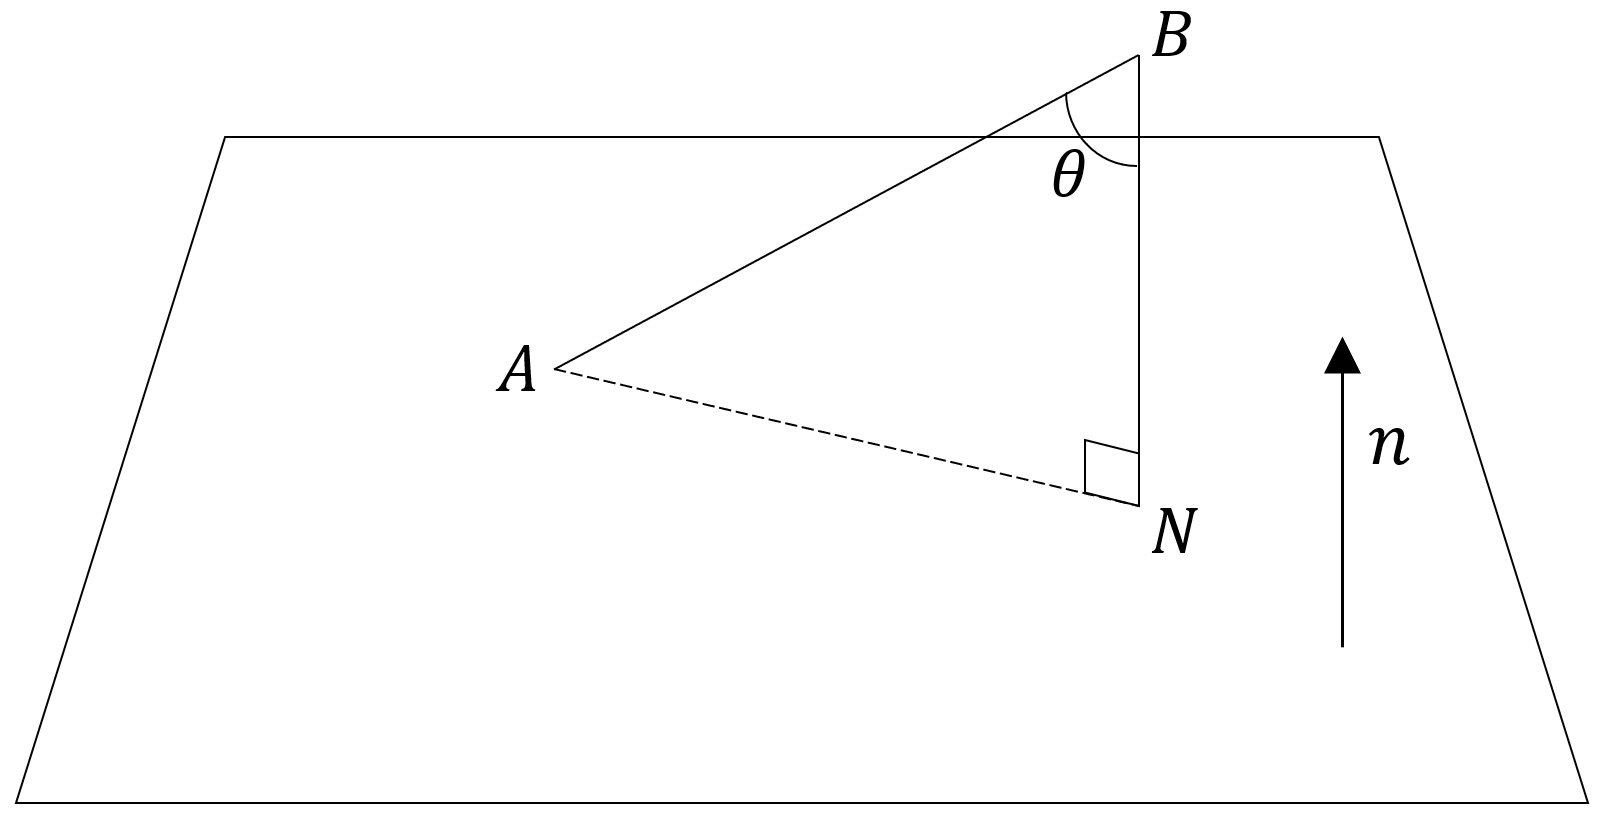
\includegraphics[width=\textwidth]{pointfromplane}}
\end{figure}
$\overrightarrow{AB}=\boldsymbol{b}-\boldsymbol{a}$, and from simple geometry,
\begin{equation*}
\left|\overrightarrow{BN}\right|=|\boldsymbol{b}-\boldsymbol{a}|\cos(\theta)
\end{equation*}
We can then use the scalar product theorem and rearrange:
\begin{align*}
(\boldsymbol{b}-\boldsymbol{a})\cdot\boldsymbol{n}&=|\boldsymbol{b}-\boldsymbol{a}||\boldsymbol{n}|\cos(\theta) \\
\frac{\left| (\boldsymbol{b}-\boldsymbol{a})\cdot\boldsymbol{n} \right|}{|\boldsymbol{n}|}&=|\boldsymbol{b}-\boldsymbol{a}|\cos(\theta)=\left|\overrightarrow{BN}\right|
\end{align*}
\scriptsize
Since $0\leq\theta\leq\frac{\pi}{2}$, $0\leq\cos(\theta)\leq1$. Therefore, $|\boldsymbol{b}-\boldsymbol{a}|\cos(\theta)>0$, so the modulus of $(\boldsymbol{b}-\boldsymbol{a})\cdot\boldsymbol{n}$ must be taken.
\normalsize

\begin{equation*}
\left| (\boldsymbol{b}-\boldsymbol{a})\cdot\boldsymbol{n} \right|=\left| \boldsymbol{b}\cdot\boldsymbol{n}-\boldsymbol{a}\cdot\boldsymbol{n} \right|
\end{equation*}
And recall that $\boldsymbol{a}$ is an arbitrary point in the plane. using the fact that $\boldsymbol{a}\cdot\boldsymbol{n}=p$, we can substitute in:
\begin{equation*}
\left| (\boldsymbol{b}-\boldsymbol{a})\cdot\boldsymbol{n} \right|=\left| \boldsymbol{b}\cdot\boldsymbol{n}-p \right|
\end{equation*}
Therefore
\begin{equation*}
\left|\overrightarrow{BN}\right|=\frac{\left| \boldsymbol{b}\cdot\boldsymbol{n}-p \right|}{|\boldsymbol{n}|}
\end{equation*}


\vspace{0.5cm}
\subsubsection*{The distance of a point from a line}
$A$ and $N$ are points (with vectors $\boldsymbol{a}$ and $\boldsymbol{n}$ respectively) contained within the line defined by $\boldsymbol{r}=\boldsymbol{a}+\lambda\boldsymbol{n}$. $\overrightarrow{NB}$ is such that it is perpendicular to the line. $B$ is a point in space (with vector $\boldsymbol{b}$), and $\boldsymbol{n}$ is a vector parallel to the line.
\begin{figure}[H]
\centering
\scalebox{.65}{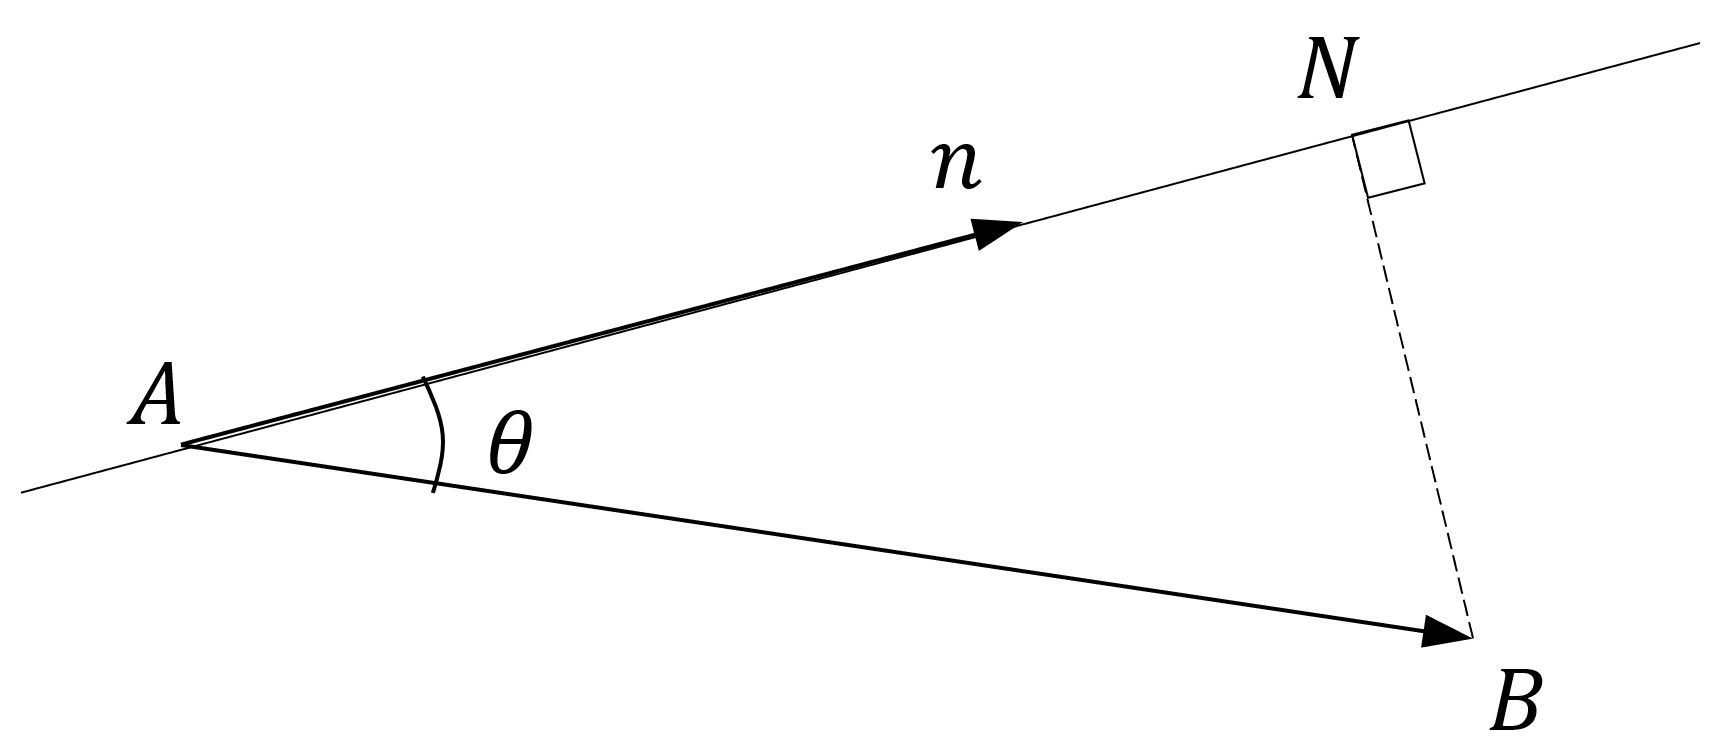
\includegraphics[width=\textwidth]{pointfromline}}
\end{figure}
$\overrightarrow{AB}=\boldsymbol{b}-\boldsymbol{a}$, and from simple geometry,
\begin{equation*}
\left|\overrightarrow{BN}\right|=|\boldsymbol{b}-\boldsymbol{a}|\sin(\theta)
\end{equation*}
We can then use the vector product theorem and rearrange:
\begin{align*}
(\boldsymbol{b}-\boldsymbol{a})\times\boldsymbol{n}&=|\boldsymbol{b}-\boldsymbol{a}||\boldsymbol{n}|\sin(\theta) \\
\frac{\left| (\boldsymbol{b}-\boldsymbol{a})\times\boldsymbol{n} \right|}{|\boldsymbol{n}|}&=|\boldsymbol{b}-\boldsymbol{a}|\sin(\theta)=\left|\overrightarrow{BN}\right|
\end{align*}
\scriptsize
Since $0\leq\theta\leq\frac{\pi}{2}$, $0\leq\sin(\theta)\leq1$. Therefore, $|\boldsymbol{b}-\boldsymbol{a}|\sin(\theta)>0$, so the modulus of $(\boldsymbol{b}-\boldsymbol{a})\times\boldsymbol{n}$ must be taken.
\normalsize

\subsubsection*{The distance of a point from a line in 2D}
Consider a line defined by
\begin{equation*}
ax+by=c
\end{equation*}
and the point $(x_{1},y_{1})$ in the $x$--$y$ plane, embedded in 3D space. \newline \par

The axis intercepts are $\left(\frac{c}{a},0,0\right)$ and $\left(0,\frac{c}{b},0\right)$. Therefore a vector equation of the line is given by
\begin{equation*}
\boldsymbol{r}=\begin{bmatrix} \frac{c}{a} \\ 0 \\ 0 \end{bmatrix}+\lambda\begin{bmatrix} \frac{c}{a} \\ -\frac{c}{b} \\ 0 \end{bmatrix}
\end{equation*}
Hence the distance of a point $\begin{bmatrix}x_{1} \\ y_{1} \\ 0 \end{bmatrix}$ from the line is
\small
\begin{align*}
\frac{\left| (\boldsymbol{b}-\boldsymbol{a})\times\boldsymbol{n} \right|}{|\boldsymbol{n}|}&=\frac{\left| \left(\begin{bmatrix}x_{1} \\ y_{1} \\ 0 \end{bmatrix}-\begin{bmatrix} \frac{c}{a} \\ 0 \\ 0 \end{bmatrix}\right)\times\begin{bmatrix} \frac{c}{a} \\ -\frac{c}{b} \\ 0 \end{bmatrix} \right|}{\left|\begin{bmatrix} \frac{c}{a} \\ -\frac{c}{b} \\ 0 \end{bmatrix}\right|}&=\frac{\left| \begin{bmatrix}x_{1}-\frac{c}{a} \\ y_{1} \\ 0 \end{bmatrix}\times\begin{bmatrix} \frac{c}{a} \\ -\frac{c}{b} \\ 0 \end{bmatrix} \right|}{\left|\begin{bmatrix} \frac{c}{a} \\ -\frac{c}{b} \\ 0 \end{bmatrix}\right|} \\
&=\frac{\left| \begin{bmatrix}0 \\ 0 \\ -\frac{x_{1}c}{b}+\frac{c^{2}}{ab}-\frac{y_{1}c}{a} \end{bmatrix} \right|}{\left|\begin{bmatrix} \frac{c}{a} \\ -\frac{c}{b} \\ 0 \end{bmatrix}\right|} &=\frac{\left| \begin{bmatrix}0 \\ 0 \\ \frac{c\left( c-x_{1}a-y_{1}b \right)}{ab} \end{bmatrix} \right|}{\left|\begin{bmatrix} \frac{c}{a} \\ -\frac{c}{b} \\ 0 \end{bmatrix}\right|} \\ 
&=\frac{\sqrt{\frac{c^{2}\left( c-x_{1}a-y_{1}b \right)^{2}}{(ab)^{2}}}}{\sqrt{\left( \frac{c}{a} \right)^{2} + \left( \frac{c}{b} \right)^{2}}} &=\frac{\frac{c}{ab}\sqrt{\left( c-x_{1}a-y_{1}b \right)^{2}}}{\frac{c}{ab}\sqrt{a^{2}+b^{2}}} \\
&=\frac{\left| c-x_{1}a-y_{1}b \right|}{\sqrt{a^{2}+b^{2}}} &=\frac{\left| x_{1}a+y_{1}b-c \right|}{\sqrt{a^{2}+b^{2}}}
\end{align*}
\normalsize
\vspace{0.5cm}


\subsection{The volume of a parallelepiped and the scalar triple product}
\begin{figure}[H]
\centering
\scalebox{.5}{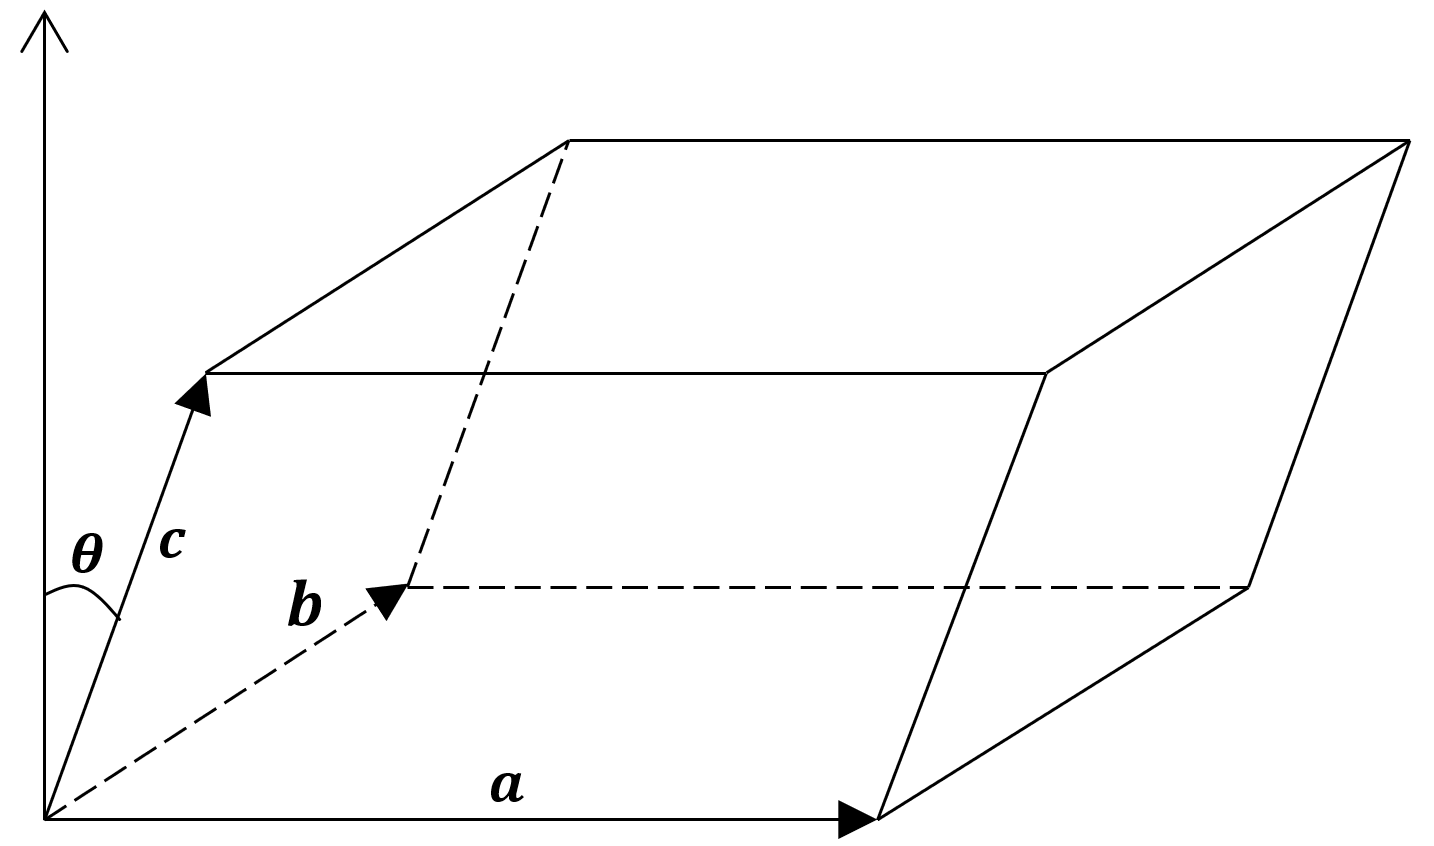
\includegraphics[width=\textwidth]{parallelepiped}}
\end{figure}
For a parallelepiped defined by the vectors $\boldsymbol{a}$, $\boldsymbol{b}$, and $\boldsymbol{c}$, the base area is defined by $\left|\boldsymbol{a}\times\boldsymbol{b}\right|$, and the perpendicular height is $\left|\boldsymbol{c}\right|\cos(\theta)$. \newline \par

Therefore the volume of the parallelepiped is
\begin{equation*}
\left|\boldsymbol{a}\times\boldsymbol{b}\right|\cdot\left|\boldsymbol{c}\right|\cos(\theta)=(\boldsymbol{a}\times\boldsymbol{b})\cdot\boldsymbol{c}
\end{equation*}
This is called the \emph{scalar triple product} of the vectors $\boldsymbol{a}$, $\boldsymbol{b}$, and $\boldsymbol{c}$. The result gives the signed volume of the parallelepiped spanned by $\boldsymbol{a}$, $\boldsymbol{b}$, and $\boldsymbol{c}$. So, in the case of a $3\times3$ matrix, this gives the volume scale factor of the unit cube, if $\boldsymbol{a}$, $\boldsymbol{b}$, and $\boldsymbol{c}$ are the three vectors that comprise the matrix. \newline \par

The scalar triple product has a cyclic property;
\begin{equation*}
\boldsymbol{c}\cdot(\boldsymbol{a}\times\boldsymbol{b})\equiv\boldsymbol{b}\cdot(\boldsymbol{c}\times\boldsymbol{a})\equiv\boldsymbol{a}\cdot(\boldsymbol{b}\times\boldsymbol{c})
\end{equation*}
since the scalar triple product is invariant under a circular shift of the vectors. \newline\par

$\boldsymbol{a}\cdot(\boldsymbol{b}\times\boldsymbol{c})$ is positive when $\boldsymbol{a}$, $\boldsymbol{b}$, and $\boldsymbol{c}$ form a right - handed set, and negative when $\boldsymbol{a}$, $\boldsymbol{b}$, and $\boldsymbol{c}$ form a left - handed set.
\vspace{0.5cm}
\newpage
\subsection{Configurations of three planes in three dimensions}
\begin{itemize}
\item A Level FM Year 2 \hspace{1cm} \phantom{AS /} Pages 104 -- 110
\end{itemize} \par
There are eight possible configurations of three planes in three dimensions. Given three planes, you should be able to establish which configuration they fall into, and find the point, line, or plane of solutions. An example system of planes / equations for each of the eight configuration is given in section \ref{planesexamples}

\begin{center}
\small
\begin{tblr}{|[1pt]|c|l|c|c||[1pt]}
\hline[1pt]
\# & Description & Nature of solutions & $\hspace{1cm}\text{Sketch}\hspace{1cm}$ \\ \hline[1pt]
\SetCell[r=1,c=4]{c} $\det\boldsymbol{M}\neq0$ \\ \hline[1pt]
\SetCell[r=2,c=1]{c}1&\SetCell[r=2,c=1]{l}\begin{tabular}{l}Planes intersect at a \\single point\end{tabular} & \SetCell[r=2,c=1]{c}Unique solution & \SetCell[r=2,c=1]{c}\scalebox{.1}{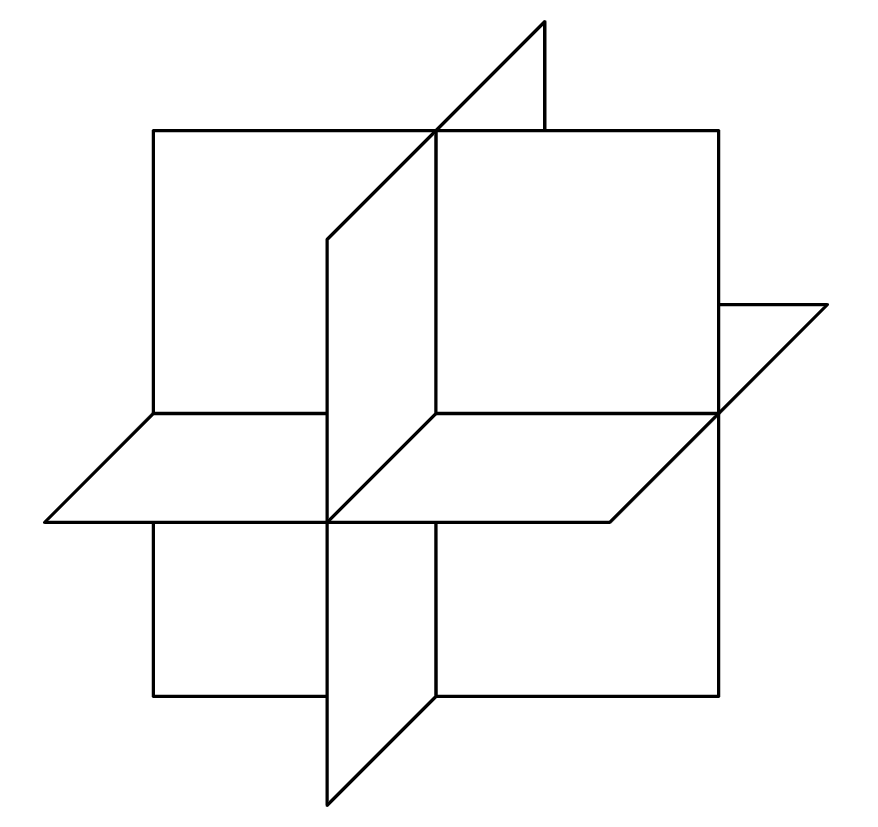
\includegraphics[width=\textwidth]{planeintersection1}} \\
& & & \\ \hline[1pt]
\SetCell[r=1,c=4]{c} $\det\boldsymbol{M}=0$ \\ \hline[1pt]
\SetCell[r=2,c=1]{c}2&\SetCell[r=2,c=1]{l}\begin{tabular}{l}Planes all parallel and \\none coincident\\\end{tabular} & \SetCell[r=8,c=1]{c}No solutions & \SetCell[r=2,c=1]{c}\scalebox{.25}{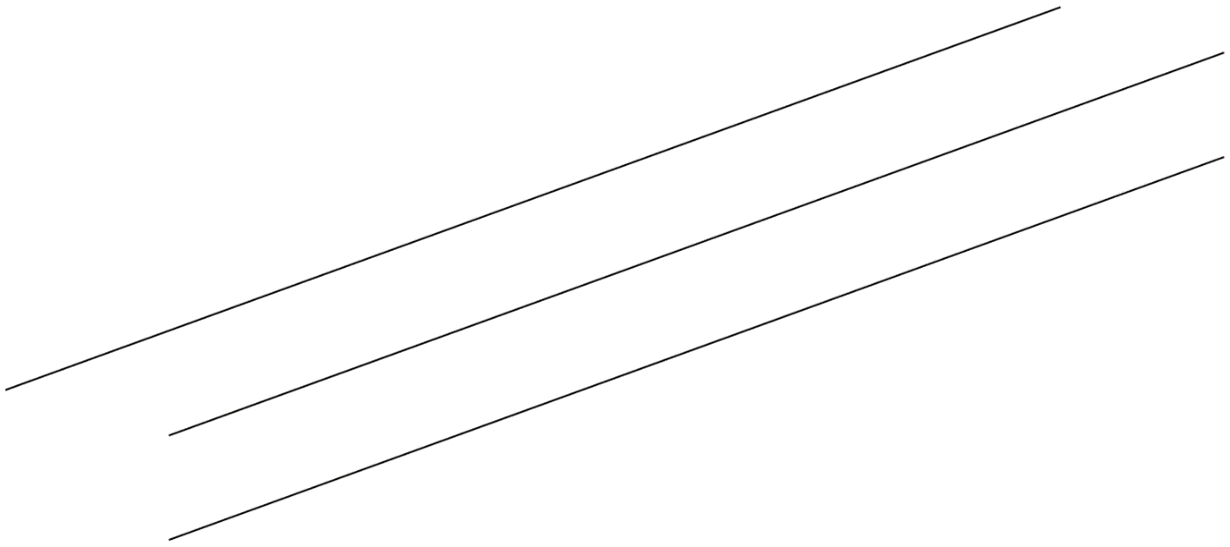
\includegraphics[width=\textwidth]{planeintersection21}} \\
& & & \\ \hline
\SetCell[r=2,c=1]{c}3&\SetCell[r=2,c=1]{l}\begin{tabular}{l}Planes all parallel and \\ only two coincident\end{tabular} &  & \SetCell[r=2,c=1]{c}\scalebox{.25}{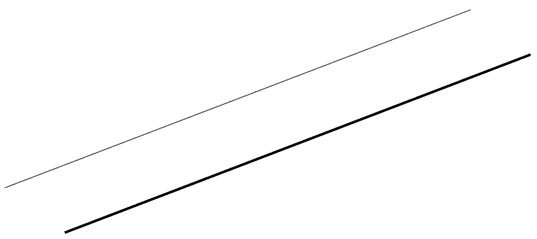
\includegraphics[width=\textwidth]{planeintersection31}} \\
& & & \\ \hline
\SetCell[r=2,c=1]{c}4&\SetCell[r=2,c=1]{l}\begin{tabular}{l}Two planes parallel but \\ non-coincident, with \\one traversing\end{tabular} &  & \SetCell[r=2,c=1]{c}\scalebox{.25}{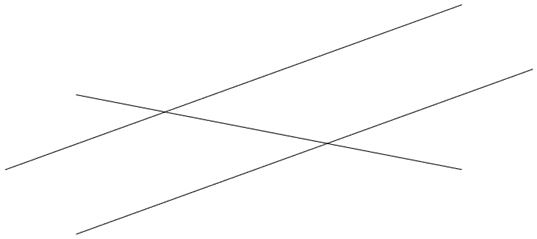
\includegraphics[width=\textwidth]{planeintersection41}} \\
& & & \\ \hline
\SetCell[r=2,c=1]{c}5&\SetCell[r=2,c=1]{l}\begin{tabular}{l}Planes intersect to form \\a triangular prism\end{tabular} &  & \SetCell[r=2,c=1]{c}\scalebox{.25}{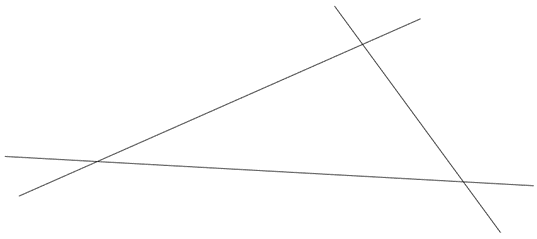
\includegraphics[width=\textwidth]{planeintersection51}} \\
& & & \\ \hline[1pt]
\SetCell[r=2,c=1]{c}6&\SetCell[r=2,c=1]{l}\begin{tabular}{l}Planes form a sheaf\end{tabular} & \SetCell[r=4,c=1]{c}Line of solutions & \SetCell[r=2,c=1]{c}\scalebox{.25}{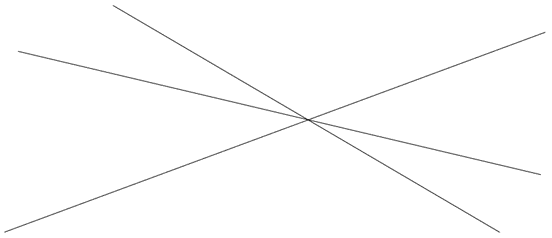
\includegraphics[width=\textwidth]{planeintersection61}} \\
& & & \\ \hline
\SetCell[r=2,c=1]{c}7&\SetCell[r=2,c=1]{l}\begin{tabular}{l}Two planes coincident \\with one traversing\end{tabular} &  & \SetCell[r=2,c=1]{c}\scalebox{.25}{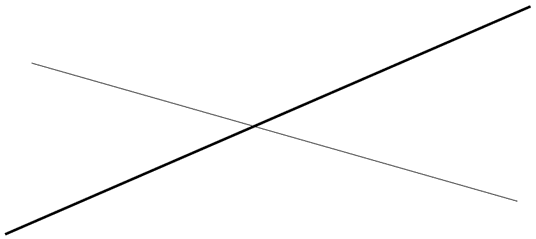
\includegraphics[width=\textwidth]{planeintersection71}} \\
& & & \\ \hline[1pt]
\SetCell[r=2,c=1]{c}8&\SetCell[r=2,c=1]{l}\begin{tabular}{l}Three planes coincident\end{tabular} & \SetCell[r=2,c=1]{c}Plane of solutions & \SetCell[r=2,c=1]{c}\scalebox{.25}{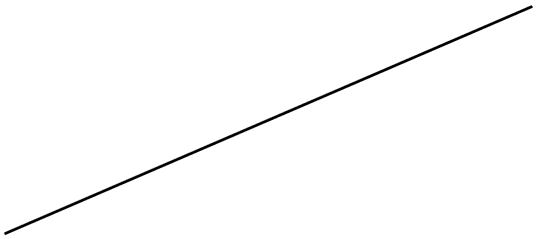
\includegraphics[width=\textwidth]{planeintersection81}} \\ 
& & & \\ \hline[1pt]
\end{tblr}
\end{center}
\normalsize
\vspace{0.5cm}

\newpage
\subsection{Examples of configurations of three planes in three dimensions}
\label{planesexamples}
\begin{itemize}
\item A Level FM Year 2 \hspace{1cm} \phantom{AS /} Pages 104 -- 110
\end{itemize} \par
\begin{center}
\scriptsize
\begin{tblr}{|[1pt]|c|c|c|c||[1pt]}
\hline[1pt]
\# & System & Matrix equation & Nature of solution\\ \hline[1pt]
\SetCell[r=1,c=4]{c} $\det\boldsymbol{M}\neq0$ \\ \hline[1pt]
\SetCell[r=2,c=1]{c}1&\SetCell[r=2,c=1]{c} \parbox{1cm}{\vspace{-.4cm}\begin{align*}
4x-\phantom{3}y-\phantom{4}z&=17\\
x+\phantom{3}y-4z&=3\\
2x-3y+2z&=6 
\end{align*}\vspace{-.4cm}}& \SetCell[r=2,c=1]{c} $\begin{bmatrix}4&-1&-1\\1&\phantom{-}1&-4\\2&-3&\phantom{-}2\end{bmatrix}\begin{bmatrix}x\\y\\z\end{bmatrix}=\begin{bmatrix}17\\3\\6\end{bmatrix}$ & \SetCell[r=2,c=1]{c} \parbox{3cm}{\vspace{-.4cm}Planes intersect at a single point\vspace{-.4cm}} \\
& & & \\ \hline[1pt]
\SetCell[r=1,c=4]{c} $\det\boldsymbol{M}=0$ \\ \hline[1pt]
\SetCell[r=2,c=1]{c}2&\SetCell[r=2,c=1]{c}\parbox{1cm}{\vspace{-.4cm}\begin{align*}
2x-2y+4z&=20\\
3x-3y+6z&=24\\
x-\phantom{3}y+2z&=5 
\end{align*}\vspace{-.4cm}} & \SetCell[r=2,c=1]{c} $\begin{bmatrix}2&-2&\phantom{-}4\\3&-3&\phantom{-}6\\1&-1&\phantom{-}2\end{bmatrix}\begin{bmatrix}x\\y\\z\end{bmatrix}=\begin{bmatrix}20\\24\\5\end{bmatrix}$ & \SetCell[r=2,c=1]{c} \parbox{3cm}{\vspace{-.4cm}Planes all parallel and none coincident\vspace{-.4cm}} \\
& & & \\ \hline
\SetCell[r=2,c=1]{c}3&\SetCell[r=2,c=1]{c}\parbox{1cm}{\vspace{-.4cm}\begin{align*}
2x-2y+4z&=20\\
3x-3y+6z&=15\\
x-\phantom{3}y+2z&=5 
\end{align*}\vspace{-.4cm}}& \SetCell[r=2,c=1]{c} $\begin{bmatrix}2&-2&\phantom{-}4\\3&-3&\phantom{-}6\\1&-1&\phantom{-}2\end{bmatrix}\begin{bmatrix}x\\y\\z\end{bmatrix}=\begin{bmatrix}20\\15\\5\end{bmatrix}$ & \SetCell[r=2,c=1]{c} \parbox{3cm}{\vspace{-.4cm}Planes all parallel and only two coincident\vspace{-.4cm}} \\
& & & \\ \hline
\SetCell[r=2,c=1]{c}4&\SetCell[r=2,c=1]{c} \parbox{1cm}{\vspace{-.4cm}\begin{align*}
2x-2y+4z&=20\\
3x-3y+6z&=15\\
2x-3y+2z&=6 
\end{align*}\vspace{-.4cm}}& \SetCell[r=2,c=1]{c} $\begin{bmatrix}2&-2&\phantom{-}4\\3&-3&\phantom{-}6\\2&-3&\phantom{-}2\end{bmatrix}\begin{bmatrix}x\\y\\z\end{bmatrix}=\begin{bmatrix}20\\15\\6\end{bmatrix}$ & \SetCell[r=2,c=1]{c} \parbox{3cm}{\vspace{-.4cm}Two planes parallel but non-coincident, with one traversing\vspace{-.4cm}} \\
& & & \\ \hline
\SetCell[r=2,c=1]{c}5&\SetCell[r=2,c=1]{c} \parbox{1cm}{\vspace{-.4cm}\begin{align*}
4x-y-\phantom{4}z&=17\\
x+y-4z&=3\\
x-y+2z&=11
\end{align*}\vspace{-.4cm}}& \SetCell[r=2,c=1]{c} $\begin{bmatrix}4&-1&-1\\1&\phantom{-}1&-4\\1&-1&\phantom{-}2\end{bmatrix}\begin{bmatrix}x\\y\\z\end{bmatrix}=\begin{bmatrix}17\\3\\11\end{bmatrix}$ & \SetCell[r=2,c=1]{c} \parbox{3cm}{\vspace{-.4cm}Planes intersect to form a triangular prism\vspace{-.4cm}} \\
& & & \\ \hline[1pt]
\SetCell[r=2,c=1]{c}6&\SetCell[r=2,c=1]{c} \parbox{1cm}{\vspace{-.4cm}\begin{align*}
4x-y-\phantom{4}z&=17\\
x+y-4z&=3\\
x-y+2z&=5 
\end{align*}\vspace{-.4cm}}& \SetCell[r=2,c=1]{c} $\begin{bmatrix}4&-1&-1\\1&\phantom{-}1&-4\\1&-1&\phantom{-}2\end{bmatrix}\begin{bmatrix}x\\y\\z\end{bmatrix}=\begin{bmatrix}17\\3\\5\end{bmatrix}$ & \SetCell[r=2,c=1]{c} \parbox{3cm}{\vspace{-.4cm}Planes form a sheaf\vspace{-.4cm}} \\
& & & \\ \hline
\SetCell[r=2,c=1]{c}7&\SetCell[r=2,c=1]{c} \parbox{1cm}{\vspace{-.4cm}\begin{align*}
2x-2y+4z&=10\\
3x-3y+6z&=15\\
2x-3y+2z&=6 
\end{align*}\vspace{-.4cm}}& \SetCell[r=2,c=1]{c} $\begin{bmatrix}2&-2&\phantom{-}4\\3&-3&\phantom{-}6\\2&-3&\phantom{-}2\end{bmatrix}\begin{bmatrix}x\\y\\z\end{bmatrix}=\begin{bmatrix}10\\15\\6\end{bmatrix}$ & \SetCell[r=2,c=1]{c} \parbox{3cm}{\vspace{-.4cm}Two planes coincident with one traversing\vspace{-.4cm}} \\
& & & \\ \hline[1pt]
\SetCell[r=2,c=1]{c}8&\SetCell[r=2,c=1]{c} \parbox{1cm}{\vspace{-.4cm}\begin{align*}
2x-2y+4z&=10\\
3x-3y+6z&=15\\
x-\phantom{3}y+2z&=5 
\end{align*}\vspace{-.4cm}}& \SetCell[r=2,c=1]{c} $\begin{bmatrix}2&-2&\phantom{-}4\\3&-3&\phantom{-}6\\1&-1&\phantom{-}2\end{bmatrix}\begin{bmatrix}x\\y\\z\end{bmatrix}=\begin{bmatrix}10\\15\\5\end{bmatrix}$ & \SetCell[r=2,c=1]{c} \parbox{3cm}{\vspace{-.4cm}Three planes coincident\vspace{-.4cm}} \\
& & & \\ \hline[1pt]
\end{tblr}
\end{center}
\vspace{0.25cm}

\newpage
\subsection{Linear transformations - matrices}
\begin{itemize}
\item A Level FM AS / Year 1 \hspace{1cm} Pages 1 -- 7
\item A Level FM AS / Year 1 \hspace{1cm} Pages 71 -- 94
\item A Level FM Year 2 \hspace{1cm} \phantom{AS /} Pages 101 -- 104
\end{itemize} \par

Linear transformations map points from one to another, and can be represented by matrices.
\begin{equation*}
\begin{bmatrix} a & b \\ c& d\end{bmatrix}\begin{bmatrix} x \\ y \end{bmatrix}=\begin{bmatrix} ax+by \\ cx+dy\end{bmatrix}
\end{equation*}
\begin{itemize}
\item[-]Linear transformations maintain parallel lines, though perpendicular lines may not always be maintained.
\item[-]The origin $(0,0)$ is \emph{always} mapped onto itself by a linear transformation.
	\item[-]Using matrix $\boldsymbol{A}$ and then $\boldsymbol{B}$, where $\boldsymbol{A}=\begin{bmatrix} a & b \\ c& d\end{bmatrix}$, and $\boldsymbol{B}=\begin{bmatrix} p & q \\ r & s \end{bmatrix}$, on $\begin{bmatrix} x \\ y \end{bmatrix}$ is represented as $\boldsymbol{BA}\begin{bmatrix} x\\ y\end{bmatrix}$, and the matrix $\boldsymbol{BA}$ is
\begin{equation*}
\boldsymbol{BA}=\begin{bmatrix} p & q \\ r& s\end{bmatrix}\begin{bmatrix} a & b \\ c& d\end{bmatrix}=\begin{bmatrix} pa+qc & pb+qd \\ ra+sc& rb+sd\end{bmatrix}
\end{equation*}
\item[-]The identity matrix is 
\begin{equation*}
\begin{bmatrix} 1 & 0 \\ 0& 1\end{bmatrix}
\end{equation*}
and maps every point to itself. Its algebraic equivalent is multiplying by 1.
The first column of a matrix is where the vector $\hat{\boldsymbol{\imath}}$ maps to. The second column is where the vector $\hat{\boldsymbol{\jmath}}$ maps to. For a three-dimensional matrix, the third column is where the vector $\hat{\boldsymbol{k}}$ maps to.
\item[-]A $2\times2$ anticlockwise rotation matrix of an angle $\theta$ has the form
\begin{equation*}
\begin{bmatrix} \cos(\theta) & -\sin(\theta) \\ \sin(\theta) & \cos(\theta) \end{bmatrix}
\end{equation*}
\item[-] Linear transformations include \emph{reflections}, \emph{rotations}, \emph{enlargements}, and \emph{shears}, or can be a combination of any of them
\item[-] \textbf{\underline{Invariant lines}} are lines which do not move under the transformation
\item[-] \textbf{\underline{Invariant points}} are points which do not move under the transformation
\end{itemize} \par
\vspace{0.5cm}

\subsection{Standard matrices}
\begin{itemize}
\item A Level FM AS / Year 1 \hspace{1cm} Pages 81 -- 82
\item A Level FM AS / Year 1 \hspace{1cm} Pages 90 -- 91
\end{itemize} \par
The $2\times2$ matrices you should recognise are listed below.
\scriptsize
\begin{center}
\begin{tblr}{|[.75pt]|l|cc|c||[.75pt]}
\hline[1pt]
Transformation & \SetCell[r=1,c=2]{c} Matrix & &Determinant \\ \hline[.75pt]
\SetCell[r=2,c=1]{l} \parbox{3cm}{Anticlockwise rotation about $O$, angle $\theta$} & \SetCell[r=2,c=2]{c}$\begin{bmatrix}\cos(\theta) & -\sin(\theta) \\ \sin(\theta)&\cos(\theta)\end{bmatrix}$ & &\SetCell[r=2,c=1]{c}1 \\
& & & \\ \hline
\SetCell[r=2,c=1]{l} \parbox{3cm}{Reflection in coordinate axes} & \SetCell[r=2,c=1]{c}\parbox{1.5cm}{\vspace{-.5cm}\begin{gather*}x\text{-axis} \\ \begin{bmatrix}1 & 0 \\ 0&-1\end{bmatrix}\end{gather*}\vspace{-.4cm}}& \SetCell[r=2,c=1]{c}\parbox{1.5cm}{\vspace{-.5cm}\begin{gather*}y\text{-axis} \\ \begin{bmatrix}-1 & 0 \\ 0&1\end{bmatrix}\end{gather*}\vspace{-.4cm}} & \SetCell[r=2,c=1]{c}-1 \\
& & & \\ \hline
\SetCell[r=2,c=1]{l} \parbox{3cm}{Reflection in the lines $y=\pm x$} & \SetCell[r=2,c=2]{c}$\begin{bmatrix}0 & \pm1 \\ \pm1&0\end{bmatrix}$ & &\SetCell[r=2,c=1]{c}-1 \\
& & & \\ \hline
\SetCell[r=2,c=1]{l} \parbox{3cm}{Stretch, scale factor $c$, with the $y$-axis invariant} & \SetCell[r=2,c=2]{c}$\begin{bmatrix}c & 0 \\ 0&1\end{bmatrix}$ & &\SetCell[r=2,c=1]{c}$c$ \\
& & & \\ \hline
\SetCell[r=2,c=1]{l} \parbox{3cm}{Stretch, scale factor $d$, with the $x$-axis invariant} & \SetCell[r=2,c=2]{c}$\begin{bmatrix}1 & 0 \\ 0&d\end{bmatrix}$ & &\SetCell[r=2,c=1]{c}$d$ \\
& & & \\ \hline
\SetCell[r=2,c=1]{l} \parbox{3cm}{Enlargement, centre $O$, scale factor $k$} & \SetCell[r=2,c=2]{c}$\begin{bmatrix}k & 0 \\ 0&k\end{bmatrix}$ & &\SetCell[r=2,c=1]{c}$k^{2}$ \\
& & & \\ \hline
\SetCell[r=2,c=1]{l} \parbox{3cm}{Shear, $x$-axis invariant,\\$(0,1)\rightarrow(k,1)$} & \SetCell[r=2,c=2]{c}$\begin{bmatrix}1 & k \\ 0&1\end{bmatrix}$ & &\SetCell[r=2,c=1]{c}1 \\
& & & \\ \hline
\SetCell[r=2,c=1]{l} \parbox{3cm}{Shear, $y$-axis invariant,\\$(1,0)\rightarrow(1,k)$} & \SetCell[r=2,c=2]{c}$\begin{bmatrix}1 & 0 \\ k&1\end{bmatrix}$ & &\SetCell[r=2,c=1]{c}1 \\
& & & \\ \hline[.75pt]
\end{tblr}
\end{center}
\normalsize
\par The $3\times3$ matrices you should recognise are reflections along the $x$-$y$, $x$-$z$, and $y$-$z$ planes, and rotations about each axis. Here are the anticlockwise rotations, followed by the reflections.
\begin{center}
\begin{tblr}{|[.75pt]|c|c|c||[.75pt]}
\hline[1pt]
$y$-$z$ plane ($x=0$) & $x$-$z$ plane ($y=0$) & $x$-$y$ plane ($z=0$) \\ \hline[.75pt]
$\begin{bmatrix} -1 & 0 & 0 \\ 0 & 1 & 0 \\ 0 & 0 & 1 \end{bmatrix}$ &
$\begin{bmatrix} 1 & 0 & 0 \\ 0 & -1 & 0 \\ 0 & 0 & 1 \end{bmatrix}$ &
$\begin{bmatrix} 1 & 0 & 0 \\ 0 & 1 & 0 \\ 0 & 0 & -1 \end{bmatrix}$ \\ \hline[.75pt]
\end{tblr}
\end{center}
\begin{center}
\begin{tblr}{|[.75pt]|c|c|c||[.75pt]}
\hline[1pt]
$x$-axis & $y$-axis & $z$-axis \\ \hline[.75pt]
$\begin{bmatrix} 1 & 0 & 0 \\ 0 & \cos(\theta) & -\sin(\theta) \\ 0 & \sin(\theta) & \cos(\theta) \end{bmatrix}$ &
$\begin{bmatrix} \cos(\theta) & 0 & \sin(\theta) \\ 0 & 1 & 0 \\ -\sin(\theta) & 0 & \cos(\theta) \end{bmatrix}$ &
$\begin{bmatrix} \cos(\theta) & -\sin(\theta) & 0 \\ \sin(\theta) & \cos(\theta) & 0 \\ 0 & 0 & 1 \end{bmatrix}$ \\ \hline[.75pt]
\end{tblr}
\end{center}
\vspace{0.5cm}

\newpage

\subsection{Matrix multiplication}
\begin{itemize}
\item A Level FM AS / Year 1 \hspace{1cm} Pages 7 -- 13
\end{itemize} \par
To multiply two matrices together, multiply the rows of the first matrix by columns of a second matrix. Two matrices can be multiplied if the number of columns in matrix $\boldsymbol{A}$ is equal to the number of rows in matrix $\boldsymbol{B}$. So if a $m\times n$ matrix multiplies an $n\times p$ matrix, the result is a $m\times p$ matrix.
\begin{equation*}
\begin{bmatrix}\cdot&\cdot&\cdot\\\cdot&\cdot&\cdot\\\cdot&\cdot&\cdot\\\cdot&\cdot&\cdot\end{bmatrix}\times\begin{bmatrix}\cdot&\cdot&\cdot&\cdot&\cdot\\\cdot&\cdot&\cdot&\cdot&\cdot\\\cdot&\cdot&\cdot&\cdot&\cdot\end{bmatrix}=\begin{bmatrix}\cdot&\cdot&\cdot&\cdot&\cdot\\\cdot&\cdot&\cdot&\cdot&\cdot\\\cdot&\cdot&\cdot&\cdot&\cdot\\\cdot&\cdot&\cdot&\cdot&\cdot\end{bmatrix}
\end{equation*}
\vspace{0.5cm}


\subsection{Determinant of a 2$\,\times\,$2 matrix}
\begin{itemize}
\item A Level FM AS / Year 1 \hspace{1cm} Pages 13 -- 23
\end{itemize} \par
For a matrix $\boldsymbol{M}=\begin{bmatrix}a&b\\c&d\end{bmatrix}$, the determinant is defined by
\begin{equation*}
\det \boldsymbol{M}=\det\begin{bmatrix}a&b\\c&d\end{bmatrix}=ad-bc
\end{equation*}
The determinant gives an area\footnote{volume in the case of a $3\times3$ matrix} scale factor of the matrix. \newline\par
If the determinant is negative, then it implies an inversion of the points (if points are $ABCD$ clockwise originally, then after matrix transformation, they will read $ADCB$ clockwise) \newline\par
If the determinant is $0$, then the matrix collapses space onto a line, or a point if $\boldsymbol{M}=\begin{bmatrix}0&0\\0&0\end{bmatrix}$
\begin{itemize}
\item[Note:] \begin{equation*}
\det \boldsymbol{MN}=\det \boldsymbol{M}\times\det \boldsymbol{N}
\end{equation*}
\end{itemize}
\vspace{0.5cm}

\newpage
\subsection{Inverse of a 2$\,\times\,$2 matrix}
\label{2x2inverse}
\begin{itemize}
\item A Level FM AS / Year 1 \hspace{1cm} Pages 13 -- 23
\end{itemize} \par
The inverse of a matrix $\boldsymbol{M}=\begin{bmatrix}a&b\\c&d\end{bmatrix}$ is defined by 
\begin{equation*}
\boldsymbol{M}^{-1}=\frac{1}{\det \boldsymbol{M}}\begin{bmatrix}d&-b\\-c&a\end{bmatrix}=\begin{bmatrix}\frac{d}{ad-bc}&\frac{-b}{ad-bc}\\\frac{-c}{ad-bc}&\frac{a}{ad-bc}\end{bmatrix}
\end{equation*} \newline \par
We can use the inverse of a matrix to solve a pair of simultaneous equations. Given the equations
\begin{equation*}
\begin{Bmatrix}2x+y=4 \\ 3x+4y=11 \end{Bmatrix}
\end{equation*}
These can be represented by the matrix equation
\begin{equation*}
\begin{bmatrix}2&1\\3&4\end{bmatrix}\begin{bmatrix}x\\y\end{bmatrix}=\begin{bmatrix}4\\11\end{bmatrix}
\end{equation*}
So, by taking the inverse matrix and applying it to both sides,
\begin{align*}
\begin{bmatrix}x\\y\end{bmatrix}&=\frac{1}{2\times4-3\times1}\begin{bmatrix}4&-1\\-3&2\end{bmatrix}\begin{bmatrix}4\\11\end{bmatrix} \\
\begin{bmatrix}x\\y\end{bmatrix}&=\frac{1}{5}\begin{bmatrix} 4\times4-1\times11 \\ -3\times4+2\times11 \end{bmatrix}\\
\begin{bmatrix}x\\y\end{bmatrix}&=\frac{1}{5}\begin{bmatrix} 5 \\ 10 \end{bmatrix}\\
\begin{bmatrix}x\\y\end{bmatrix}&=\begin{bmatrix}1\\2\end{bmatrix}\\
\end{align*}
In the case that the determinant of the matrix is zero, then no unique solutions to the system exists.
\vspace{0.5cm}


\subsection{Determinant of a 3$\,\times\,$3 matrix}
\begin{itemize}
\item A Level FM AS / Year 1 \hspace{1cm} Pages 23 -- 29
\end{itemize} \par
In the same way that the determinat of a $2\times2$ matrix is the signed scale factor of the transformed unit square defined by $\hat{\boldsymbol{\imath}}$ and $\hat{\boldsymbol{\jmath}}$, the determinant of a $3\times3$ matrix is the signed volume scale factor of the transformed unit cube defined by $\hat{\boldsymbol{\imath}}$, $\hat{\boldsymbol{\jmath}}$ and $\hat{\boldsymbol{k}}$. \newline \par

Therefore if $\boldsymbol{M}=\begin{bmatrix} \uparrow & \uparrow & \uparrow \\ \boldsymbol{a} & \boldsymbol{b} & \boldsymbol{c} \\ \downarrow & \downarrow & \downarrow \end{bmatrix}$, then 
\begin{equation*}
\det\boldsymbol{M}=\boldsymbol{a}\cdot(\boldsymbol{b}\times\boldsymbol{c})=\boldsymbol{b}\cdot(\boldsymbol{c}\times\boldsymbol{a})=\boldsymbol{c}\cdot(\boldsymbol{a}\times\boldsymbol{b})
\end{equation*} (Treat the first column as a vector $\boldsymbol{a}$, the second as a vector $\boldsymbol{b}$, and the third as a vector $\boldsymbol{c}$)\newline \par

There are three cases for the determinant:
\begin{itemize}
\item[-]$\det\boldsymbol{M}>0 \hspace{.5cm}$ the transformation preserves the order of the axes (e.g. a rotation)
\item[-]$\det\boldsymbol{M}<0 \hspace{.5cm}$ the transformation reverses the order of the axes (e.g. a reflection)
\item[-]$\det\boldsymbol{M}=0 \hspace{.5cm}$ the transformation maps three dimensional space to a plane, a point, or a line.
\end{itemize}
\vspace{0.5cm}


\subsection{Inverse of a 3$\,\times\,$3 matrix}
\begin{itemize}
\item A Level FM AS / Year 1 \hspace{1cm} Pages 23 -- 29
\end{itemize} \par
For $\boldsymbol{M}=\begin{bmatrix} \uparrow & \uparrow & \uparrow \\ \boldsymbol{a} & \boldsymbol{b} & \boldsymbol{c} \\ \downarrow & \downarrow & \downarrow \end{bmatrix}=\begin{bmatrix}a_{1}&b_{1}&c_{1}\\a_{2}&b_{2}&c_{2}\\a_{3}&b_{3}&c_{3}\\ \end{bmatrix}$ and $\begin{bmatrix} \leftarrow & \boldsymbol{p} & \rightarrow \\ \leftarrow & \boldsymbol{q} & \rightarrow \\ \leftarrow & \boldsymbol{r} & \rightarrow \end{bmatrix}=\begin{bmatrix}p_{1}&p_{2}&p_{3}\\q_{1}&q_{2}&q_{3}\\r_{1}&r_{2}&r_{3}\\\end{bmatrix}$
\begin{equation*}
\begin{bmatrix} \leftarrow & \boldsymbol{p} & \rightarrow \\ \leftarrow & \boldsymbol{q} & \rightarrow \\ \leftarrow & \boldsymbol{r} & \rightarrow \end{bmatrix}\begin{bmatrix} \uparrow & \uparrow & \uparrow \\ \boldsymbol{a} & \boldsymbol{b} & \boldsymbol{c} \\ \downarrow & \downarrow & \downarrow \end{bmatrix}=\begin{bmatrix} \boldsymbol{p}\cdot\boldsymbol{a} & \boldsymbol{p}\cdot\boldsymbol{b} & \boldsymbol{p}\cdot\boldsymbol{c} \\ \boldsymbol{q}\cdot\boldsymbol{a} & \boldsymbol{q}\cdot\boldsymbol{b} & \boldsymbol{q}\cdot\boldsymbol{c} \\ \boldsymbol{r}\cdot\boldsymbol{a} & \boldsymbol{r}\cdot\boldsymbol{b} & \boldsymbol{r}\cdot\boldsymbol{c} \end{bmatrix}
\end{equation*}
And we want something of the form
\begin{equation*}
\begin{bmatrix} \leftarrow & \boldsymbol{p} & \rightarrow \\ \leftarrow & \boldsymbol{q} & \rightarrow \\ \leftarrow & \boldsymbol{r} & \rightarrow \end{bmatrix}\begin{bmatrix} \uparrow & \uparrow & \uparrow \\ \boldsymbol{a} & \boldsymbol{b} & \boldsymbol{c} \\ \downarrow & \downarrow & \downarrow \end{bmatrix}=\begin{bmatrix} ? & 0 & 0 \\ 0 & ? & 0 \\ 0 & 0 & ? \end{bmatrix}
\end{equation*}
Therefore, we need 
\begin{align*}
\boldsymbol{p}\cdot\boldsymbol{b}&=0 & \boldsymbol{p}\cdot\boldsymbol{c}&=0 & \text{Try }\boldsymbol{p}=\boldsymbol{b}\times\boldsymbol{c}\\
\boldsymbol{q}\cdot\boldsymbol{a}&=0 & \boldsymbol{q}\cdot\boldsymbol{c}&=0 & \text{Try }\boldsymbol{q}=\boldsymbol{c}\times\boldsymbol{a}\\
\boldsymbol{r}\cdot\boldsymbol{a}&=0 & \boldsymbol{r}\cdot\boldsymbol{b}&=0 & \text{Try }\boldsymbol{r}=\boldsymbol{a}\times\boldsymbol{b}
\end{align*}

Therefore
\begin{align*}
\begin{bmatrix} \leftarrow & \boldsymbol{b}\times\boldsymbol{c} & \rightarrow \\ \leftarrow & \boldsymbol{c}\times\boldsymbol{a} & \rightarrow \\ \leftarrow & \boldsymbol{a}\times\boldsymbol{b} & \rightarrow \end{bmatrix}\begin{bmatrix} \uparrow & \uparrow & \uparrow \\ \boldsymbol{a} & \boldsymbol{b} & \boldsymbol{c} \\ \downarrow & \downarrow & \downarrow \end{bmatrix}&=\begin{bmatrix} \boldsymbol{a}\cdot\boldsymbol{b}\times\boldsymbol{c} & 0 & 0 \\ 0 & \boldsymbol{b}\cdot\boldsymbol{c}\times\boldsymbol{a} & 0 \\ 0 & 0 & \boldsymbol{c}\cdot\boldsymbol{a}\times\boldsymbol{b} \end{bmatrix}\\
&=\det\boldsymbol{M}\begin{bmatrix}1&0&0\\0&1&0\\0&0&1\end{bmatrix}
\end{align*}

So
\begin{equation*}
\boldsymbol{M}^{-1}=\frac{1}{\det\boldsymbol{M}}\begin{bmatrix} \leftarrow & \boldsymbol{b}\times\boldsymbol{c} & \rightarrow \\ \leftarrow & \boldsymbol{c}\times\boldsymbol{a} & \rightarrow \\ \leftarrow & \boldsymbol{a}\times\boldsymbol{b} & \rightarrow \end{bmatrix}
\end{equation*} \newline \par

As in section \ref{2x2inverse}, we can solve a system of simultaneous equations in three variable by way of a $3\times3$ matrix. Whether or not a unique solution exists can very simply be determined by taking the determinant of the matrix that represents the system. If the determinant \emph{is} 0, then more work is required.

\vspace{0.5cm}


\clearpage
\section{Exponents, logarithms, hyperbolic functions}
\vspace{0.5cm}

\subsection{Laws of indices}
\begin{itemize}
\item A Level M AS / Year 1 \hspace{1cm} \phantom{ } Pages 17 -- 21
\end{itemize} \par
\begin{itemize}
\item[-] Given the expression:
\begin{equation*}
a^{n}
\end{equation*}
$a$ is the base, and $n$ is the index / exponent
\item[-]A negative index gives a reciprocal
\begin{equation*}
a^{-n}=\frac{1}{a^{n}}=\left(\frac{1}{a}\right)^{n}
\end{equation*}
\item[-] Fractions in the exponent correspond to surds / roots of the base
\begin{equation*}
x^{\frac{a}{b}}=\sqrt[b]{x^{a}}=\left(\sqrt[b]{x}\right)^{a}
\end{equation*}
\end{itemize}
\vspace{0.5cm}


\subsection{Laws of logarithms}
\begin{itemize}
\item A Level M AS / Year 1 \hspace{1cm} \phantom{ } Pages 114 -- 126
\end{itemize}
\begin{flalign*}
\log_{a}(x)&=b \text{ means } a^{b}=x & \log_{a}\left(x^{n}\right)&=n\log_{a}(x)&& \\
\log_{a}\left(a^{x}\right)&=x & \log_{a}(xy)&=\log_{a}(x)+\log_{a}(y) && \\
\log_{a}(1)&=0 & \log_{a}\left(\frac{x}{y}\right)&=\log_{a}(x)-\log_{a}(y) &&
\end{flalign*}
The last two rules, for $\log_{a}(xy)$ and $\log_{a}\left(\frac{x}{y}\right)$ can be proved fairly simply. The proof for $\log_{a}(xy)$ is detailed below, and the proof for $\log_{a}\left(\frac{x}{y}\right)$ follows a very similar method.
\begin{equation*}
xy=\left( a^{\log_{a}(x)} \right)\left( a^{\log_{a}(y)} \right) = a^{\log_{a}(x)+\log_{a}(y)} = a^{\log_{a}(xy)}
\end{equation*}

\newpage


\subsection{Euler's number, `$e$'}
\begin{itemize}
\item A Level M Year 2 \hspace{1cm} \phantom{ AS / } Pages 185 -- 195
\end{itemize} \par
The number $e$ is defined such that
\begin{equation*}
f(x)=f'(x)
\end{equation*}
This is called the exponential function;
\begin{equation*}
f(x)=e^{x}=\exp(x)
\end{equation*}

From first principles,
\begin{flalign*}
\frac{\mathrm{d}}{\mathrm{d}x}[f(x)]&=\lim_{h \to 0} \left[ \frac{f(x+h)-f(x)}{h} \right] && \\
&=\lim_{h \to 0} \left[ \frac{e^{x+h}-e^{x}}{h} \right] && \\
&=\lim_{h \to 0} \left[ \frac{e^{x}\left(e^{h}-1\right)}{h} \right] && \\
&=e^{x}\lim_{h \to 0} \left[ \frac{\left(e^{h}-1\right)}{h} \right] \hspace{1cm} \text{and }\lim_{h \to 0} \left[ \frac{\left(e^{h}-1\right)}{h} \right]=1&& \\
&=e^{x}\times 1 && \\
&=e^{x} \hspace{1cm} \text{ as required}
\end{flalign*}
The logarithm with base $e$ is commonly denoted as
\begin{equation*}
\log_{e}(x)=\ln(x)
\end{equation*}
and is called the \emph{natural logarithm}
\begin{itemize}
\item[Note:] The chain rule still applies when differentiating, therefore:
\begin{equation*}
\frac{\mathrm{d}}{\mathrm{d}x}\left[ e^{f(x)} \right] = e^{f(x)} \times \frac{\mathrm{d}}{\mathrm{d}x}\left[ f(x) \right]
\end{equation*}
\end{itemize}
\vspace{0.5cm}


\subsection{Exponential models}
\begin{itemize}
\item A Level M AS / Year 1 \hspace{1cm} \phantom{ } Pages 128 -- 145
\end{itemize} \par
Exponential models are characterised by the following properties;
\begin{itemize}
\item[-] Where $A$ and $b$ are constants;\begin{equation*}y=Ae^{bx}\end{equation*}
\item[-] Rate of change is proportional to the remaining / current quantity
\begin{equation*}\frac{\mathrm{d}y}{\mathrm{d}x}=b\cdot Ae^{bx}=b\cdot y \end{equation*}
\item[-] Fixed changes in the $x$ value correspond with fixed \emph{scale factor} changes in the output
\item[-]Exponential models can be linearised by taking natural logarithms of both sides
\begin{align*}
y&=Ae^{bx} \\
\ln(y)&=\ln\left(Ae^{bx}\right) \\
&=\ln(A)+\ln\left(e^{bx}\right) \\
&=\ln(A)+b\ln(e^{x}) \\
&=\ln(A)+bx
\end{align*}
\end{itemize}
\vspace{0.5cm}


\subsection{The derivative of ln(x)}
\begin{itemize}
\item A Level M Year 2 \hspace{1cm} \phantom{ AS / } Pages 214 -- 216
\end{itemize} \par
The derivative of $\ln(x)$ is
\begin{equation*}
\frac{\mathrm{d}}{\mathrm{d}x}\left[ \ln(x) \right]=\frac{1}{x}
\end{equation*}
and so the integral of $\frac{1}{x}$ is 
\begin{equation*}
\int\frac{1}{x}=\ln(x)+c
\end{equation*}
Again, this can be used in conjunction with the chain rule. A couple of examples follow:
\begin{align*}
\frac{\mathrm{d}}{\mathrm{d}x}\left[ \ln(something) \right]&=\frac{1}{(something)}\times\frac{\mathrm{d}}{\mathrm{d}x}\left[ something \right] \\
\frac{\mathrm{d}}{\mathrm{d}x}\left[ \ln\left(\sin(x)\right) \right]&=\frac{1}{\sin(x)}\times\cos(x)=\cot(x) \\
\frac{\mathrm{d}}{\mathrm{d}x}\left[ \sin\left(\ln(x)\right) \right]&=\cos\left(\ln(x)\right)\times\frac{1}{x}=\frac{\cos\left(\ln(x)\right)}{x} \\
\end{align*}


\subsection{Expanding the domain -- ln(|x|)}
The function $y=\ln(x)$ only is valid for inputs of $x>0$. However, the curve $y=\frac{1}{x}$ is valid for $x\in\mathbb{R}\setminus{0}$. Therefore to expand the validity of $ln(x)$ as a solution to the integral of $\frac{1}{x}$, we must use the modulus of $x$ inside the argument of the natural logarithm.
\begin{align*}
\frac{\mathrm{d}}{\mathrm{d}x}\left[ \ln(x) \right]&=\frac{1}{x} \, \, \text{for } x>0 \\
\frac{\mathrm{d}}{\mathrm{d}x}\left[ \ln\left(\textcolor{red}{|}x\textcolor{red}{|}\right) \right]&=\frac{1}{x} \, \, \text{for } x\in\mathbb{R}\setminus{0} \\
\end{align*}


\subsection{The hyperbolic functions}
\begin{itemize}
\item A Level FM Year 2 \hspace{1cm} \phantom{AS /} Pages 129 -- 131
\item A Level FM Year 2 \hspace{1cm} \phantom{AS /} Pages 138 -- 142
\end{itemize} \par
The \emph{hyperbolic} functions are defined as follows:
\begin{gather*}
\cosh(x)=\frac{e^{x}+e^{-x}}{2} \\
\sinh(x)=\frac{e^{x}-e^{-x}}{2} \\
\tanh(x)=\frac{\sinh(x)}{\cosh(x)}=\frac{e^{x}-e^{-x}}{e^{x}+e^{-x}}
\end{gather*}
Each with domain $\mathbb{R}$ \newline \par

The \emph{inverse hyperbolic} functions are defined as follows:
\begin{align*}
\sech(x)&=\frac{1}{\cosh(x)}=\frac{e^{x}+e^{-x}}{2} \\
\cosech(x)&=\frac{1}{\sinh(x)}=\frac{e^{x}-e^{-x}}{2} \\
\coth(x)&=\frac{\cosh(x)}{\sinh(x)}=\frac{e^{x}+e^{-x}}{e^{x}-e^{-x}}
\end{align*}
Each with domain $\mathbb{R}$
\vspace{0.5cm}

\newpage

\subsection{Calculus of the hyperbolic functions}
\begin{itemize}
\item A Level FM Year 2 \hspace{1cm} \phantom{AS /} Pages 142 -- 149
\end{itemize} \par
\begin{flalign*}
\frac{\mathrm{d}}{\mathrm{d}x}\left[ \cosh(x) \right] &= \frac{\mathrm{d}}{\mathrm{d}x}\left[ \frac{e^{x}}{2}+\frac{e^{-x}}{2} \right]=\frac{e^{x}}{2}-\frac{e^{-x}}{2}=\frac{1}{2}\left(e^{x}-e^{-x}\right)=\sinh(x) && \\
\frac{\mathrm{d}}{\mathrm{d}x}\left[ \sinh(x) \right] &= \frac{\mathrm{d}}{\mathrm{d}x}\left[ \frac{e^{x}}{2}-\frac{e^{-x}}{2} \right]=\frac{e^{x}}{2}+\frac{e^{-x}}{2}=\frac{1}{2}\left(e^{x}+e^{-x}\right)=\cosh(x) && \\
\frac{\mathrm{d}}{\mathrm{d}x}\left[ \tanh(x) \right] &=\frac{\mathrm{d}}{\mathrm{d}x}\left[ \frac{e^{x}-e^{-x}}{e^{x}-e^{-x}} \right] && \\
&=\frac{\left( e^{x}+e^{-x} \right)\left( e^{x}+e^{-x} \right)-\left( e^{x}-e^{-x} \right)\left( e^{x}+e^{-x} \right)}{\left( e^{x}+e^{-x} \right)^{2}} && \\
&=\frac{\left( e^{x}+e^{-x} \right)^{2}-\left( e^{x}-e^{-x} \right)^{2}}{\left( e^{x}+e^{-x} \right)^{2}} && \\
&=\frac{\cancel{e^{2x}}+\cancel{e^{-2x}}+2-\cancel{e^{2x}}-\cancel{e^{-2x}}+2}{\left( e^{x}+e^{-x} \right)^{2}} && \\
&=\left( \frac{4}{\left( e^{x}+e^{-x} \right)^{2}} \right) = \left( \frac{2}{e^{x}+e^{-x}} \right)^{2}=\sech^{2}(x)&& \\
\end{flalign*}


\subsection{The inverse hyperbolic functions}
\begin{itemize}
\item A Level FM Year 2 \hspace{1cm} \phantom{AS /} Pages 131 -- 135
\end{itemize} \par
The inverse hyperbolic functions can be found by defining $y$ equal to the inverse function, rearranging to give $x$ in terms of $y$, so that $x$ is equal to the original hyperbolic, and then using the explicit form in exponentials to rearrange for $y$ in terms of $x$. This is demonstrated for the three hyperbolic functions below. \newline \par

\subsubsection*{arcosh}
\vspace{-0.8cm}
\begin{flalign*}
y&=\arcosh(x) && \\
x&=\cosh(y) && \\
x&=\frac{e^{y}+e^{-y}}{2} && \\
2x&=e^{y}+e^{-y} && \\
2x\cdot e^{y}&=e^{2y}+1 && \\
0&=\left( e^{y} \right)^{2}-2x\cdot e^{y}+1 \hspace{1cm} \text{This is simply a quadratic in $e^{y}$} && \\
e^{y}&=\frac{2x\pm\sqrt{4x^{2}-4}}{2} && \\
e^{y}&=x\pm\sqrt{x^{2}-1} && \\
y&=\ln\left( x+\sqrt{x^{2}-1} \right)
\end{flalign*}
Choose positive as convention, though both solutions satisfy the equation \newline \par

\subsubsection*{arsinh}
\vspace{-0.8cm}
\begin{flalign*}
y&=\arsinh(x) && \\
x&=\sinh(y) && \\
x&=\frac{e^{y}-e^{-y}}{2} && \\
2x&=e^{y}-e^{-y} && \\
2x\cdot e^{y}&=e^{2y}-1 && \\
0&=\left( e^{y} \right)^{2}-2x\cdot e^{y}-1 \hspace{1cm} \text{This is simply a quadratic in $e^{y}$} && \\
e^{y}&=\frac{2x\pm\sqrt{4x^{2}+4}}{2} && \\
e^{y}&=x\pm\sqrt{x^{2}+1} && \\
e^{y}&=x\textcolor{red}{+}\sqrt{x^{2}+1} && \\
y&=\ln\left( x+\sqrt{x^{2}+1} \right)
\end{flalign*}
We reject the $x-\sqrt{x^{2}+1}$ root, because $e^{y}>0$ and since $x^{2}+1>x^{2}$, $\sqrt{x^{2}+1}>x$, so $x-\sqrt{x^{2}+1}<0$, and so is not a valid solution. \newline \par

\subsubsection*{artanh}
\vspace{-0.8cm}
\begin{flalign*}
y=\artanh(x)& && \\
x=\tanh(y)=\frac{\sinh(x)}{\cosh(x)}&=\frac{e^{y}-e^{-y}}{e^{y}+e^{-y}}=\frac{e^{2y}-1}{e^{2y}+1} && \\
\left( e^{2y}+1 \right)x&=xe^{2y}+x=e^{2y}-1 && \\
xe^{2y}-e^{2y}&=-x-1 && \\
e^{2y}(x-1)&=(-x-1) && \\
e^{2y}&=\frac{1+x}{1-x} && \\
y&=\frac{1}{2}\ln\left(\frac{1+x}{1-x}\right)
\end{flalign*}

\subsection{Hyperbolic identities}
\begin{itemize}
\item A Level FM Year 2 \hspace{1cm} \phantom{AS /} Pages 136 -- 141
\end{itemize} \par
There are many identities involving hyperbolic functions, all of which are similar to trigonometric identities. The relationship between hyperbolic and trigonometric identities is covered by Osborne's Rule (section \ref{osborne}), but for now, here are the important ones to learn.
\begin{align*}
\cosh(x)+\sinh(x)&= e^{x} & \cosh(x)-\sinh(x)&= e^{-x} \\
\cosh^{2}(x)-\sinh^{2}(x)&= 1 & 1-\tanh^{2}(x)&=\sech^{2}(x) \\
\coth^{2}(x)-1&=\cosech^{2}(x) & \cosh^{2}+\sinh^{2}(x)&=\cosh(2x) \\
2\cosh^{2}(x)+1&=\cosh(2x) & 1+2\sinh^{2}(x)&=\cosh(2x) \\
\frac{2\tanh(x)}{1+\tanh^{2}(x)}&=\tanh(2x) & 2\sinh(x)\cosh(x)&=\sinh(2x)
\end{align*}

\begin{align*}
\cosh(x+y)&=\cosh(x)\cosh(y)+\sinh(x)\sinh(y) \\
\cosh(x)+\cosh(y)&=2\cosh\left( \frac{x+y}{2} \right)\cosh\left( \frac{x-y}{2} \right) \\
\end{align*}


\subsection{Osborne's Rule}
\label{osborne}
Osborne's Rule is a way of taking trigonometric identities, and obtaining its equivalent hyperbolic identity. See here the similarities between some trigonometric and hyperbolic identities;
\begin{align*}
\cos^{2}(x)+\sin^{2}(x)&=1 & \cosh^{2}(x)-\sinh^{2}(x)&=1 \\
\cos^{2}(x)-\sin^{2}(x)&=\cos(2x) & \cosh^{2}(x)+\sinh^{2}(x)&=\cosh(2x) \\
2\sin(x)\cos(x)&=\sin(2x) & 2\sinh(x)\cosh(x)&=\sinh(2x)
\end{align*}
Osborne's Rule:
\begin{enumerate}
\item Take a trigonometric identity involving terms of sine and cosine \textbf{\underline{only}}
\item Replace any $\sin$ terms with $\sinh$, and any $\cos$ terms with $\cosh$
\item Change the sign in front of any terms involving $\sinh^{2}$
\end{enumerate}
\vspace{0.5cm}


\subsection{Derivatives of the inverse hyperbolic functions}
\begin{itemize}
\item A Level FM Year 2 \hspace{1cm} \phantom{AS /} Pages 155 -- 162
\end{itemize} \par
Derivatives of the inverse hyperbolic functions can be found using implicit differentiation (see section \ref{implicitdifferentiation}). This is the origin of some of the standard integrals listed in section \ref{usefulintegrals}

\subsubsection*{arcosh}
\vspace{-0.8cm}
\begin{flalign*}
y&=\arcosh(x) && \\
x&=\cosh(y) && \\
1&=\sinh(y)\frac{\mathrm{d}y}{\mathrm{d}x} && \\
\frac{\mathrm{d}y}{\mathrm{d}x}&=\frac{1}{\sinh(y)}=\frac{1}{\pm\sqrt{\cosh^{2}(y)-1}}=\frac{1}{\pm\sqrt{x^{2}-1}}
\end{flalign*}
\begin{equation*}
\frac{\mathrm{d}y}{\mathrm{d}x}\left[\arcosh(x)\right]=\frac{1}{\sqrt{x^{2}-1}}
\end{equation*}

\subsubsection*{arsinh}
\vspace{-0.8cm}
\begin{flalign*}
y&=\arsinh(x) && \\
x&=\sinh(y) && \\
1&=\cosh(y)\frac{\mathrm{d}y}{\mathrm{d}x} && \\
\frac{\mathrm{d}y}{\mathrm{d}x}&=\frac{1}{\cosh(y)}=\frac{1}{\pm\sqrt{\sinh^{2}(y)+1}}=\frac{1}{\pm\sqrt{x^{2}+1}}
\end{flalign*}
\begin{equation*}
\frac{\mathrm{d}y}{\mathrm{d}x}\left[\arsinh(x)\right]=\frac{1}{\sqrt{x^{2}+1}}
\end{equation*}

\subsubsection*{artanh}
\vspace{-0.8cm}
\begin{flalign*}
y&=\artanh(x) && \\
x&=\tanh(y) && \\
1&=\sech^{2}(y)\frac{\mathrm{d}y}{\mathrm{d}x} && \\
\frac{\mathrm{d}y}{\mathrm{d}x}&=\frac{1}{\sech^{2}(y)}=\frac{1}{1-\tanh^{2}(y)}=\frac{1}{1-x^{2}}
\end{flalign*}
\begin{equation*}
\frac{\mathrm{d}y}{\mathrm{d}x}\left[\artanh(x)\right]=\frac{1}{1-x^{2}}
\end{equation*}
\vspace{0.5cm}



\clearpage
\section{Complex numbers}
\vspace{0.5cm}

\subsection{Algebraic closure, introduction to $\mathbb{C}$}
\begin{itemize}
\item A Level FM AS / Year 1 \hspace{1cm} Pages 110 -- 119
\end{itemize} \par
The imaginary unit $i$ is defined to be the square root of $-1$. Any number can be expressed in the form $z=x+iy$, where $z\in\mathbb{C}$, and $x,y\in\mathbb{R}$. \newline \par
For a complex number $z=x+iy$, its complex conjugate is defined as $z^{*}=x-iy$. \newline \par
To rationalise a denominator and `remove' the imaginary part from it, multiply the numerator and denominator by the complex conjugate of the denominator. \newline \par
Powers of $i$ follow a pattern, which extends to negative powers as well.
\begin{align*}
i^{1}&=i & i^{2}&=-1 & i^{3}&=-i & i^{4}&=1
\end{align*}
\vspace{0.25cm}


\subsection{Quadratics with $\mathbb{C}$}
\begin{itemize}
\item A Level FM AS / Year 1 \hspace{1cm} Pages 141 -- 159
\end{itemize} \par
Recalling section \ref{fundtheory}, any polynomial can be decomposed into real linear and / or irreducible quadratic factors. These irreducible quadratics are determined by whether their discriminant $\left(b^{2}-4ac\right)$ is greater than, equal to, or less than $0$. If the discriminant is less than zero, no real factors of the quadratic exist, but it can be split into a complex conjugate pair of linear roots.
\vspace{0.5cm}


\subsection{Argand diagram, modulus and argument}
\begin{itemize}
\item A Level FM AS / Year 1 \hspace{1cm} Pages 119 -- 129
\item A Level FM AS / Year 1 \hspace{1cm} Pages 134 -- 138
\item A Level FM Year 2 \hspace{1cm} \phantom{AS /} Pages 45 -- 52
\end{itemize} \par
An Argand diagram is a way of representing complex numbers; The real part is on the $x$-axis, and imaginary part on the $y$-axis.
\begin{figure}[H]
\centering
\scalebox{.5}{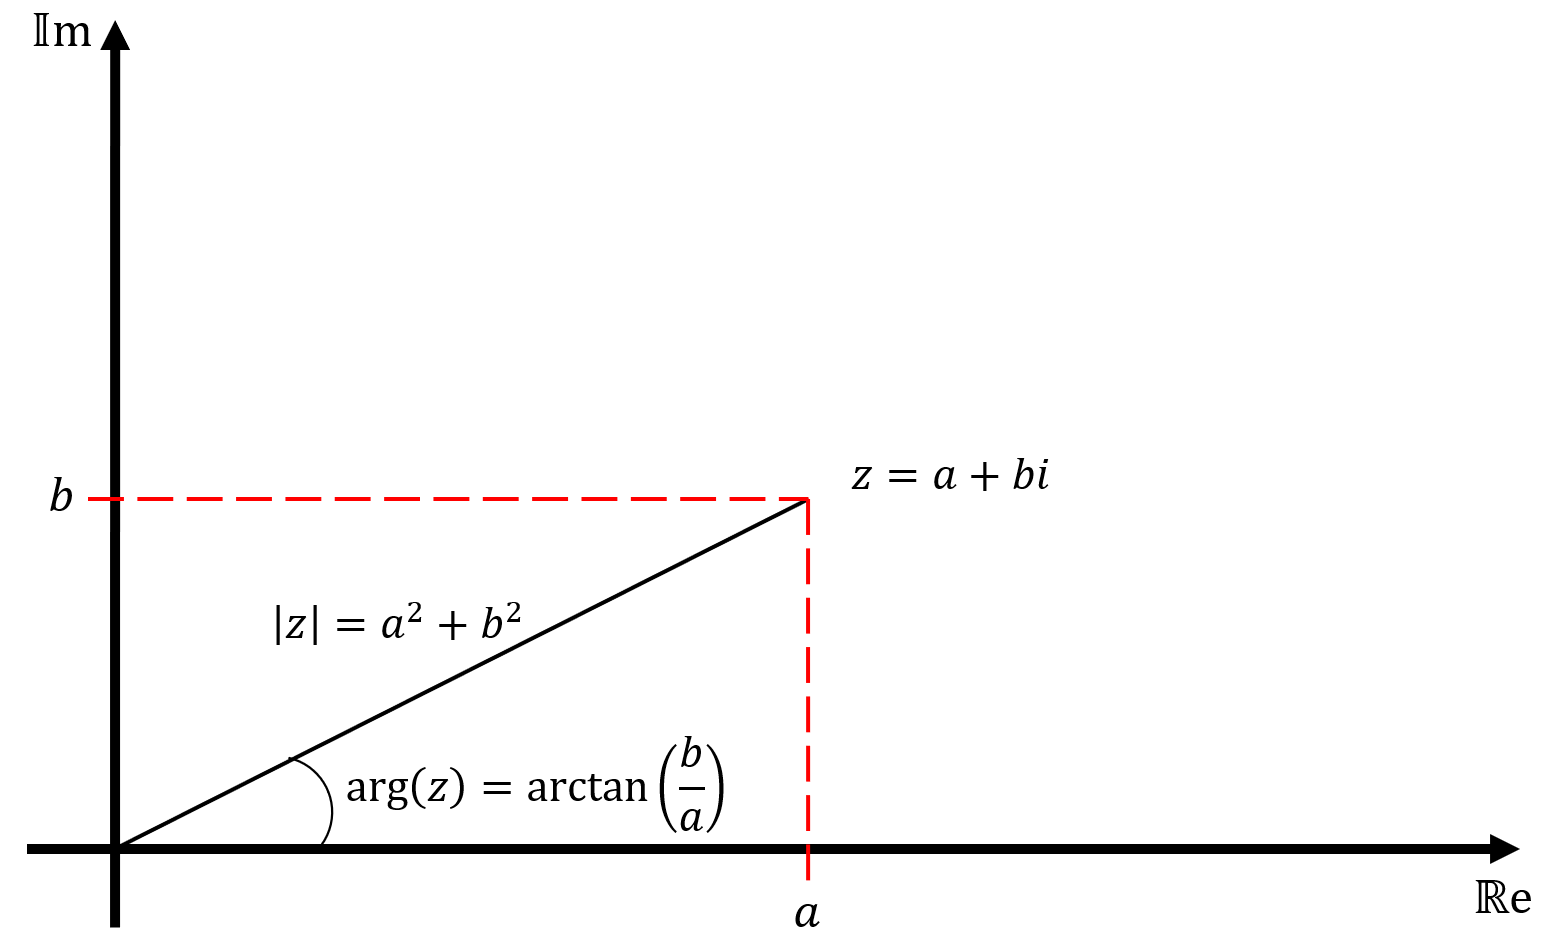
\includegraphics[width=\textwidth]{argand}}
\end{figure}
The modulus of a complex number $z=a+bi$ is given by the square root of $zz^{*}$, and is in effect the `length' of the vector that represents $z$ on an Argand diagram. The argument is the angle measured anticlockwise from the positive real axis. Of course, multiples of $2\pi$ can be added / subtracted to the argument, but the \underline{principle argument} is always in the interval $(-\pi,\pi)$.
\begin{align*}
z&=a+bi & z^{*}&=a-bi \\
\arg(z)&=\arctan\left(\frac{b}{a}\right) & \arg\left( z^{*} \right)&=\arctan\left(\frac{-b}{a}\right) \\
\end{align*}
\vspace{-1cm}
\begin{align*}
|z|&=\sqrt{zz^{*}}=\sqrt{(a+bi)(a-bi)}=\sqrt{a^{2}+\cancel{abi}-\cancel{abi}-(bi)^{2}} \\
&=\sqrt{a^{2}-b^{2}i^{2}}=\sqrt{a^{2}-b^{2}(-1)}=\sqrt{a^{2}+b^{2}}
\end{align*}

The complex number $z$ can therefore be written as
\begin{equation*}
z=r\left(\cos(\theta)+i\sin(\theta)\right)
\end{equation*}
where
\begin{align*}
r&=|z| & \theta&=\arg(z)
\end{align*}

When multiplying two complex numbers $w$ and $z$, the product, $wz$ can be evaluated fairly simply;
\begin{align*}
|wz|&=|w|\times|z| & \arg(wz)&=\arg(w)+\arg(z)
\end{align*}
\vspace{0.25cm}


\subsection{Complex number notation}
Where $z$ is a complex number with modulus $r$ and argument $\theta$;
\begin{center}
\small
\begin{tblr}{|[.75pt]|l|l||[.75pt]}
\hline[1pt]
Form & Name \\ \hline[1pt]
$z=x+iy$ & Cartesian form \\ \hline
$z=r\left(\cos(\theta)+i\sin(\theta)\right)\hspace{.5cm}$ & Modulus - argument form \\ \hline
$z=r \cis(\theta)$ & Polar form \\ \hline
$z=[r,\theta]$ & Polar form $\hspace{.5cm}$ \small{\emph{Note: Must be square brackets}} \\ \hline[.75pt]
\end{tblr}
\end{center}
\vspace{0.5cm}


\subsection{Loci in the complex plane}
\begin{itemize}
\item A Level FM AS / Year 1 \hspace{1cm} Pages 129 -- 134
\end{itemize} \par
As in section \ref{loci} on loci, a locus in the complex plane is a set of points which satisfy a certain condition. The formula booklet gives the following;
\begin{center}
\begin{tblr}{|[.75pt]|l|c||[.75pt]}
\hline[1pt]
Circles: & $|z-a|=k$ \\ \hline
Half lines: & $\arg(z-a)=\theta$ \\ \hline
Lines: & $|z-a|=|z-b|$ \\ \hline
\end{tblr}
\end{center}
Examples:
\begin{enumerate}
\item $|z-1-i|=1$
\begin{align*}
1&=\left|z-(1+i)\right| \\
1&=\left|x+iy-(1+i)\right|^{2} \\
1&=\left|(x-1)+i(y-1)\right|^{2} \\
1&=\left((x-1)+i(y-1)\right)\left((x-1)-i(y-1)\right) \\
1&=(x-1)^{2}+(y-1)^{2}
\end{align*}
\vspace{.3cm}
\item $\arg(z-2+i)=\frac{\pi}{4}$
\begin{equation*}
\arg\left(z-(2-i)\right)=\frac{\pi}{4}
\end{equation*}
The $z-(2-i)$ term maps the vector from (2-i) to $z$. This gives a half line, extending from the point representing $2-i$ in the direction with argument $\frac{\pi}{4}$
\vspace{.3cm}
\item $|z-(3+4i)|=|z-(2-5i)|$
\begin{align*}
\left|(x+iy)-(3+4i)\right|&=\left|(x+iy)-(2-5i)\right| \\
(x-3)^{2}+(y-4)^{2}&=(x-2)^{2}+(y+5)^{2} \\
\cancel{x^{2}}-6x+9 + \cancel{y^{2}}-8y+16 &= \cancel{x^{2}}-4x+4 + \cancel{y^{2}}+10y+25 \\
-2x-4&=18y \\
y&=\frac{-2x-4}{18}
\end{align*}
\end{enumerate}
\vspace{0.5cm}


\subsection{De Moivre's Theorem}
\begin{itemize}
\item A Level FM Year 2 \hspace{1cm} \phantom{AS /} Pages 25 -- 30
\item A Level FM Year 2 \hspace{1cm} \phantom{AS /} Pages 57 -- 64
\end{itemize} \par
De Moivre's Theorem states that:
\begin{equation*}
\left(\cos(\theta)+i\sin(\theta)\right)^{n}=\cos(n\theta)+i\sin(n\theta)
\end{equation*}
De Moivre's Theorem can be used to write $\cos(n\theta)$ or $\sin(n\theta)$ in terms of a sum of powers of $\cos(\theta)$ or $\sin(\theta)$ respectively.

Consider $\left(\\cos(\theta)+i\sin(\theta)\right)^{3}$. \newline \par
By De Moivre's Theorem;
\begin{equation*}
\left(\cos(\theta)+i\sin(\theta)\right)^{3}=\cos(3\theta)+i\sin(3\theta)
\end{equation*} \par
By expanding the binomial;
\scriptsize
\begin{align*}
\left(\cos(\theta)+i\sin(\theta)\right)^{3}&=\cos^{3}(\theta)+3i\cos^{2}(\theta)\sin(\theta)+3i^{2}\cos(\theta)\sin^{2}(\theta)+i^{3}\sin^{3}(\theta) \\
&=\cos^{3}(\theta)+3i\cos^{2}(\theta)\sin(\theta)-3\cos(\theta)\sin^{2}(\theta)-i\sin^{3}(\theta) \\
&=\left[ \cos^{3}(\theta)-3\cos(\theta)\sin^{2}(\theta) \right] + i\left[ 3\cos^{2}(\theta)\sin(\theta)-\sin^{3}(\theta) \right] \\
&=\left[ \cos^{3}(\theta)-3\cos(\theta)\left( 1-\cos^{2}(\theta) \right) \right] + i\left[ 3\left( 1-\cos^{2}(\theta) \right)\sin(\theta)-\sin^{3}(\theta) \right] \\
&=\left[ \cos^{3}(\theta)-3\cos(\theta)+3\cos^{3}(\theta) \right] + i\left[ 3\sin(\theta)-3\sin^{3}(\theta)-\sin^{3}(\theta) \right] \\
&=\left[ 4\cos^{3}(\theta)-3\cos(\theta)\right] + i\left[ 3\sin(\theta)-4\sin^{3}(\theta)\right] \\
\end{align*}
\normalsize

Therefore;
\begin{equation*}
\cos(3\theta)=4\cos^{3}(\theta)-3\cos(\theta)
\end{equation*}
\vspace{0.25cm}


\subsection{De Moivre's Theorem -- `backwards'}
\begin{itemize}
\item A Level FM Year 2 \hspace{1cm} \phantom{AS /} Pages 25 -- 30
\item A Level FM Year 2 \hspace{1cm} \phantom{AS /} Pages 57 -- 64
\end{itemize} \par
De Moivre's Theorem can also be used to write powers of $\cos(\theta)$ and $\sin(\theta)$ in terms of multiple angles of $\theta$.

\begin{gather*}
z=\cos(\theta)+i\sin(\theta) \\
\frac{1}{z}=\cos(-\theta)+i\sin(-\theta)=\cos(\theta)-i\sin(\theta) \\
\end{gather*}

\begin{align*}
\Rightarrow z+\frac{1}{z}&=2\cos(\theta) \\
\Rightarrow z-\frac{1}{z}&=2\sin(\theta) \\
\end{align*}
\vspace{-.75cm}
\begin{gather*}
z^{n}=\cos(n\theta)+i\sin(n\theta) \\
\frac{1}{z^{n}}=\cos(-n\theta)+i\sin(-n\theta)=\cos(n\theta)-i\sin(n\theta) \\
\end{gather*}
\vspace{-1cm}
\begin{align*}
\Rightarrow z^{n}+\frac{1}{z^{n}}&=2\cos(n\theta) \\
\Rightarrow z^{n}-\frac{1}{z^{n}}&=2\sin(n\theta) \\
\end{align*}
\vspace{0.5cm}

Now, suppose we want to find $\sin^{3}(\theta)$;
\small
\begin{flalign*}
\sin^{3}(\theta)&=\left(\frac{z-\frac{1}{z}}{2i}\right)^{3}=\frac{1}{8i^{3}}\left( z-\frac{1}{z} \right)^{3}=\frac{1}{-8i}\left( z-\frac{1}{z} \right)^{3}=\frac{i}{8}\left( z-\frac{1}{z} \right)^{3} \\
&=\frac{i}{8}\left[z^{3}-3z+\frac{3}{z}-\frac{1}{z^{3}}\right] \\
&=\frac{i}{8}\left[\left(z^{3}-\frac{1}{z^{3}}\right)-3\left(z+\frac{1}{z}\right)\right] \\
&=\frac{i}{8}\left[2i\sin(3\theta)-3\times2i\sin(\theta)\right] \\
&=-\frac{1}{4}\sin(3\theta)+\frac{3}{4}\sin(\theta)
\end{flalign*}
\normalsize
\vspace{0.25cm}

\subsection{Complex exponential form}
\begin{itemize}
\item A Level FM Year 2 \hspace{1cm} \phantom{AS /} Pages 30 -- 34
\end{itemize} \par
Also called \emph{Euler's form}, see section \ref{eulersform} for a derivation on where this comes from
\begin{equation*}
re^{i\theta}\equiv r\left(\cos(\theta)+i\sin(\theta)\right)
\end{equation*}
Where all the usual rules concerning exponents apply
\vspace{0.5cm}


\subsection{Complex roots}
\begin{itemize}
\item A Level FM Year 2 \hspace{1cm} \phantom{AS /} Pages 34 -- 38
\item A Level FM Year 2 \hspace{1cm} \phantom{AS /} Pages 45 -- 52
\end{itemize} \par
Every number, real and complex, has roots in both the real and complex plane. These can be found easily from either the modulus-argument form, or complex exponential form of the number
\begin{equation*}
z=r\left(\cos(\theta+2n\pi)+i\sin(\theta+2n\pi)\right)=re^{i(\theta+2n\pi)}
\end{equation*}
Therefore;
\begin{equation*}
\sqrt[n]{z}=\sqrt[n]{r}\left(\cos\left(\frac{\theta+2k\pi}{n}\right)+i\sin\left(\frac{\theta+2k\pi}{n}\right)\right)
\end{equation*}
For integers $n$ in the range $0\leq k \leq n-1$. \newline \par

Alternatively,
\begin{equation*}
\sqrt[n]{z}=\sqrt[n]{r}e^{i\left(\frac{\theta+2k\pi}{n}\right)}
\end{equation*}
For integers $n$ in the range $0\leq k \leq n-1$. \newline \par
\vspace{0.5cm}


\subsection{The roots of unity}
\begin{itemize}
\item A Level FM Year 2 \hspace{1cm} \phantom{AS /} Pages 39 -- 43
\end{itemize} \par
The $n$ $n^{th}$ roots of 1 form a regular polygon centred on the origin, with each point (complex root) having a modulus of 1. \newline \par

To solve equations of the form
\begin{equation*}
z^{n}=a^{n}
\end{equation*}
This can be rewritten as
\begin{equation*}
z=a\times\omega^{k}
\end{equation*}
Where
\begin{equation*}
\omega=e^{\frac{2i\pi}{n}}\hspace{1cm} \text{ and } k\in\{0,1,2,3,\dots,n-1\}
\end{equation*} \par

So the $n$ roots of $a^{n}$ can be found by writing $a^{n}$ in complex exponential form, and adding multiples of $2\pi$ to the argument. Then taking the real $n^{th}$ root of the modulus, and dividing each argument by $n$, the $n$ $n^{th}$ roots of $a^{n}$ can be found.
\vspace{0.5cm}


\subsection{The "$C+iS$" method for summing a trigonometric series}
\begin{itemize}
\item A Level FM Year 2 \hspace{1cm} \phantom{AS /} Pages 64 -- 68
\end{itemize} \par
The $C+iS$ method is useful for summing a trigonometric series involving functions of multiple angles. This is best illustrated by an example.

\begin{align*}
C&=\cos(\theta)+\frac{1}{2}\cos(3\theta)+\frac{1}{4}\cos(5\theta)+\frac{1}{8}\cos(7\theta)+\cdots \\
S&=\sin(\theta)+\frac{1}{2}\sin(3\theta)+\frac{1}{4}\sin(5\theta)+\frac{1}{8}\sin(7\theta)+\cdots
\end{align*}

\begin{flalign*}
&w=C+iS & \left[\text{Plan: Find $w$, then take $C=\mathfrak{Re}(w)$}\right]&
\end{flalign*}
\begin{flalign*}
w=&(\cos(\theta)+i\sin(\theta))+\frac{1}{2}(\cos(3\theta)+i\sin(3\theta)) && \\ &\hspace{2cm}+\frac{1}{4}(\cos(5\theta)+i\sin(5\theta))+\frac{1}{8}(\cos(7\theta)+i\sin(7\theta))+\cdots \\
& && \\
=&e^{i\theta}+\frac{1}{2}e^{3i\theta}+\frac{1}{4}e^{5i\theta}+\frac{1}{8}e^{7i\theta}+\cdots \\
\end{flalign*}
This is a geometric series, with a first term of $e^{i\theta}$, and common ratio of $\frac{1}{2}e^{2i\theta}$. Therefore;
\begin{flalign*}
w&=\frac{e^{i\theta}}{1-\frac{1}{2}e^{2i\theta}}=\frac{2e^{i\theta}}{2-e^{2i\theta}}=\frac{2e^{i\theta}\left(2-e^{-2i\theta}\right)}{\left(2-e^{2i\theta}\right)\left(2-e^{-2i\theta}\right)} && \\
&=\frac{4e^{i\theta}-2e^{-i\theta}}{4+1-2\left(e^{i2\theta}+e^{-i2\theta}\right)} \\
&=\frac{4\cos(\theta)+4i\sin(\theta)-2\cos(\theta)+2i\sin(\theta)}{5-4\cos(2\theta)} \\
&=\frac{2\cos(\theta)}{5-4\cos(2\theta)} +i\frac{6\sin(\theta)}{5-4\cos(2\theta)} \hspace{2.5cm} \text{and }w=C+iS \\
\end{flalign*}
Therefore
\begin{align*}
C&=\frac{2\cos(\theta)}{5-4\cos(2\theta)} & S=\frac{6\sin(\theta)}{5-4\cos(2\theta)}
\end{align*}
\vspace{0.5cm}


\clearpage
\section{Maclaurin series and the binomial expansion theorem}
\vspace{0.5cm}


\subsection{Maclaurin Series}
\begin{itemize}
\item A Level FM Year 2 \hspace{1cm} \phantom{AS /} Pages 170 -- 174
\end{itemize} \par
Assume any function (not necessarily a polynomial) can be expanded as a polynomial such that
\begin{equation*}
f(x)\approx a_{0}+a_{1}x+a_{2}x^{2}+a_{3}x^{3}+\cdots
\end{equation*}
Then if we can find coefficients $a_{k}$ to match the true values of $f(0)$, $f'(0)$, $f''(0)$, etc. then we have a good approximation for the function.

\scriptsize
\begin{flalign*}
f(x)&&\approx &&a_{0}&&+&&a_{1}&&x&&+&&&a_{2}&&x^{2}&+&&&a_{3}&&x^{3}&+&&&a_{4}&&x^{4}& && \\
f'(x)&&\approx&&&& &&a_{1}&&&&+&&2\times &a_{2}&&x&+&&3\times &a_{3}&&x^{2}&+&&4\times &a_{4}&&x^{3}& && \\
f''(x)&&\approx&&&& &&&&&&+&&2\times &a_{2}&&&+&&2\times3\times &a_{3}&&x&+&&3\times4\times &a_{4}&&x^{2}& && \\
f'''(x)&&\approx&&&& &&&&&&+&&&&&&+&&2\times3\times &a_{3}&&&+&&2\times3\times4\times &a_{4}&&x& && \\
\end{flalign*}
\normalsize
Using this expansion,
\begin{align*}
f(0)&=a_{0} & \Rightarrow& & a_{0}&=\frac{f(0)}{0!} && \\
f'(0)&=a_{1} & \Rightarrow& & a_{1}&=\frac{f'(0)}{0!} && \\
f''(0)&=2\times a_{2} & \Rightarrow& & a_{2}&=\frac{f''(0)}{0!} && \\
f'''(0)&=2\times 3\times a_{3} & \Rightarrow& & a_{3}&=\frac{f'''(0)}{0!} && \\
& & & & && \\
f^{(n)}(0)&=2\times 3 \times \cdots \times n \times a_{n} & \Rightarrow& & a_{n}&=\frac{f^{(n)}(0)}{0!} &&
\end{align*}
So assuming the function is differentiable infinitely many times, we have a way of finding coefficients that give a Maclaurin series that converges to the function.

\begin{itemize}
\item[Note:] The radius of convergence is the distance $r$ such that if $|x|<r$, then the series converges to the true value as the number of terms tends to infinity.
\end{itemize}
\vspace{0.5cm}


\subsection{Standard Maclaurin Series}
\label{standardmaclaurin}
\begin{itemize}
\item A Level FM Year 2 \hspace{1cm} \phantom{AS /} Pages 175 -- 178
\end{itemize} \par
\subsubsection*{Exponential function}
\vspace{-.8cm}
\begin{align*}
a_{0}&=e^{0} & a_{1}&=\frac{e^{0}}{1!} & a_{2}&=\frac{e^{0}}{2!} & \cdots& & a_{n}&=\frac{e^{0}}{n!} \\
a_{0}&=1 & a_{1}&=1 & a_{2}&=\frac{1}{2!} & \cdots& & a_{n}&=\frac{1}{n!} \\
\end{align*}
\begin{equation*}
f(x)=e^{x}=1+(x)+\frac{1}{2!}(x)^{2}+\frac{1}{3!}(x)^{3}+\cdots+\frac{1}{n!}(x)^{n}
\end{equation*} \newline
\subsubsection*{Sine}
\vspace{-.8cm}
\begin{align*}
a_{0}&=\sin(0) & a_{1}&=\cos(0) & a_{2}&=\frac{-\sin(0)}{2!} & a_{3}&=\frac{-\cos(0)}{3!}& \cdots& \\
a_{0}&=0 & a_{1}&=1 & a_{2}&=0 & a_{3}&=-\frac{1}{3!} & \cdots& \\
\end{align*}
\begin{equation*}
f(x)=\sin(x)=(x)-\frac{1}{3!}(x)^{3}+\frac{1}{5!}(x)^{5}-\cdots
\end{equation*} \newline
\subsubsection*{Cosine}
\vspace{-.8cm}
\begin{align*}
a_{0}&=\cos(0) & a_{1}&=-\sin(0) & a_{2}&=\frac{-\cos(0)}{2!} & a_{3}&=\frac{\sin(0)}{3!}& \cdots& \\
a_{0}&=1 & a_{1}&=0 & a_{2}&=-\frac{1}{2!} & a_{3}&=0 & \cdots& \\
\end{align*}
\begin{equation*}
f(x)=\cos(x)=1-\frac{1}{2!}(x)^{2}+\frac{1}{4!}(x)^{4}-\cdots
\end{equation*} \newline
\subsubsection*{Natural logarithm}
The Maclaurin series for $f(x)=\ln(x)$ Does not exist, sine $\ln(x)$ is undefined at $0$. So, we can define a series for $f(x)=\ln(1+x)$.
\begin{align*}
f(x)&=\ln(1+x) & f(0)&=0 & a_{0}&=0 \\
f'(x)&=(1+x)^{-1} & f'(0)&=1 & a_{1}&=1 \\
f''(x)&=-(1+x)^{-2} & f''(0)&=-1 & a_{2}&=-\frac{1}{2} \\
f'''(x)&=2(1+x)^{-3} & f'''(0)&=2 & a_{3}&=\frac{1}{3} \\
f''''(x)&=-6(1+x)^{-4} & f''''(0)&=-6 & a_{4}&=-\frac{1}{4} \\
\end{align*}
\vspace{-.8cm}
\begin{gather*}
f^{(r)}(x)=(-1)^{r-1}(r-1)!(1+x)^{-r} \hspace{1.5cm} f^{(r)}(0)=(-1)^{r-1}(r-1)! \\
 a_{r}=\frac{(-1)^{r-1}(r-1)!}{r!}=\frac{(-1)^{r-1}}{r}
\end{gather*}
\begin{equation*}
f(x)=\ln(1+x)=(x)-\frac{1}{2!}(x)^{2}+\frac{1}{3!}(x)^{3}-\frac{1}{4!}(x)^{4}+\cdots
\end{equation*}
\newline \par
\vspace{-.3cm}
With all of these, $(x)$ can be replaced by anything, such as $(2x)$, etc. since these are identities
\vspace{0.5cm}


\subsection{Euler's form}
\label{eulersform}
Consider the Maclaurin expansions of the exponential function, sine, and cosine.
\begin{align*}
e^{x}&=1+(x)+\frac{1}{2!}(x)^{2}+\frac{1}{3!}(x)^{3}+\cdots \\
\sin(x)&=(x)-\frac{1}{3!}(x)^{3}+\frac{1}{5!}(x)^{5}-\frac{1}{7!}(x)^{7}+\cdots \\
\cos(x)&=1-\frac{1}{2!}(x)^{2}+\frac{1}{4!}(x)^{4}-\frac{1}{6!}(x)^{6}+\cdots
\end{align*} \newline \par

Now consider the expansion of $e^{i\theta}$:
\begin{flalign*}
e^{i\theta}&=1+(i\theta)+\frac{1}{2!}(i\theta)^{2}+\frac{1}{3!}(i\theta)^{3}+\frac{1}{4!}(i\theta)^{4}+\frac{1}{5!}(i\theta)^{5}+\frac{1}{6!}(i\theta)^{6}+\frac{1}{7!}(i\theta)^{7}+\cdots \\
e^{i\theta}&=1+i\theta+\frac{1}{2!}i^{2}\theta^{2}+\frac{1}{3!}i^{3}\theta^{3}+\frac{1}{4!}i^{4}\theta^{4}+\frac{1}{5!}i^{5}\theta^{5}+\frac{1}{6!}i^{6}\theta^{6}+\frac{1}{7!}i^{7}\theta^{7}+\cdots \\
e^{i\theta}&=1+i\theta-\frac{1}{2!}\theta^{2}-\frac{1}{3!}i\theta^{3}+\frac{1}{4!}\theta^{4}+\frac{1}{5!}i\theta^{5}-\frac{1}{6!}i\theta^{6}-\frac{1}{7!}i\theta^{7}+\cdots \\
e^{i\theta}&=\left[1-\frac{1}{2!}\theta^{2}+\frac{1}{4!}\theta^{4}-\frac{1}{6!}\theta^{6}+\cdots\right]-i\left[\theta-\frac{1}{3!}\theta^{3}+\frac{1}{5!}\theta^{5}-\frac{1}{7!}i\theta^{7}+\cdots\right] \\
& \\
e^{i\theta}&\equiv\cos(\theta)+i\sin(\theta)
\end{flalign*}
A particular case of this is when $\theta=\pi$, so we get
\begin{gather*}
e^{i\pi}=-1 \hspace{2cm} e^{i\pi}+1=0
\end{gather*}
Which is known as \emph{Euler's formula}
\vspace{0.5cm}


\subsection{Binomial expansion theorem}
\begin{itemize}
\item A Level M AS / Year 1 \hspace{1cm} \phantom{ } Pages 149 -- 159
\end{itemize} \par
Consider the following expansion;
\begin{equation*}
(a+b)^{n}=a^{n}b^{0}+n\left( a^{n-1}b^{1} \right) +  \cdots +n\left( a^{1}b^{n-1} \right)+a^{0}b^{n}
\end{equation*}
where coefficients follow Pascal's triangle, and can be determined by the \emph{choose} function, where $^{n}C_{k}=\frac{n!}{k!(n-k)!}$ \newline \par

This is given by the general binomial theorem (section \ref{generalbinomialtheorem}), since the $n^{th}$ term in the expansion will have a term which is $(n-n)=0$ in the coefficient of $x^{r}$ for all $r>n$, so all those terms amount to 0.
\vspace{0.5cm}


\subsection{General binomial theorem}
\label{generalbinomialtheorem}
\begin{itemize}
\item A Level M Year 2 \hspace{1cm} \phantom{ AS / } Pages 107 -- 115
\end{itemize} \par
To obtain the general binomial theorem, take the Maclaurin series of the function $f(x)=(1+x)^{n}$
\small
\begin{align*}
f(x)&=(1+x)^{n} & f(0)&=1  \\
f'(x)&=(n)(1+x)^{n-1} & f'(0)&=(n)  \\
f''(x)&=(n)(n-1)(1+x)^{n-2} & f''(0)&=(n)(n-1)  \\
f'''(x)&=(n)(n-1)(n-2)(1+x)^{n-3} & f'''(0)&=(n)(n-1)(n-2)  \\
&&& \\
f^{(r)}(x)&=(n)(n-1)\cdots(n-(r-1))(1+x)^{r} & f^{(n)}(0)&=(n)(n-1)\cdots (n-r+1) \\
\end{align*}
\vspace{-1.2cm}
\begin{align*}
a_{0}&=1 \\
a_{1}&=n \\
a_{2}&=\frac{(n)(n-1)}{2!} \\
a_{3}&=\frac{(n)(n-1)(n-2)}{3!} \\
&\;\;\vdots \\
a_{n}&=\frac{(n)(n-1)\cdots (n-r+1)}{r!} \\
\end{align*}
\normalsize

Therefore;
\begin{multline*}
(1+(x))^{n}\approx1+(n)(x)+\frac{(n)(n-1)}{2!}x^{2}+\frac{(n)(n-1)(n-2)}{3!}x^{3}+\\ \,\cdots\, + \frac{(n)(n-1)\cdots (n-r+1)}{n!}x^{r} +\,\cdots
\end{multline*}
Which is valid for $|x|<1$ \newline \par

So, suppose we want we want to expand $(2-x)^{-1}$.
\begin{equation*}
(2-x)^{-1}=\left[ 2\left(1-\frac{x}{2}\right) \right]^{-1}=\frac{1}{2}\left(1+\left(-\frac{x}{2}\right)\right)^{-1}
\end{equation*}
And the general binomial expansion above can be applied to this to find the Maclaurin series. This example is valid for $\left| \left(-\frac{x}{2}\right)  \right|<1$, so $|x|<2$.

\vspace{0.5cm}


\clearpage
\section{Partial fractions}
\vspace{0.5cm}

\subsection{Partial fractions}
\label{partialfractions1}
\begin{itemize}
\item A Level M Year 2 \hspace{1cm} \phantom{ AS / } Pages 99 -- 104
\item A Level M Year 2 \hspace{1cm} \phantom{ AS / } Pages 239 -- 243
\end{itemize} \par
Partial fractions is a way of decomposing rational polynomials. Here are a couple of examples;
\scriptsize
\begin{align*}
\frac{1}{(2x-3)}-\frac{3}{2(x+1)}&=\frac{-4x+11}{2(x+1)(2x-3)} & \frac{\text{Linear}}{\text{Quadratic (distinct factors)}} \\
\frac{2}{(x-2)}+\frac{5}{(x-2)^{2}}&=\frac{2x+1}{(x-2)^{2}} & \frac{\text{Linear}}{\text{Quadratic (repeated linear factor)}} \\
\frac{1}{(x)}-\frac{3}{(x)^{2}}+\frac{1}{(3x+5)}&=\frac{4x^{2}-4x-15}{(x)^{2}(3x+5)} & \frac{\text{Quadratic}}{\text{Cubic (one repeated linear factor, one other)}}
\end{align*}
\normalsize

To utilise partial fractions, the degree of the numerator must be less than the degree of the denominator. So, to change the degree of the numerator, take out a factor of the denominator from the numerator, and then split the remainder into partial fractions.

\begin{flalign*}
\frac{x^{3}-5x^{2}+2x+14}{(x-3)^{2}}&\equiv\frac{(x-3)^{2}(x+1)-x+5}{(x-3)^{2}} && \\
&\equiv \frac{\cancel{(x-3)^{2}}(x+1)}{\cancel{(x-3)^{2}}}+\frac{-x+5}{(x-3)^{2}} && \\
&\equiv (x+1)+\frac{-x+5}{(x-3)^{2}}
\end{flalign*}
\begin{flalign*}
\frac{-x+5}{(x-3)^{2}}&=\frac{A}{(x-3)}+\frac{B}{(x-3)^{2}} && \\
&=\frac{A(x-3)+B}{(x-3)^{2}} \hspace{2cm} \Rightarrow A(x-3)+B=-x+5
\end{flalign*}
From here, either equate coefficients or substitute in for $x$ (use $x=3$ in this case to eliminate A) $\Rightarrow A=-1$; $B=2$. Therefore;
\begin{equation*}
\frac{x^{3}-5x^{2}+2x+14}{(x-3)^{2}}\equiv(x+1)-\frac{1}{(x-3)}+\frac{2}{(x-3)^{2}}
\end{equation*}
Partial fractions can be used to integrate functions of rational polynomials more easily.
\vspace{0.5cm}


\subsection{Forms of partial fractions}
\label{partialfractions2}
\begin{itemize}
\item A Level M Year 2 \hspace{1cm} \phantom{ AS / } Pages 99 -- 104
\item A Level M Year 2 \hspace{1cm} \phantom{ AS / } Pages 239 -- 243
\end{itemize} \par
\begin{centering}
\begin{tblr}{|[.75pt]|l|c|c||[.75pt]}
\hline[1.25pt]
Factor of denominator & Example & Partial fraction to include \\ \hline[.75pt]
Distinct linear & $(2x+5)$ & $\frac{A}{(2x+5)}$ \\ \hline
Repeated linear & $(2x+7)^{3}$ & $\frac{A}{(2x+7)^{3}}+\frac{B}{(2x+7)^{2}}+\frac{C}{(2x+7)}$ \\ \hline
\SetCell[r=3]{c} Irreducible Quadratic & $(x^{2}+4)$ & $\frac{Ax+B}{(x^{2}+4)}$  \\
& $(x^{2}+x+1)$ & $\frac{Ax+B}{x^{2}+x+1}$ \\
& $(x^{2}+4x+1)$ & $\frac{Ax+B}{x^{2}+4x+1}$ \\ 
\hline[.75pt]
\end{tblr}
\end{centering} \newline \par
\scriptsize We would choose not to factorise the irreducible quadratics in order to avoid complex roots \normalsize
\vspace{0.5cm}


\clearpage
\section{Sigma summation}
\vspace{0.5cm}


\subsection{Notation, arithmetic and geometric progressions}
\begin{itemize}
\item A Level M Year 2 \hspace{1cm} \phantom{ AS / } Pages 64 -- 89
\end{itemize} \par
Where $\{u_{r}\}$ are the terms in a series, the notation
\begin{equation*}
S_{n}=\sum_{r=1}^{n}u_{r}=u_{1}+u_{2}+\cdots+u_{n}
\end{equation*}
Two useful expansions, and one \emph{invalid} expansion;
\begin{align*}
\sum_{i=1}^{n}(x_{i}+y_{i})&=\sum_{i=1}^{n}(x_{i})+\sum_{i=1}^{n}(y_{i}) \\
\sum_{i=1}^{n}ax_{i}&=a\sum_{i=1}^{n}x_{i} \\
\sum_{i=1}^{n}x_{i}y_{i}&\,\textcolor{red}{\,\neq}\left(\sum_{i=1}^{n}x_{i}\right)\times\left(\sum_{i=1}^{n}y_{i}\right)
\end{align*} \newline \par

The sum of an arithmetic progression is:
\begin{align*}
S_{n}&=a+(a+d)+(a+2d)+\cdots+(a+(n-1)d) \\
&=n\left( a+\frac{d(n-1)}{2} \right)=\frac{n(u_{1}+u_{n})}{2}
\end{align*} \newline \par

The sum of a geometric progression requires a little more work. 
\begin{align*}
S_{n}&=a+ar+ar^{2}+\cdots+ar^{n-1} \\
rS_{n}&=\phantom{a\,+\,\,}ar+ar^{2}+\cdots+ar^{n-1}+ar^{n}\\
\end{align*}
\vspace{-1.5cm}
\begin{align*}
S_{n}-rS_{n}&=a-ar^{n} \\
S_{n}&=\frac{a(1-r^{n})}{(1-r)}
\end{align*}
A geometric series will converge if $-1<r<1$. This means that it tends to some finite limit as $n\to\infty$. Therefore, $S_{\infty}=\lim_{n\to\infty}S_{n}$
\vspace{0.5cm}


\subsection{Standard results}
\begin{itemize}
\item A Level FM Year 2 \hspace{1cm} \phantom{AS /} Pages 10 -- 15
\end{itemize} \par
Some useful standard results of sums, which can be obtained using the method of differences (section \ref{methodofdifferences})
\begin{flalign*}
\sum_{k=1}^{n}k&=\frac{1}{2}n(n+1) && \\
\sum_{k=1}^{n}k^{2}&=\frac{1}{6}n(n+1)(2n+1) && \\
\sum_{k=1}^{n}k^{3}&=\frac{1}{4}n^{2}(n+1)^{2} \hspace{2cm}=\left( \frac{1}{2}n(n+1) \right)^{2}=\left( \sum_{k=1}^{n}k \right)^{2} && \\
\end{flalign*}


\subsection{Method of differences}
\label{methodofdifferences}
\begin{itemize}
\item A Level FM Year 2 \hspace{1cm} \phantom{AS /} Pages 15 -- 20
\end{itemize} \par
To evaluate a summation using the method of differences, write out the first few and last few terms to see which ones cancel, and which ones are left behind. For example, take the summation:
\begin{equation*}
\sum_{r=1}^{n}\frac{r}{(r+2)(r+3)(r+4)}
\end{equation*}
This can be split into partial fractions as follows:
\begin{equation*}
\frac{r}{(r+2)(r+3)(r+4)}=-\frac{1}{(r+2)}+\frac{3}{(r+3)}-\frac{2}{(r+4)}
\end{equation*}
Therefore
\begin{equation*}
\sum_{r=1}^{n}\frac{r}{(r+2)(r+3)(r+4)}=\sum_{r=1}^{n}\left[ -\frac{1}{(r+2)}+\frac{3}{(r+3)}-\frac{2}{(r+4)} \right]
\end{equation*}
So, writing out the first few terms of this, we can see quite easily that most of the terms will cancel 
\begin{flalign*}
\sum_{r=1}^{n}\frac{r}{(r+2)(r+3)(r+4)}=&-\phantom{0\,}\frac{1}{(3)}\phantom{+\,}+\phantom{0\,}\frac{3}{(4)}\phantom{+\,}-\cancel{\phantom{0\,}\frac{2}{(5)}\phantom{+\,}} && \\
&-\phantom{0\,}\frac{1}{(4)}\phantom{+\,}+\cancel{\phantom{0\,}\frac{3}{(5)}\phantom{+\,}}-\cancel{\phantom{0\,}\frac{2}{(6)}\phantom{+\,}} \\
&-\cancel{\phantom{0\,}\frac{1}{(5)}\phantom{+\,}}+\cancel{\phantom{0\,}\frac{3}{(6)}\phantom{+\,}}-\cancel{\phantom{0\,}\frac{2}{(7)}\phantom{+\,}} \\
&\cdots \\
&-\cancel{\phantom{0\,}\frac{1}{(n)}\phantom{+\,}}+\cancel{\frac{3}{(n+1)}}-\cancel{\frac{2}{(n+2)}} \\
&-\cancel{\frac{1}{(n+1)}}+\cancel{\frac{3}{(n+2)}}-\frac{2}{(n+3)} \\
&-\cancel{\frac{1}{(n+2)}}+\frac{3}{(n+3)}-\frac{2}{(n+4)} \\
\end{flalign*}
Therefore
\begin{align*}
\sum_{r=1}^{n}\frac{r}{(r+2)(r+3)(r+4)}&=-\frac{1}{3}+\frac{3}{4}-\frac{1}{4}-\frac{2}{(n+3)}+\frac{3}{(n+3)}-\frac{2}{(n+4)} \\
&=\frac{1}{6}+\frac{1}{(n+3)}-\frac{2}{(n+4)} \\
&=\frac{1}{6}+\frac{n+4}{(n+3)(n+4)}-\frac{2n+6}{(n+3)(n+4)} \\
&=\frac{1}{6}-\frac{n+2}{(n+3)(n+4)}\\
\end{align*}

\vspace{0.5cm}


\clearpage
\section{Induction}
\vspace{0.5cm}


\subsection{Iteration}
\begin{itemize}
\item[-] Ordinal definition gives $x_{n}$ in terms of $n$
\item[-] Iterative definition gives $x_{n}$ in terms of $x_{n-1}$
\item[-]Terms to describe sequences \begin{itemize} \item[-] Converging \item[-] Diverging \item[-] Periodic \item[-] Chaotic \item[-] Fixed \item[-] Oscillatory \item[-] Monotonic \end{itemize}
\end{itemize}
\small
\begin{centering}
\begin{tblr}{|[.75pt]|c|c|c|c||[.75pt]}
\hline[1pt]
Type of sequence & Example & Ordinal definition & Cardinal definition \\ \hline[.75pt]
\SetCell[r=2]{c}Arithmetic & $a,\,a+d,\,a+2d,$& \SetCell[r=2]{c}$x_{n}=d(n-1)+a$ & $x_{n+1}=x_{n}+d$ \\
& $\ldots,\,a+nd$ &  & $x_{1}=a$ \\ \hline
\SetCell[r=2]{c}Geometric & $a,\,ar,\,ar^{2},$& \SetCell[r=2]{c}$x_{n}=ar^{n-1}$ & $x_{n+1}=r\cdot x_{n}$ \\
& $\ldots,\,ar^{n}$&  & $x_{1}=a$ \\ \hline[.75pt]
\end{tblr}
\end{centering}
\normalsize
\vspace{0.5cm}


\subsection{Mathematical induction}
\begin{itemize}
\item A Level FM AS / Year 1 \hspace{1cm} Pages 168 -- 169
\item A Level FM Year 2 \hspace{1cm} \phantom{AS /} Pages 2 -- 10
\end{itemize} \par
The idea behind an induction proof is to prove that a certain parameter is true for all integers $n$ by first assuming a statement is true for any arbitrary value of $n$, i.e. $n=k$, and then proving it for the next value of $n$, i.e. $n=k+1$. Then, by verifying it is true for the lowest value of $n$, i.e. $n=1$, we can deduce it is true for \emph{all} positive integer values of $n$. For example; \newline \par
Given the sequence with a cardinal definition of
\begin{equation*}
\begin{cases}
u_{n+1}&=2u_{n}+1\\
u_{n}&=1\\
\end{cases}
\end{equation*}
We claim that the ordinal definition is
\begin{equation*}
u_{n}=2^{n}-1
\end{equation*} \par
Base Case: In the case $n=1$, $u_{1}=2^{1}-1=1$, which is the correct value for $u_{1}$, so the claim holds true for the base case. \newline \par
Induction step: If the claim is true for the case $n=k$, that is $u_{k}=2^{k}-1$, then using the cardinal definition, for the case $n=k+1$
\begin{equation*}
u_{k+1}=2\left[ 2^{k}-1 \right]+1=2\times2^{k}-2+1=2^{k+1}-1
\end{equation*}
Which is exactly the claim in the case $n=k+1$. \newline \par
So, if the claim is true in the case $n=k$, then it is also true in the case $n=k+1$. However, since we have proved the claim holds true for the base case, that is $n=1$, by mathematical induction, we can prove that the claim holds true for all positive integers $n$.

\begin{itemize}
\item[Note:] Wording and language is a key part of an answer. Just writing out the induction step is insufficient for a full and proper proof, and will \emph{not} get full credit in an exam.
\end{itemize}

\vspace{0.5cm}


\subsection{Induction in other contexts}
\begin{itemize}
\item A Level FM AS / Year 1 \hspace{1cm} Pages 169 -- 176
\end{itemize} \par
Proof by induction can also be used in contexts other than proving the $n^{th}$ term of a sequence, including divisibility and inequalities.
\subsubsection*{Divisibility}
\noindent\emph{Claim:} \newline \par
$4^{n}+5^{n}+6^{n}$ is divisibile by 15 for all odd positive integers $n$. \newline \par
\noindent\emph{Proof:} \newline \par
Base case: When $n=1$, the claim gives $4^{1}+5^{1}+6^{1}=15$ which is divisible by $15$, so the claim is true in the case $n=1$. \newline \par

Inductive step: If the claim is true in the case $n=k$, that is $4^{k}+5^{k}+6^{k}$ is divisible by 15, then in the case $n=k+2$, \par
\begin{align*}
4^{k+2}+5^{k+2}+6^{k+2}&=4^{2}\cdot4^{k}+5^{2}\cdot5^{k}+6^{2}\cdot6^{k} \\
&=4^{2}\cdot4^{k}+\left( 4^{2}+9 \right)\cdot5^{k}+\left( 4^{2}+20 \right)\cdot6^{k} \\
&=4^{k}\left( 4^{k}+5^{k}+6^{k} \right)+9\cdot5^{k}+20\cdot6^{k}
\end{align*}
We already know $4^{k}+5^{k}+6^{k}$ is divisible by 15 by hypothesis, $9\cdot5^{k}$ has a factor of $3$ and $5$, and by extension $15$, as does $20\cdot6^{k}$. \newline \par

So if the claim is true in the case $n=k$, then it is also true in the case $n=k+2$. However, since the claim is true in the case $n=1$, then by mathematical induction, this is true for all odd integers $n\geq1$

\subsubsection*{Inequality}
\noindent\emph{Claim:} \newline \par
$n!>3^{n}$ for all positive integers $n\geq7$.\newline\par
\noindent\emph{Proof:}\newline\par
Base case: When $n=7$, $7!=5040$, and $3^{7}=2187$, so $7!>3^{7}$. \newline \par

Inductive step: If the claim is true in the case $n=k$, that is $k!>3^{k}$, then in the case $n=k+1$,
\begin{align*}
(k+1)!&=(k+1)(k!) & 3^{k+1}&=3\cdot3^{k}.
\end{align*}
By hypothesis, since $k!>3^{k}$, and $k+1>3$ since $k\geq7$,
\begin{equation*}
(k+1)k!>(k+1)3>3\cdot3^{k}
\end{equation*}
Therefore $(k+1)!>3^{k+1}$. \newline \par

So if the claim is true in the case $n=k$, then it is also true in the case $n=k+1$. However, since it is true for the base case where $n=7$, the claim is true for all $n\geq7$ for $n\in\mathbb{Z}$.

\subsubsection*{Matrices}
\noindent\emph{Claim:} \newline \par
For the matrix $\boldsymbol{A}=\begin{bmatrix}1&1\\0&1\end{bmatrix}$, $\boldsymbol{A}^{n}=\begin{bmatrix}1&n\\0&1\end{bmatrix}$.\newline\par
\noindent\emph{Proof:}\newline\par
Base case: When $n=1$, $\boldsymbol{A}^{n}=\begin{bmatrix}1&n\\0&1\end{bmatrix}=\begin{bmatrix}1&1\\0&1\end{bmatrix}$ so the claim holds true for the base case of $n=1$. \newline \par

Inductive step: If the claim is true in the case $n=k$, that is $\boldsymbol{A}^{k}=\begin{bmatrix}1&k\\0&1\end{bmatrix}$, then in the case $n=k+1$,
\begin{align*}
\boldsymbol{A}^{k+1}&=\boldsymbol{A}\boldsymbol{A}^{k} \\
&=\begin{bmatrix}1&1\\0&1\end{bmatrix}\begin{bmatrix}1&k\\0&1\end{bmatrix} \\
&=\begin{bmatrix}1+0&k+1\\0+0&0+1\end{bmatrix}
&=\begin{bmatrix}1&k+1\\0&1\end{bmatrix}
\end{align*}
Which is exactly the claim in the case $n=k+1$ \newline \par

So if the claim is true in the case $n=k$, then it is also true in the case $n=k+1$. However, since it is true for the base case where $n=1$, the claim is true for all $n\geq1$ for $n\in\mathbb{Z}$.

\vspace{0.5cm}


\clearpage
\section{Numerical methods}
\vspace{0.5cm}


\subsection{Decimal search, or numerical analysis}
\begin{itemize}
\item A Level M Year 2 \hspace{1cm} \phantom{ AS / } Pages 298 -- 302
\end{itemize} \par
In order to find the roots of an equation,  we can perform a numerical analysis of the curve, as opposed to solving it directly. This can be done by taking an interval, for example $x=1$ and $x=2$ in this example. We then compute values of the function between these limits, and find the interval at which it changes sign. We then recompute values between these new limits in order to improve the accuracy of the answer.
\begin{itemize}
\item[Note:] At the final stage, compute the value of the function half way between the final set of limits in order to determine which limit it rounds to.
\end{itemize}
\vspace{0.5cm}


\subsection{Newton-Raphson Iteration}
\begin{itemize}
\item A Level M Year 2 \hspace{1cm} \phantom{ AS / } Pages 304 -- 312
\end{itemize} \par
\begin{figure}[H]
\centering
\scalebox{.5}{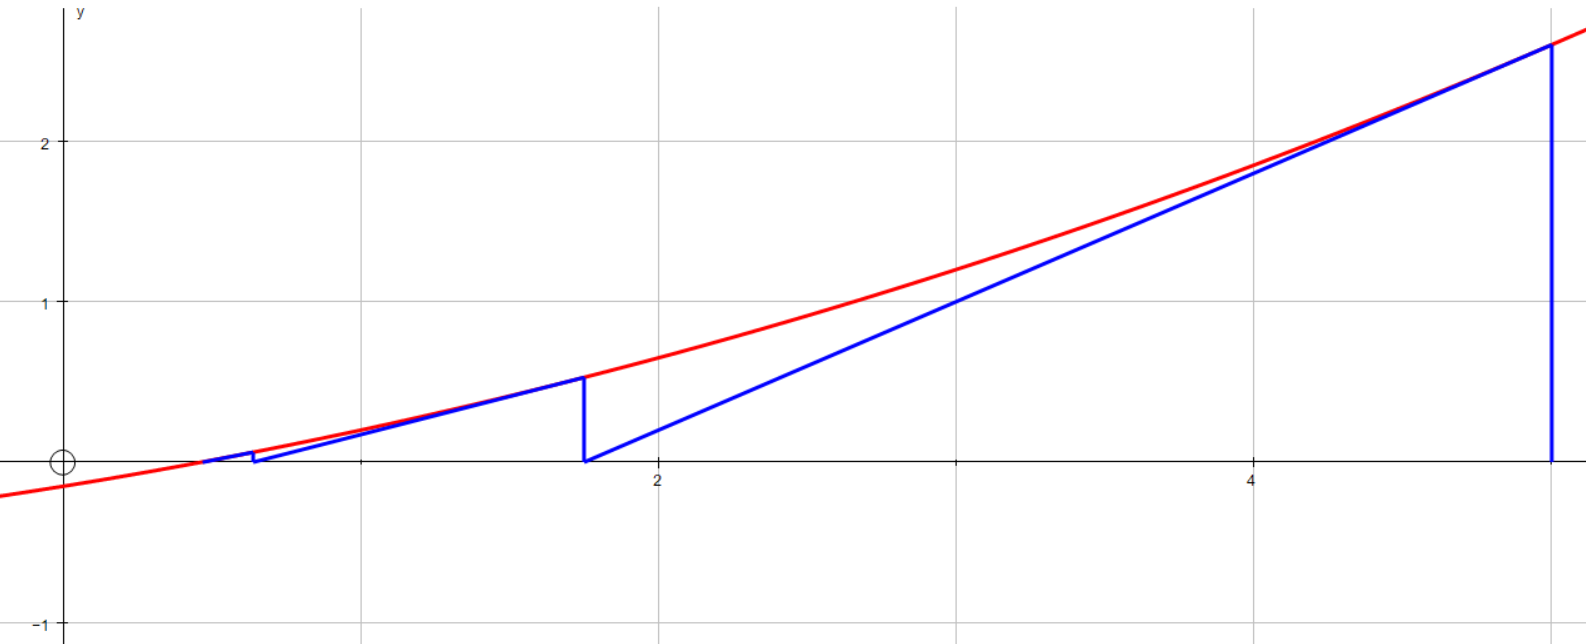
\includegraphics[width=\textwidth]{newtonraphson}}
\end{figure}
A Newton-Raphson iteration is another method for finding a root of an equation. In order to perform one, draw a tangent and follow it towards a root. At its intersection with the $x$-axis, recalculate the tangent with the new $x$-coordinate, and follow the new tangent towards the root. \newline \par

For the curve $y=f(x)$, the tangent at any given point, $\left(x_{n},f\left(x_{n}\right)\right)$ has equation
\begin{equation*}
y-f\left(x_{n}\right)=f'\left(x_{n}\right)\cdot\left(x-x_{n}\right) \\
\end{equation*}
The root of this equation is where $x=x_{n+1}$, and $y=0$. Therefore
\begin{align*}
0-f\left(x_{n}\right)&=f'\left(x_{n}\right)\cdot\left(x_{n+1}-x_{n}\right) \\
& \\
x_{n+1}&=x_{n}-\frac{f\left(x_{n}\right)}{f'\left(x_{n}\right)}
\end{align*}
\vspace{0.5cm}


\subsection{Fixed point iteration}
\begin{itemize}
\item A Level M Year 2 \hspace{1cm} \phantom{ AS / } Pages 313 -- 326
\end{itemize} \par
\begin{figure}[H]
\centering
\scalebox{.5}{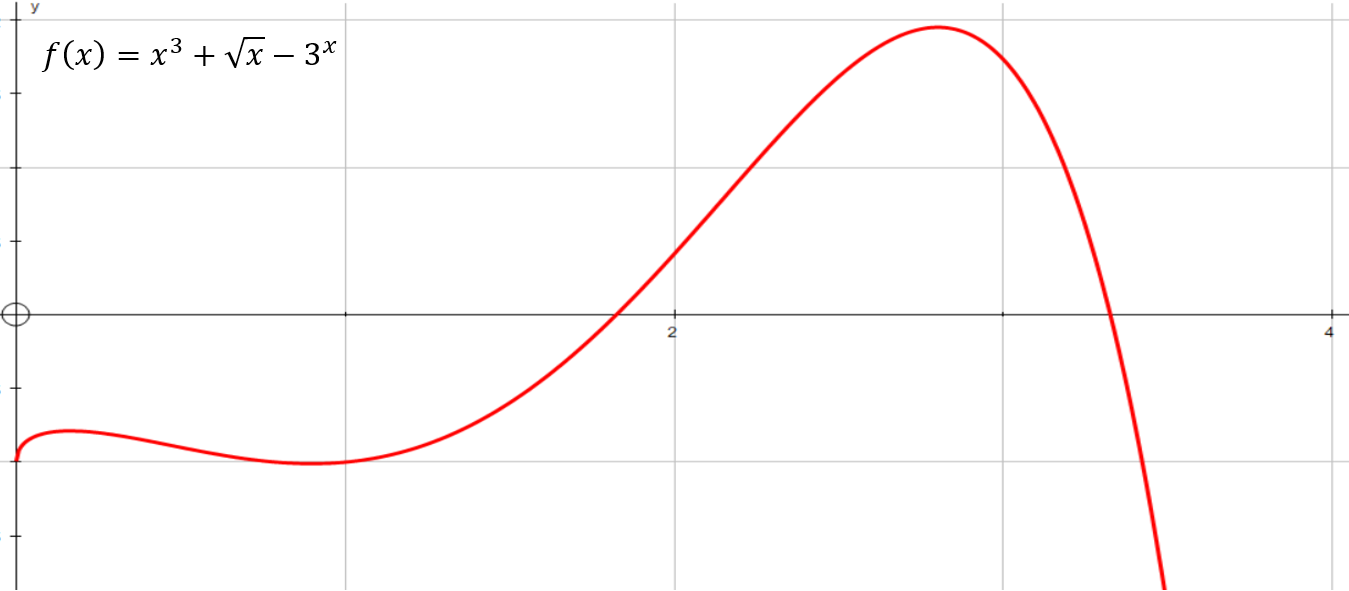
\includegraphics[width=\textwidth]{fixedpointiteration}}
\end{figure}
\begin{itemize}
\item[-] A fixed point of an iterated function is a number that an iteratively defined function converges to from various starting inputs
\item[-] A stable fixed point is one which the function converges to from various inputs. An unstable fixed point returns itself only when it itself is the input.
\end{itemize}
To find an iteration of a function to find a root, rearrange the function to give $x$ in terms of $x$. For example, take the function $x^{5}-3x^{4}+1=0$
\begin{align*}
x&=\sqrt[4]{\frac{x^{5}+1}{3}} & &\text{which converges to }x=0.82328\ldots \\
x&=\sqrt[5]{3x^{4}-1} & &\text{which converges to }x=0.85667\ldots \\
x&=\frac{x^{4}-1}{x^{4}} & &\text{which converges to }x=2.98745\ldots \\
\end{align*}
Another way of thinking about this then is thinking of the roots of $f(x)$ being at the point of the intersection between $y=g(x)$, a function which gives $x$ in terms of $x$, and $y=x$. However the iteration will only converge under the condition that $\left| g'\left( x_{root} \right) \right|<1$ \newline \par

\noindent If:
\begin{flalign*}
0\leq\,&g'\left( x_{root} \right)\leq1 & &\text{The iteration will converge stepwise} \\
1\leq\,&g'\left( x_{root} \right) & &\text{The iteration will diverge stepwise} \\
-1\leq\,&g'\left( x_{root} \right)\leq0 & &\text{The iteration will converge as a spiral} \\
&g'\left( x_{root} \right)\leq-1 & &\text{The iteration will diverge as a spiral}\\
\end{flalign*}
\vspace{0.5cm}


\clearpage
\section{Differential equations}
\vspace{0.5cm}


\subsection{Related rates of change}
\label{relatedratesofchange}
\begin{itemize}
\item A Level M Year 2 \hspace{1cm} \phantom{ AS / } Pages 265 -- 269
\end{itemize} \par
Leibniz notation $\left( \frac{\mathrm{d}}{\mathrm{d}x}\right)$ does not denote a fraction, however it can behave as one. For example, enlarging a square with initital side length of $5\,cm$  and the rate of increase is $3\,cm s^{-1}$, What is the rate of increase in area when the side length is $17\,cm$? \newline \par
\begin{tblr}{lcc}
Variables & $\hspace{.5cm}$Relationships$\hspace{.5cm}$ & Goal \\
$A$, area $\left(cm^{2}\right)$ & $A=x^{2}$ & \\
$x$, side length $\left(cm\right)$ & $\frac{\mathrm{d}x}{\mathrm{d}t}=3$ & $\frac{\mathrm{d}A}{\mathrm{d}t}$\\
$t$, time $\left(s\right)$ &  & \\
\end{tblr}
\begin{align*}
\frac{\mathrm{d}A}{\mathrm{d}x}&=2x & \frac{\mathrm{d}x}{\mathrm{d}t}&=3 & \frac{\mathrm{d}A}{\mathrm{d}x}\times\frac{\mathrm{d}x}{\mathrm{d}t}&=\frac{\mathrm{d}A}{\mathrm{d}t} \\
& & & & 2x\times3&=6x\,cm^{2}\,s^{-1} \\
\end{align*}
\begin{equation*}
\frac{\mathrm{d}A}{\mathrm{d}t}\bigg|_{x=17\,cm}=6\times17=102\,cm^{2}\,s^{-1}
\end{equation*}
\vspace{0.5cm}


\subsection{Separable differential equations}
\begin{itemize}
\item A Level M Year 2 \hspace{1cm} \phantom{ AS / } Pages 283 -- 289
\end{itemize} \par
With some differential equations, it is possible to make $\frac{\mathrm{d}y}{\mathrm{d}x}$ a multiple of $y$, and then integrate from that step. After integrating, but before rearranging, make sure the constant term is put back in at this step, since it may change from simply being a $+c$ term in its final form. For example;
\begin{flalign*}
\frac{1}{y}\frac{\mathrm{d}y}{\mathrm{d}x}&=x & &\Rightarrow & \ln(y)&=\frac{x^{2}}{2}+c & &y=e^{\frac{x^{2}}{2}+c}=e^{\frac{x^{2}}{2}}\times e^{c}=Ae^{x^{2}} && \\
\frac{1}{y}\frac{\mathrm{d}y}{\mathrm{d}x}&=x & &\nRightarrow & \ln(y)&=\frac{x^{2}}{2} & &y\neq e^{\frac{x^{2}}{2}}+c\phantom{aaa} \textbf{\underline{INCORRECT}} && \\
\end{flalign*}

$Ae^{\frac{x^{2}}{2}}\neq e^\frac{x^{2}}{2}+c$, and so in the correct method, the constant comes out as a coefficient of the `$x$-containing term', whereas just adding it on at the end gives a pure constant to the function.
\vspace{0.5cm}


\subsection{First order linear differential equations -- Integrating factor}
\begin{itemize}
\item A Level FM Year 2 \hspace{1cm} \phantom{AS /} Pages 227 -- 231
\end{itemize} \par
If a first order linear equation in one variable is not separable, for example $\frac{\mathrm{d}y}{\mathrm{d}x}=x^{2}-xy$, we can use the integrating factor method. \newline \par

General first order linear differential equation:
\begin{equation*}
\frac{\mathrm{d}y}{\mathrm{d}x}+P(x)y=Q(x)
\end{equation*} \newline \par

Consider the following
\begin{align*}
\frac{\mathrm{d}}{\mathrm{d}x}\left[ I(x)y \right]=I(x)\frac{\mathrm{d}y}{\mathrm{d}x}+I'(x)y&=I(x)\cdot\frac{\mathrm{d}y}{\mathrm{d}x}+\frac{\mathrm{d}\left[ I(x) \right]}{\mathrm{d}x}\cdot y \\
I(x)\cdot\frac{\mathrm{d}y}{\mathrm{d}x}+\left(I(x)P(x)\right)\cdot y&=I(x)Q(x)
\end{align*}
We need
\begin{equation*}
I(x)P(x)=\frac{\mathrm{d}I}{\mathrm{d}x}
\end{equation*} 
Therefore
\begin{equation*}
\int \frac{1}{I}\,\mathrm{d}I=\int P(x)\,\mathrm{d}x
\end{equation*}
And if
\begin{equation*}
\ln(I(x))=\int P(x)\,\mathrm{d}x
\end{equation*}
Then
\begin{equation*}
I(x)=e^{\int P(x)\,\mathrm{d}x}
\end{equation*} \newline \par

So given a first order linear differential equation which is inseparable $\left(\frac{\mathrm{d}y}{\mathrm{d}x}+P(x)y=Q(x)\right)$, we can multiply it by an \emph{integrating factor}, $I(x)$, to turn it into something of the form:
\begin{equation*}
I(x)\frac{\mathrm{d}y}{\mathrm{d}x}+I'(x)y=I(x)Q(x)
\end{equation*}
Since $I(x)$ is chosen such that $I(x)P(x)=I'(x)$, which is the result of applying a product rule derivative of $I(x)y$ with respect to $x$.
\vspace{0.5cm}


\subsection{Homogeneous second order linear differential equations}
\begin{itemize}
\item A Level FM Year 2 \hspace{1cm} \phantom{AS /} Pages 231 -- 235
\end{itemize} \par
A general second order homogeneous linear differential equation can be expressed in the form
\begin{equation*}
a\frac{\mathrm{d}^{2}y}{\mathrm{d}x^{2}}+b\frac{\mathrm{d}y}{\mathrm{d}x}+cy=0
\end{equation*}
To find a solution, try something of the form
\begin{equation*}
y=e^{\lambda x}
\end{equation*}
When substituted into the general equation this gives
\begin{equation*}
a\lambda^{2}e^{\lambda x}+b\lambda e^{\lambda x} + c e^{\lambda x}=0
\end{equation*}
Dividing through by $e^{\lambda x}$, this yields the \emph{auxiliary equation}
\begin{equation*}
a\lambda^{2}+b\lambda+c=0
\end{equation*}
\begin{itemize}
\item[If:] $\lambda$ has two real roots, the general solution is of the form
\begin{equation*}
y=Ae^{\lambda_{1}x}+Be^{\lambda_{2}x}
\end{equation*}
\item[If:] $\lambda$ has one repeated root, the general solution is of the form
\begin{equation*}
y=Ae^{\lambda x}+Bxe^{\lambda x}
\end{equation*}
\item[If:] $\lambda$ has complex conjugate roots, the general solution is of the form
\begin{equation*}
y=e^{\mathfrak{Re}[\lambda]x}\left(A\cos\left(\mathfrak{Im}[\lambda]x\right)+B\sin\left(\mathfrak{Im}[\lambda]x\right)\right)
\end{equation*}
\end{itemize}
\vspace{0.5cm}


\subsection{Non-homogeneous second order linear differential equations}
\begin{itemize}
\item A Level FM Year 2 \hspace{1cm} \phantom{AS /} Pages 235 -- 240
\end{itemize} \par
A general second order homogeneous linear differential equation can be expressed in the form
\begin{equation*}
a\frac{\mathrm{d}^{2}y}{\mathrm{d}x^{2}}+b\frac{\mathrm{d}y}{\mathrm{d}x}+cy=f(x)
\end{equation*}
The general solution to this is of the form $GS=CF(x)+PI(x)$, where: \newline \par
\noindent $CF(x)$ is a \emph{complementary function} which satisfies:
\begin{equation*}
a\frac{\mathrm{d}^{2}y}{\mathrm{d}x^{2}}+b\frac{\mathrm{d}y}{\mathrm{d}x}+cy=0
\end{equation*}
$PI(x)$ is a \emph{particular integral} which satisfies:
\begin{equation*}
a\frac{\mathrm{d}^{2}y}{\mathrm{d}x^{2}}+b\frac{\mathrm{d}y}{\mathrm{d}x}+cy=f(x)
\end{equation*} \newline \par

\scriptsize
\begin{centering}
\begin{tblr}{|[.75pt]| l | l ||[.75pt]}
\hline[1pt]
\textbf{For a right hand side of the form:} & \textbf{Try a particular integral of the form} \\ \hline[.75pt]
Polynomial & \emph{General polynomial} of the same order \\
\emph{e.g.} $ax^{2}+bx+c$ & \emph{e.g.} $px^{2}+qx+r$ \\ \hline
$ae^{bx}$ & $pe^{bx}$ \\ \hline
$A\cos(\omega x)$ \emph{and / or} $B\sin(\omega x)$ & $p\cos(\omega x)+q\sin(\omega x)\,\,\,$ \tiny{\emph{(Must include both terms)}} \\ \hline[.75pt]
\end{tblr}
\end{centering} \newline \par
\normalsize
Where all constants of the particular integral are to be determined by substituting the trial solution in to the original differential equation.
\vspace{0.5cm}


\subsection{Systems of differential equations}
\begin{itemize}
\item A Level FM Year 2 \hspace{1cm} \phantom{AS /} Pages 256 -- 259
\end{itemize} \par
\begin{align*}
\frac{\mathrm{d}x}{\mathrm{d}t}&=f(x,y,t) & \frac{\mathrm{d}y}{\mathrm{d}t}&=g(x,y,t)
\end{align*}
Where $f$ and $g$ are functions involving $x$, $y$, and $t$. \newline \par

In order to solve, we must eliminate one variable of $x$ and $y$. To do this, rearrange one equation to give $y$ in terms of $x$, $t$, and $\dot{x}$. Differentiate this expression for $y$ to give an expression for $\dot{y}$. Substitute these expressions for $y$, and $\dot{y}$ into the other equation to give a non-homogeneous second order linear differential equation in terms of $x$, and derivatives of $x$ with respect to $t$. Solve to obtain an expression for $x$ in terms of $t$, and then substitute in to one of the original differential equations to find $y$ in terms of $t$. For example;
\begin{align*}
\dot{x}&=4x-y+50\sin(t) &
\dot{y}&=6x-3y+50\cos(t)
\end{align*}
Subject to initial conditions
\begin{align*}
x(t=0)&=0 & y(t=0)&=15
\end{align*}
\begin{align*}
y&=4x-\dot{x}+50\sin(t) & &\Rightarrow & \dot{y} =4-\ddot{x}+50\cos(t)
\end{align*}
\begin{equation*}
4-\ddot{x}+50\cos(t)=6x-3\left(4x-\dot{x}+50\sin(t)\right)+50\cos(t) \\
\end{equation*}
\begin{align*}
\ddot{x}-\dot{x}-6x&=150\sin(t) \\
\lambda^{2}-\lambda-6&=0 \\
(\lambda-3)(\lambda+2)&=0
\end{align*}
\begin{align*}
CF:\hspace{.3cm}&x_{\text{\tiny{$CF$}}}=Ae^{-2t}+Be^{3t} \\
PI:\hspace{.3cm}&x_{\text{\tiny{$PI$}}}=M\sin(t)+N\cos(t)
\end{align*}
\small
\begin{equation*}
(-M\sin(t)-N\cos(t))-(M\cos(t)-N\sin(t))-6(M\sin(t)+N\cos(t))=150\sin(t)
\end{equation*}
\normalsize
\begin{align*}
(-M+N-6M)\sin(t)&=150\sin(t) & (-N-M-6N)\cos(t)&=0 \\
-7M+N&=150 & M+7N&=0 \\
& & M&=-7N \\
-7(-7N)+N&=150 & & \\
50N&=150 & & \\
\end{align*}
\begin{equation*}
N=3 \hspace{.3cm} \Rightarrow \hspace{.3cm} M=-21
\end{equation*}
\begin{equation*}
GS:\,\, x=Ae^{-2t}+Be^{3t}-21\sin(t)+3\cos(t)
\end{equation*}
And from the initial conditions, at $t=0$, $A+B+3=0$. \newline \par

Using the newfound general solution,
\begin{equation*}
\dot{x}=-2Ae^{-2t}+3Be^{3t}-3\sin(t)-21\cos(t)
\end{equation*}
And using one of the initial equations,
\begin{align*}
\dot{x}&=4x_{\text{\tiny{$GS$}}}-y+50\sin(t) \\
&=4\left[ Ae^{-2t}+Be^{3t}-21\sin(t)+3\cos(t) \right] -y+50\sin(t) \\
&=4Ae^{-2t}+4Be^{3t}-84\sin(t)+12\cos(t)-y+50\sin(t) \\
&=4Ae^{-2t}+4Be^{3t}-34\sin(t)+12\cos(t)-y
\end{align*}

Using the initial conditions;
\begin{align*}
\dot{x}&=-2A+3B-0-21 & &\text{Using $GS$} \\
\dot{x}&=4A+4B-0+12-15 & &\text{Using original equation} \\
\end{align*}
\vspace{-1.2cm}
\begin{equation*}
-18=6A+B
\end{equation*} \newline
This gives a pair of simultaneous equations for $A$, and $B$:
\begin{align*}
-18&=6A+B \\
0&=A+B+3 \\
& \\
-18&=6A-3-A \\
-15&=5A \\
& \\
\Rightarrow A&=-3 \\
B&=0
\end{align*}

Therefore,
\begin{equation*}
x_{\text{\tiny{$GS$}}}=-3e^{-2t}+3\cos(t)-21\sin(t)
\end{equation*}
And so
\small
\begin{align*}
y&=-12e^{-2t}+12\cos(t)-84\sin(t)-\left(6e^{-2t}-3\sin(t)-21\cos(t)\right)+50\sin(t) \\
&=-18e^{-2t}+33\cos(t)-31\sin(t)
\end{align*}
\normalsize

Therefore the final solutions for $x$, and $y$, are
\begin{align*}
x&=-3e^{-2t}+3\cos(t)-21\sin(t) \\
y&=-18e^{-2t}+33\cos(t)-31\sin(t)
\end{align*}
\vspace{0.5cm}



\clearpage
\appendix
\appendixpage
\sloppy
\section{OCR course textbooks}
The four course textbooks referred to and referenced can be found here
\begin{itemize}
\item A Level Mathematics for OCR A Student Book 1 (AS / Year 1) -- Vesna Kadelburg and Ben Woolley
\item [] Referred to as \emph{A Level M Year 1}
\begin{itemize}
\item[] \url{https://www.cambridge.org/gb/education/subject/mathematics/a-level-mathematics-ocr-a/a-level-mathematics-ocr-student-book-1-as-year-1?isbn=9781316644287&format=PB}
\end{itemize}
\vspace{.3cm}
\item A Level Mathematics for OCR A Student Book 2 (Year 2) -- Vesna Kadelburg and Ben Woolley
\item [] Referred to as \emph{A Level M Year 2}
\begin{itemize}
\item[] \url{https://www.cambridge.org/gb/education/subject/mathematics/a-level-mathematics-ocr-a/a-level-mathematics-ocr-a-student-book-2-year-2?isbn=9781316644300&format=PB}
\end{itemize}
\vspace{.3cm}
\item A Level Further Mathematics for OCR A Pure Core Student Book 1 (AS / Year 1) -- Vesna Kadelburg and Ben Woolley
\item [] Referred to as \emph{A Level FM Year 1}
\begin{itemize}
\item[] \url{https://www.cambridge.org/gb/education/subject/mathematics/a-level-further-mathematics-ocr-a/a-level-further-mathematics-ocr-a-pure-core-student\\-book-1-as-year-1?isbn=9781316644386&format=PB}
\end{itemize}
\vspace{.3cm}
\item A Level Further Mathematics for OCR A Pure Core Student Book 2 (Year 2) -- Vesna Kadelburg and Ben Woolley
\item [] Referred to as \emph{A Level FM Year 2}
\begin{itemize}
\item[] \url{https://www.cambridge.org/gb/education/subject/mathematics/a-level-further-mathematics-ocr-a/a-level-further-mathematics-ocr-a-pure-core-student\\-book-2-year-2?isbn=9781316644393&format=PB}
\end{itemize}
\end{itemize}


\end{document}